\chapter{Implementazioni e tecnologie}
\label{chap:implementazione}

In questo capitolo vengono descritte in dettaglio le scelte tecnologiche e le strategie implementative adottate per la realizzazione del sistema presentato nel Capitolo 2. L’obiettivo principale è offrire una panoramica completa sull’integrazione tra le diverse componenti software e hardware, evidenziando come la combinazione di tecnologie moderne e soluzioni open-source abbia permesso di ottenere un’infrastruttura scalabile, modulare e facilmente manutenibile.

A partire dalla selezione dello stack tecnologico — sia frontend che backend — vengono illustrate le motivazioni alla base delle scelte compiute, le metodologie di containerizzazione e orchestrazione dei servizi, nonché i pattern di persistenza dei dati strutturati e multimediali. Il capitolo approfondisce inoltre i sistemi di parametrizzazione adattiva per l’ottimizzazione delle performance in relazione all’hardware disponibile, le strategie di resilienza, fault tolerance e gestione degli errori implementate per garantire affidabilità operativa anche in contesti distribuiti.

Attraverso una descrizione puntuale dell’implementazione dei singoli layer funzionali — dalla pre-elaborazione del dato grezzo al training degli algoritmi, fino alla visualizzazione interattiva in ambiente web — il lettore potrà apprezzare l’articolazione della soluzione e comprenderne sia gli aspetti di innovazione tecnica, sia i criteri di progettazione orientati alla flessibilità e alla sperimentazione.



\subsection{Stack Tecnologico Implementato}

\subsubsection{Tecnologie Frontend}

Il frontend utilizza \textbf{Vue.js 3} come framework principale per lo sviluppo dell'interfaccia utente, scelto per il bilanciamento tra semplicità e funzionalità. La visualizzazione 3D è implementata attraverso \textbf{GaussianSplats3D}\footnote{\url{https://github.com/mkkellogg/GaussianSplats3D}}, una libreria specializzata basata su \textbf{Three.js} che non supporta, nativamente, il rendering di primitive gaussiane.

\subsubsection{Tecnologie di backend}

Il backend è implementato in \textbf{Python} con \textbf{FastAPI} come framework per le API REST, scelto per le performance superiori e la generazione automatica di documentazione OpenAPI. La gestione asincrona utilizza le capacità native di Python con \textbf{asyncio}.

\subsubsection{Infrastruttura e Persistenza}

L'infrastruttura utilizza \textbf{Docker e Docker Compose} per la containerizzazione e l'orchestrazione locale, \textbf{RabbitMQ} come message broker per la comunicazione asincrona, \textbf{MongoDB} come database NoSQL per metadati, e \textbf{Amazon S3} per lo storage oggetti scalabile.

\subsubsection{Pre-elaborazione specializzata}

I servizi di processing integrano \textbf{COLMAP}\footnote{\url{https://https://colmap.github.io}} per Structure from Motion e per i training services, e \textbf{Sharp Frames}\footnote{\url{https://github.com/Reflct/sharp-frames-python}} per l'estrazione video. Ogni servizio è ottimizzato per l'utilizzo specifico di risorse GPU attraverso configurazioni CUDA dedicate.

L'architettura complessiva garantisce scalabilità, manutenibilità e performance ottimali per l'elaborazione di contenuti 3D, fornendo una base solida per l'implementazione dei componenti specializzati descritti nei capitoli successivi.

\subsubsection{Algoritmi di Training integrati}
Il sistema integra progetti open-source specializzati per il training di rappresentazioni 3D:
\begin{itemize}
	\item \textbf{3D Gaussian Splatting
		for Real-Time Radiance Field Rendering}\footnote{\url{https://github.com/graphdeco-inria/gaussian-splatting}} per la generazione di primitive gaussiane da dataset fotografici
	\item \textbf{3D Gaussian Splatting as Markov Chain Monte Carlo
	}\footnote{\url{https://github.com/ubc-vision/3dgs-mcmc}} con l'introduzione di rumore stocastico nel calcolo dei gradienti
	\item \textbf{Taming 3DGS: High-Quality Radiance Fields with Limited Resources
	}\footnote{\url{https://github.com/ubc-vision/3dgs-mcmc}} per la generazione efficiente di scene 3D con vincoli computazionali ridotti
\end{itemize}
Questi progetti sono stati integrati come servizi containerizzati nel workflow di elaborazione, mantenendo la compatibilità con le implementazioni originali e permettendo aggiornamenti indipendenti.

\subsection{Servizi containerizzati}
\label{sec:servizi_containerizzati}

Per garantire modularità, scalabilità e portabilità del sistema, ciascun componente è stato containerizzato tramite \textbf{Docker}. L'intera infrastruttura si basa su microservizi che comunicano tra loro attraverso una rete virtuale comune, orchestrati da \textbf{Docker Compose}.

Ogni container svolge un ruolo specifico e indipendente nel flusso di elaborazione, riducendo le dipendenze tra i moduli. Di seguito si elencano i principali container e le loro funzioni:

\begin{itemize}
	\item \textbf{Accesso e orchestrazione}
	\begin{itemize}
		\item \textbf{api-gateway}: gestisce il routing delle richieste HTTP verso i microservizi interni.
		\item \textbf{job-executor}: coordina i task tra i moduli e comprende alcune parti di pre e post processing.
	\end{itemize}
	
	\item \textbf{Motori di training e rendering 3D}
	\begin{itemize}
		\item \textbf{gaussian-splatting-api}: esegue il training del Gaussian Splatting 3D e si basa sul paper originale.
		\item \textbf{3dgs-mcmc-api}: esegue il training del Gaussian Splatting 3D con la variante Monte Carlo as Markov Chain.
		\item \textbf{taming-3dgs-api}: motore alternativo di training per scene 3D controllate.
	\end{itemize}
	
	\item \textbf{Pre-elaborazione}
	\begin{itemize}
		\item \textbf{colmap-converter}: wrapper per Colmap, utilizzato per la ricostruzione di point cloud a partire da immagini RGB.
	\end{itemize}
	
	\item \textbf{Persistenza e messaggistica}
	\begin{itemize}
		\item \textbf{mongo}: database NoSQL per la persistenza dei dati.
		\item \textbf{rabbitmq}: message broker per la comunicazione asincrona tra i servizi.
	\end{itemize}
	
	\item \textbf{Visualizzazione}
	\begin{itemize}
		\item \textbf{web-viewer}: interfaccia frontend per l'interazione con il workflow di training e la visualizzazione dei risultati 3D generati.
	\end{itemize}
\end{itemize}

\subsubsection{Esempio di Dockerfile: Gaussian Splatting}
Di seguito è riportato un esempio di \texttt{Dockerfile} utilizzato per il container \texttt{gaussian-splatting}, responsabile del rendering 3D basato su rappresentazioni gaussiane. L'immagine si basa su un container NVIDIA compatibile con CUDA e contiene tutte le dipendenze necessarie per eseguire il motore grafico:

\begin{lstlisting}[language=docker, caption={Dockerfile per gaussian-splatting}, label={lst:dockerfile_gs}]
	FROM nvidia/cuda:12.2.2-cudnn8-devel-ubuntu22.04
	ENV DEBIAN_FRONTEND=noninteractive
	
	# Installazione dipendenze di sistema
	RUN apt update && apt upgrade -y && apt install -y \
	git cmake libxmu-dev libxi-dev libgl-dev libomp-dev \
	python3-dev python3-venv python3-pip build-essential ninja-build wget \
	libboost-program-options-dev libboost-filesystem-dev libboost-graph-dev \
	libboost-system-dev libboost-test-dev libeigen3-dev libflann-dev \
	libfreeimage-dev libmetis-dev libgoogle-glog-dev libgflags-dev \
	libsqlite3-dev libglew-dev qtbase5-dev libqt5opengl5-dev libcgal-dev \
	gcc-10 g++-10 libatlas-base-dev libsuitesparse-dev
	
	# Clonazione del repository
	WORKDIR /workspace
	RUN git clone https://github.com/graphdeco-inria/gaussian-splatting --recursive
	
	# Installazione dipendenze Python
	COPY requirements.txt /workspace/gaussian-splatting/
	WORKDIR /workspace/gaussian-splatting
	RUN pip3 install --upgrade pip && \
	pip3 install torch torchvision --extra-index-url https://download.pytorch.org/whl/cu121 && \
	pip3 install -r requirements.txt
	
	# Compilazione moduli C++
	RUN cd submodules/diff-gaussian-rasterization && pip3 install .
	RUN cd submodules/simple-knn && pip3 install .
	RUN cd submodules/fused-ssim && pip3 install .
	
	# Supporto Depth Anything V2
	WORKDIR /workspace
	RUN git clone https://github.com/DepthAnything/Depth-Anything-V2.git
	WORKDIR /workspace/Depth-Anything-V2
	RUN pip3 install opencv-python transformers pillow numpy matplotlib
	RUN mkdir -p checkpoints && \
	wget -O checkpoints/depth_anything_v2_vitl.pth \
	https://huggingface.co/depth-anything/Depth-Anything-V2-Large/resolve/main/depth_anything_v2_vitl.pth
	
	# Ritorno alla directory principale
	WORKDIR /workspace/gaussian-splatting
	CMD ["bash"]
\end{lstlisting}

In seguito, viene definita un'estensione del container per esporre un'interfaccia \texttt{FastAPI}, utile per l'interazione RESTful con il modulo computazionale:

\begin{lstlisting}[language=docker, caption={Estensione API FastAPI per Gaussian Splatting}, label={lst:dockerfile_api}]
	FROM gaussian-splatting
	
	ARG API_PORT=8100
	ENV API_PORT=$API_PORT
	EXPOSE $API_PORT
	
	WORKDIR /workspace/gaussian-splatting
	COPY api.py /workspace/gaussian-splatting/api.py
	
	RUN mkdir -p /tmp/runtime-root && chmod 0700 /tmp/runtime-root
	ENV QT_QPA_PLATFORM=offscreen
	ENV PYTHONUNBUFFERED=1
	
	RUN pip3 install fastapi uvicorn
	
	CMD ["/bin/bash", "-c", "uvicorn api:app --host 0.0.0.0 --port $API_PORT"]
\end{lstlisting}

Questa struttura modulare consente di disaccoppiare il motore grafico dall’interfaccia espositiva, migliorando la manutenibilità e favorendo l’integrazione in pipeline distribuite.
\newpage
\section{Sistema di parametrizzazione adattiva per livelli di qualità e auto-scaling hardware}

Il workflow implementa un sistema di parametrizzazione multi-livello progettato per bilanciare qualità dell'output e vincoli hardware, provando a garantire sempre la generazione di un modello 3D indipendentemente dalle limitazioni del sistema. Tale parametrizzazione cerca di far coesistere i seguenti aspetti:

\begin{itemize}
	\item \textbf{Livelli di qualità utente}: l'utente può scegliere tra tre preset (Fast, Balanced, Quality) che influenzano parametri critici come risoluzione target, numero di frame estratti, iterazioni di training e soglie di densificazione. Questa scelta rappresenta l'\textbf{intento} di qualità desiderato, ma non è vincolante per l'esecuzione.
	
	\item \textbf{Hardware adaptation e graceful degradation}: il sistema, tramite il TrainingParamsService, rileva la VRAM disponibile e applica un downscaling conservativo dei parametri critici (risoluzione, batch size, frame count, ecc.). Questo approccio di graceful degradation è implementato solo in fase di setup: il sistema preferisce ridurre preventivamente la qualità dell’output per prevenire errori di esaurimento risorse (OOM) o crash del container. Una volta avviato il workflow, non sono previsti adattamenti dinamici.

\end{itemize}

\subsection{Struttura dei parametri}

La configurazione di ogni algoritmo è organizzata in categorie distinte, ciascuna con uno scopo specifico nel workflow:

\begin{itemize}
\item \textbf{\texttt{base\_params}}: definiscono i valori di partenza dell'algoritmo, tipicamente corrispondenti ai parametri di default della implementazione originale. Rappresentano la base dalla quale vengono costruiti tutti e tre i livelli di qualità attraverso l'applicazione dei moltiplicatori. Questi parametri influenzano direttamente il comportamento degli algoritmi di training (numero di iterazioni, soglie di densificazione, intervalli di ottimizzazione).

\item \textbf{\texttt{quality\_multipliers}}: moltiplicatori che vengono applicati esclusivamente ai \texttt{base\allowbreak\_params} per generare i parametri finali di training per ciascun livello di qualità. Il livello "fast" riduce tipicamente le iterazioni e accelera il processo, mentre "quality" incrementa la precisione computazionale a scapito dei tempi di elaborazione.

\item \textbf{\texttt{preprocessing\_params}}: parametri che influenzano esclusivamente la fase di preprocessing (estrazione frame, ridimensionamento video) e che non vengono passati agli algoritmi di training. Include risoluzione target e numero di frame da estrarre, parametri che impattano sulla qualità del dataset di input ma rimangono esterni alla logica di training.

\item \textbf{\texttt{manual\_overrides}}: parametri opzionali che possono essere specificati manualmente dall’utente (o dal chiamante API) per forzare valori di training specifici. Gli override hanno priorità su qualsiasi altro parametro calcolato o derivato dai preset, adattamenti hardware e moltiplicatori di qualità. 

\item \textbf{\texttt{hardware\_config}}: definisce le soglie VRAM e le formule di scaling automatico. I \texttt{resolution\_thresholds} stabiliscono le risoluzioni massime supportate per ogni configurazione hardware, le \texttt{scaling\_formulas} permettono un adattamento dinamico dei parametri di training in base alla memoria disponibile.
\end{itemize}


\subsection{Processo di Calcolo Parametri}

Il \texttt{TrainingParamsService} implementa una pipeline di calcolo che trasforma le configurazioni di base in parametri finali pronti per l'esecuzione:

\begin{figure}[htbp]
	\centering
	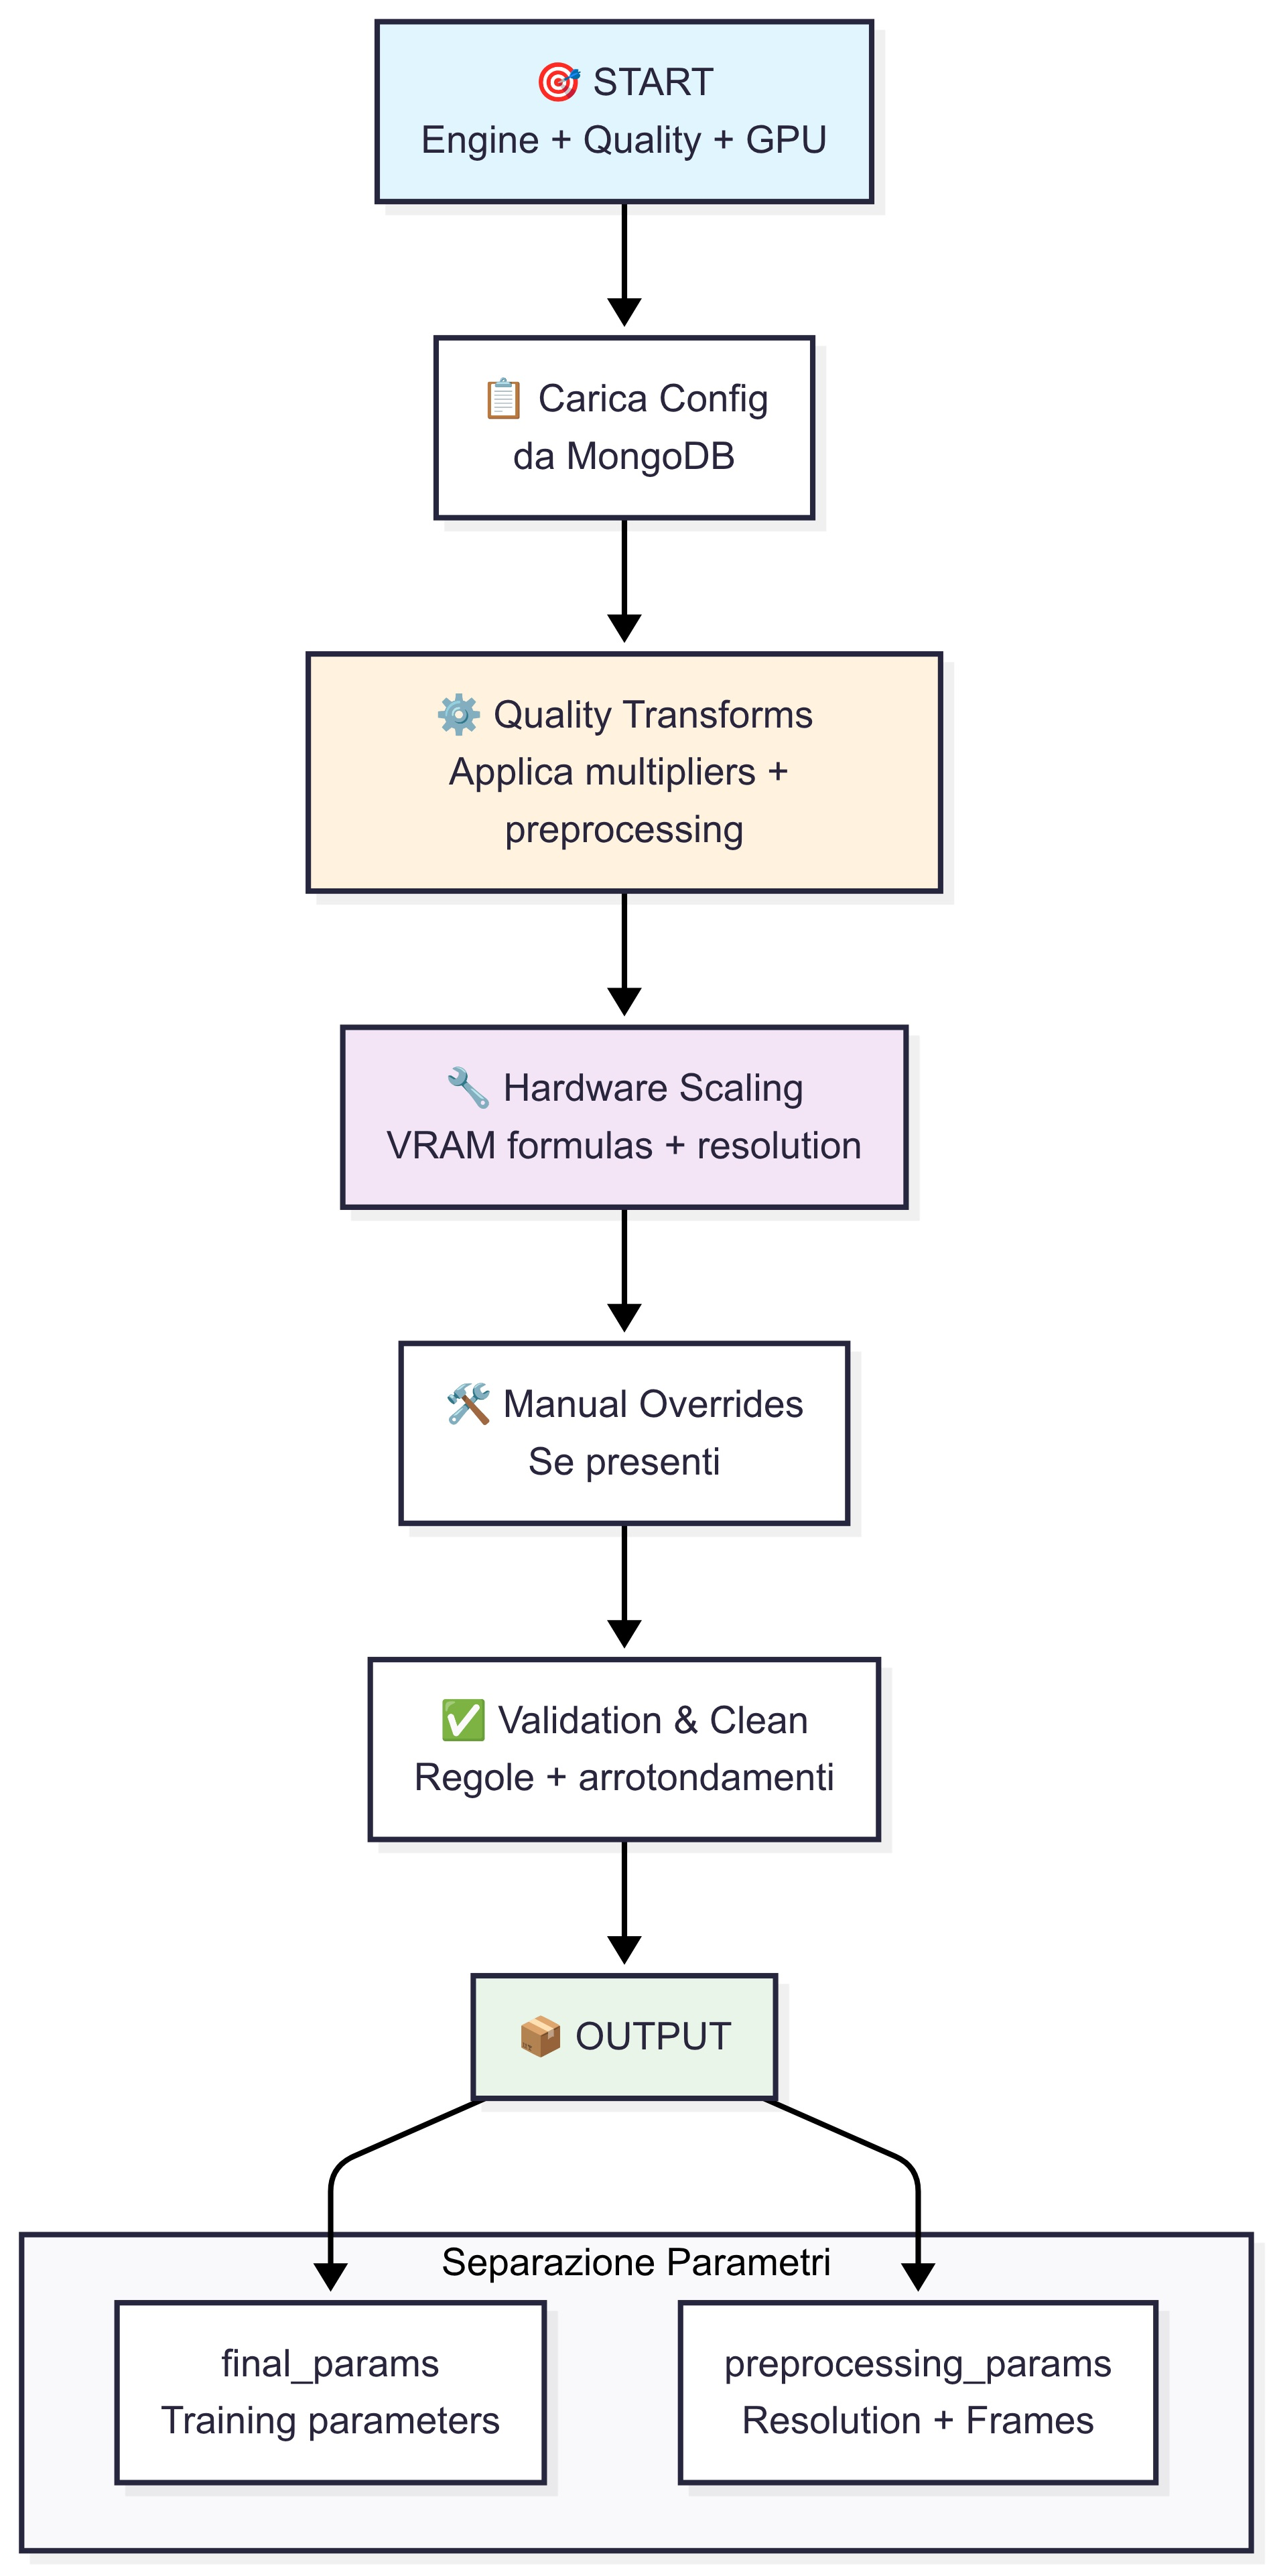
\includegraphics[width=0.7\textwidth]{images/training_params_service_workflow.jpg}
	\caption{Workflow della generazione dei parametri adattivi}
	\label{fig:training_params_service_workflow}
\end{figure}

La separazione netta tra parametri di training e preprocessing consente al sistema di adattare indipendentemente la qualità del dataset di input (risoluzione, numero di frame) e la precisione computazionale del training, ottimizzando l'utilizzo delle risorse hardware disponibili.

\subsection{Configurabilità e Sperimentazione}

Un aspetto fondamentale dell'architettura è la \textbf{persistenza delle configurazioni in MongoDB}, che offre all'owner dell'applicazione la possibilità di modificare dinamicamente i parametri senza dover ricompilare o ridistribuire il software. Questa caratteristica è particolarmente vantaggiosa per:

\begin{itemize}
	\item \textbf{Ottimizzazione empirica}: L'owner può testare diverse combinazioni di parametri, moltiplicatori di qualità e soglie hardware per trovare il bilanciamento ottimale tra qualità dell'output e performance del sistema. Le modifiche alle configurazioni diventano immediatamente operative per tutti i nuovi job.
	
	\item \textbf{Adattamento hardware-specifico}: Ogni deployment può essere fine-tuned per l'hardware specifico disponibile, le \texttt{resolution\_thresholds} e le \texttt{scaling\_formulas} vengono modificate in base alle caratteristiche delle GPU installate e ai risultati dei test empirici.
	
	\item \textbf{Evoluzione degli algoritmi}: L'aggiunta di nuovi algoritmi o l'aggiornamento di quelli esistenti richiede solamente l'inserimento di un nuovo documento nella collection \texttt{training\_params}, mantenendo la retrocompatibilità con il codice esistente.
\end{itemize}

Questa flessibilità consente un approccio iterativo al miglioramento delle performance, dove l'esperienza operativa può guidare l'evoluzione delle configurazioni verso setup sempre più ottimizzati per il contesto di deployment specifico.

\section{Layer di Storage}

Il layer di storage è implementato seguendo una strategia di persistenza ibrida che combina MongoDB per i metadati strutturati e Amazon S3 per lo storage di contenuti multimediali e modelli 3D. Questa architettura ottimizza l'accesso ai dati in base ai pattern di utilizzo specifici di ogni tipo di informazione.

\subsection{MongoDB - Database dei metadati}

MongoDB è configurato come replica set per garantire consistenza e supportare operazioni di change stream necessarie per le notifiche real-time.
Il database è organizzato in tre collection principali, ciascuna ottimizzata per specifici pattern di accesso:

\subsubsection{Collection "models"}
La collection principale memorizza i metadati dei modelli 3D e il tracking delle fasi di elaborazione:

\begin{lstlisting}[language=javascript, caption=Struttura documento modello]
	{
		"_id": "ObjectId",
		"model_name": "Video Demo 1",
		"created_at": "2024-07-24T10:30:00Z",
		"video_s3_key": "videos/uuid-123/input_video.mp4",
		"zip_model_suffix": "3d_model.zip",
		"overall_status": "COMPLETED",
		"current_phase": "metrics_evaluation",
		"parent_model_id": null,  // Per supportare la fork
		
		// Tracking dettagliato delle fasi
		"phases": {
			"frame_extraction": {
				"status": "COMPLETED",
				"started_at": "2024-07-24T10:30:00Z",
				"completed_at": "2024-07-24T10:32:00Z",
				"metadata": {
					"frame_count": 180,
					"processing_params": {"fps": 6, "width": 1920}
				}
			},
			"training": {
				"status": "COMPLETED",
				"metadata": {
					"training_duration_seconds": 1847.3,
					"training_parameters": {
						"engine": "INRIA",
						"quality_level": "balanced",
						"final_params": {"iterations": 30000, "lr": 0.0025}
					}
				}
			},
			"metrics_evaluation": {
				"status": "COMPLETED",
				"metadata": {
					"metrics": {
						"PSNR": 28.45,
						"SSIM": 0.89,
						"LPIPS": 0.12
					}
				}
			}
		},
		
		// Configurazione training
		"training_config": {
			"engine": "INRIA",
			"quality_level": "balanced"
		}
	}
\end{lstlisting}

\textbf{Motivazioni del design}:
\begin{itemize}
	\item \textbf{Struttura denormalizzata}: Le fasi sono embedded nel documento per ridurre le query multiple
	\item \textbf{Metadati flessibili}: Schema dinamico per adattarsi ai diversi tipi di informazioni per fase
	\item \textbf{Supporto fork}: Il campo \texttt{parent\_model\_id} abilita la creazione di varianti (fork)
	\item \textbf{Tracking temporale}: Timestamp dettagliati per analisi performance e debugging
\end{itemize}

\subsubsection{Collection \texttt{"training\_params"}}
Memorizza le configurazioni degli algoritmi con parametrizzazione multi-livello:

\begin{lstlisting}[language=javascript, caption=Struttura configurazione algoritmo]
	{
		"algorithm_name": "gaussian_splatting_original",
		"display_name": "3D Gaussian Splatting (Fixed Iterations)",
		"version": "1.5",
		"active": true,
		
		// Parametri base (livello balanced)
		"base_params": {
			"iterations": 30000,
			"densify_grad_threshold": 0.0002,
			"densification_interval": 100,
			"eval": true
		},
		
		// Moltiplicatori per livelli di qualità
		"quality_multipliers": {
			"fast": {"iterations": 0.8, "densify_grad_threshold": 1.2},
			"balanced": {"iterations": 1.0, "densify_grad_threshold": 1.0},
			"quality": {"iterations": 1.2, "densify_grad_threshold": 0.8}
		},
		
		// Configurazione hardware-specific
		"hardware_config": {
			"baseline_vram_gb": 24,
			"min_vram_gb": 8,
			"resolution_thresholds": [
			{"vram_threshold": 24, "target_width": 3840, "target_height": 2160},
			{"vram_threshold": 16, "target_width": 1920, "target_height": 1080}
			],
			"scaling_formulas": {
				"densify_grad_threshold": {
					"formula": "max(1.0, 2.5 - (vram_factor * 1.5))",
					"min": 1.0, "max": 4.0
				}
			}
		}
	}
\end{lstlisting}
\newpage
\textbf{Vantaggi dell'approccio}:
\begin{itemize}
	\item \textbf{Configurabilità runtime}: Modifiche ai parametri senza redeploy
	\item \textbf{Sperimentazione facilitata}: Test di configurazioni diverse per ottimizzazioni
	\item \textbf{Adattamento hardware}: Scaling automatico basato su VRAM disponibile
	\item \textbf{Versionamento}: Tracking delle evoluzioni delle configurazioni
\end{itemize}

\subsubsection{Collection \texttt{"users"}}
Sistema di autenticazione con ruoli e gestione sessioni:

\begin{lstlisting}[language=javascript, caption=Struttura utente]
	{
		"_id": "ObjectId",
		"username": "admin",
		"hashed_password": "$2b$12$...",  // bcrypt hash
		"role": "admin",
		"created_at": "2024-07-24T10:00:00Z",
		"last_login": "2024-07-24T15:30:00Z"
	}
\end{lstlisting}

\subsection{Amazon S3 - Object Storage}

\subsubsection{Organizzazione Bucket e Prefissi}

Il sistema utilizza una strategia di organizzazione gerarchica su S3 per ottimizzare l'accesso e la gestione del ciclo di vita dei contenuti:
\newline
\dirtree{%
	.1 s3://3dgs-bucket/.
	.2 videos/.
	.3 \{model\_id\}/.
	.4 input\_video.mp4.
	.2 delivery/.
	.3 \{model\_id\}/.
	.4 3d\_model.zip.
	.2 staging/.
	.3 \{model\_id\}/.
	.4 phase\_frame\_extraction.zip.
	.4 point\_cloud\_building\_phase.zip.
	.4 training\_phase.zip.
}

\subsubsection{Gestione contenuti per tipologia}

\paragraph{Video sorgente (videos/)}
I video originali caricati dagli utenti vengono memorizzati con chiavi UUID per evitare conflitti e garantire privacy:

\begin{lstlisting}[language=python, caption=Generazione chiave video]
	upload_id = str(uuid4())
	s3_key = f"videos/{upload_id}/input_video.mp4"
	presigned_url = repository_service.generate_presigned_url_upload(s3_key, content_type)
\end{lstlisting}

\textbf{Caratteristiche}:
\begin{itemize}
	\item \textbf{Upload diretto}: Utilizzo di presigned URL per evitare transito attraverso backend
	\item \textbf{Retention policy}: Possibile archiviazione automatica dopo completamento processing
	\item \textbf{Versioning}: Supporto per multiple versioni dello stesso contenuto
\end{itemize}

\paragraph{Modelli finali (delivery/)}
I modelli 3D ottimizzati per la visualizzazione web vengono memorizzati in formato compresso ed ogni archivio contiene la cloud point finale in formato .ksplat e la lista delle camere in formato .json prodotte dall'algoritmo di training:

\begin{lstlisting}[language=python, caption=Upload modello finale]
	zip_model_s3_key = f"delivery/{model_id}/3d_model.zip"
	# Contiene: point_cloud.ksplat + cameras.json
	repository_service.upload(zip_filename, zip_model_s3_key)
\end{lstlisting}

\textbf{Ottimizzazioni}:
\begin{itemize}
	\item \textbf{Formato KSPLAT}: Conversione da PLY per ridurre dimensioni e ottimizzare rendering
	\item \textbf{CDN integration}: Possibile distribuzione attraverso CloudFront per performance globali
	\item \textbf{Caching headers}: Configurazione per ottimizzare caching browser
\end{itemize}

\paragraph{Dati Intermedi (staging/)}
Le fasi intermedie vengono persistite per supportare fork, retry e debugging:

\begin{lstlisting}[language=python, caption=Pattern salvataggio fase intermedia]
	phase_zip_s3_key = f"staging/{parent_model_id}/{PHASE_NAME}_phase.zip"
	phase_zip_helper.create_phase_zip_and_upload(model_id, model_dir, PHASE_NAME, directories)
\end{lstlisting}

\textbf{Benefici}:
\begin{itemize}
	\item \textbf{Recuperabilità}: Possibilità di ripartire da fasi intermedie in caso di errori
	\item \textbf{Sperimentazione}: Fork di modelli per testare algoritmi diversi senza reprocessing completo
	\item \textbf{Debugging}: Accesso ai dati intermedi per analisi e ottimizzazioni
\end{itemize}

\subsubsection{Pattern di Accesso Ottimizzati}

\paragraph{Workflow di elaborazione}
Durante l'elaborazione, il sistema implementa un pattern cache-first per ottimizzare l'I/O:

\begin{lstlisting}[language=python, caption=Pattern cache-first per dati S3]
	# 1. Verifica cache locale
	if os.path.exists(local_cache_path) and is_valid_cache(local_cache_path):
	return local_cache_path
	
	# 2. Download da S3 con caching
	repository_service.download(s3_key, local_path)
	update_cache_metadata(local_path)
	return local_path
\end{lstlisting}
\newpage
\paragraph{Frontend Access Pattern}
Per l'accesso frontend, il sistema combina metadata queries su MongoDB con contenuti diretti da S3:

\begin{lstlisting}[language=python, caption=Pattern accesso ibrido frontend]
	# 1. Recupera metadati da MongoDB
	model_metadata = model_service.get_model_by_id(model_id)
	
	# 2. Genera URL diretto per contenuti S3
	if model_metadata.zip_model_suffix:
	model_url = f"https://s3.amazonaws.com/bucket/delivery/{model_id}/{model_metadata.zip_model_suffix}"
	
	return {
		"metadata": model_metadata,
		"model_download_url": model_url
	}
\end{lstlisting}

Questa strategia ibrida garantisce performance ottimali combinando la flessibilità di MongoDB per query complesse sui metadati con la scalabilità e durabilità di S3 per contenuti di grandi dimensioni.

\section{Layer di Orchestrazione}
Il layer di orchestrazione coordina in modo asincrono l'esecuzione sequenziale delle cinque fasi di elaborazione del workflow. L'implementazione si basa su RabbitMQ come message broker e implementa un pattern Producer-Consumer specializzato per gestire workflow di training complessi con supporto per operazioni di retry e fork.

\subsection{Code di messaggi e configurazione RabbitMQ}

Il sistema implementa cinque code dedicate, ciascuna responsabile di una fase specifica del workflow:

\begin{lstlisting}[language=python, caption=Definizione code specializzate per workflow]
	queues = [
	'frame_extraction_queue',      # Fase 1: Estrazione frame video
	'point_cloud_queue',           # Fase 2: Generazione nuvola punti  
	'model_training_queue',        # Fase 3: Training algoritmi GS
	'upload_queue',                # Fase 4: Upload modello 3D
	'metrics_generation_queue'     # Fase 5: Calcolo metriche qualità
	]
\end{lstlisting}

\subsubsection{Configurazione di persistenza e acknowledgment}

Ogni coda è configurata per garantire la massima affidabilità del sistema:

\begin{itemize}
	\item \textbf{Persistenza delle code}: \texttt{durable=True} garantisce che le code sopravvivano ai riavvii del broker
	\item \textbf{Persistenza dei messaggi}: \texttt{delivery\_mode=2} assicura che tutti i messaggi siano scritti su disco
	\item \textbf{Acknowledgment immediato}: I messaggi RabbitMQ vengono consumati e confermati immediatamente dopo la lettura e il parsing, prima dell'avvio del job vero e proprio. Questo garantisce che i messaggi non rimangano bloccati in coda in caso di problemi durante l'elaborazione e permette di interrompere definitivamente job problematici tramite il restart dei container, senza che questi vengano automaticamente riprocessati.
\end{itemize}

\subsubsection{Monitoraggio RabbitMQ}

Il sistema fornisce visibilità completa attraverso la RabbitMQ Management Interface, che offre monitoraggio real-time delle code, includendo:

\begin{itemize}
	\item Numero di messaggi in attesa per ogni coda
	\item Throughput e metriche di performance
	\item Stato delle connessioni producer-consumer
	\item Gestione delle connessioni dedicate e isolate tra API Gateway (producer) e Job Executor (consumer)
\end{itemize}

\begin{figure}[h]
	\centering
	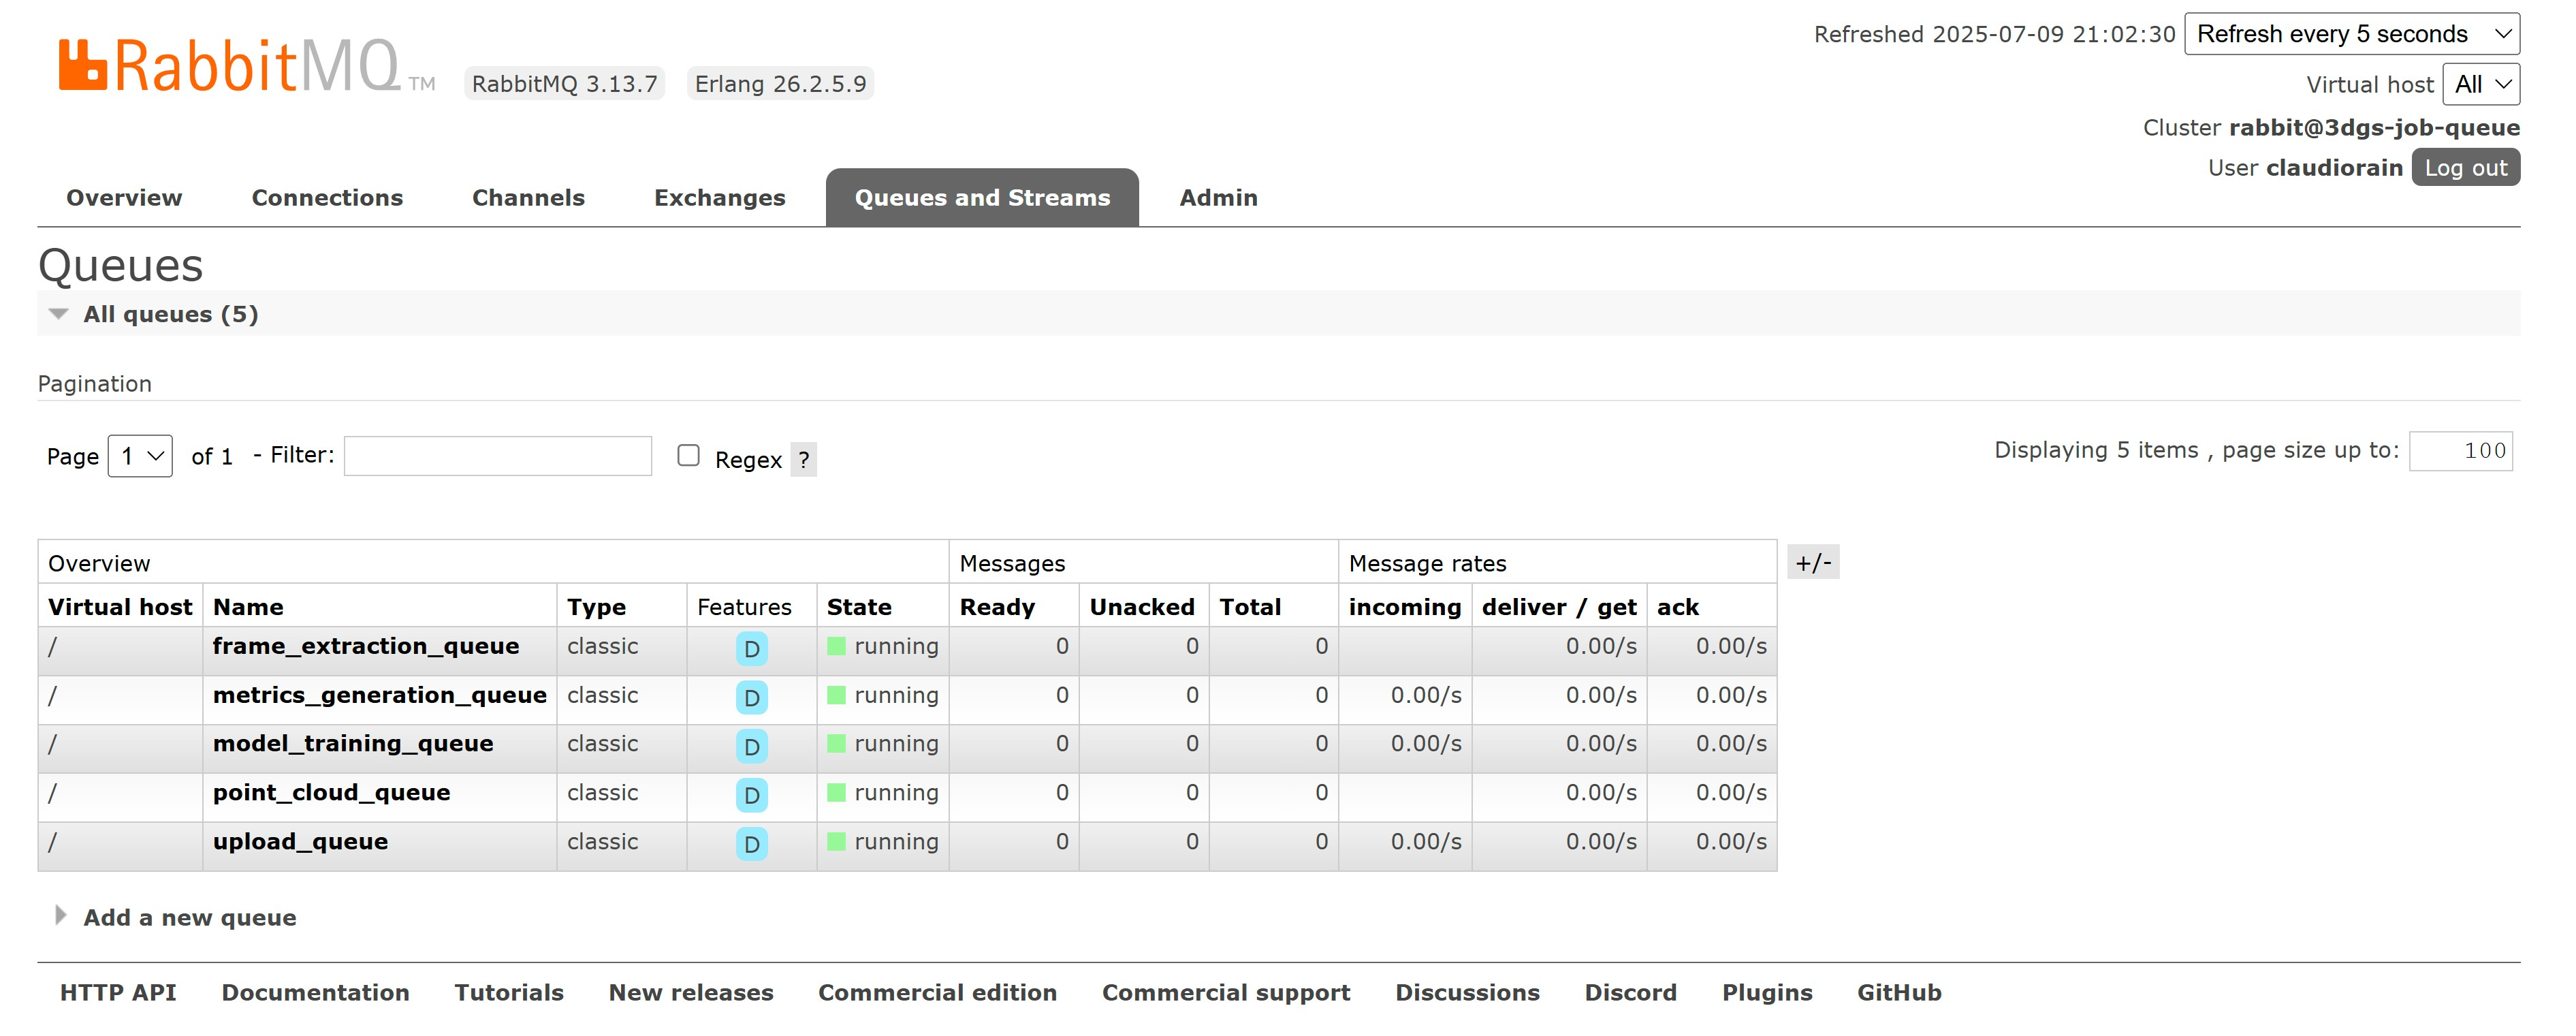
\includegraphics[width=\textwidth]{images/rabbitmq_queues_interface.jpg}
	\caption{Interfaccia di gestione RabbitMQ - Vista code attive del sistema}
	\label{fig:rabbitmq_queues}
\end{figure}

\subsection{Pattern Producer-Consumer ibrido}

Il sistema implementa una variante specializzata del pattern Producer-Consumer tradizionale, dove il Job Executor assume alternativamente i ruoli di consumer e producer durante l'esecuzione del workflow sequenziale. Questa architettura elimina la necessità di un coordinatore esterno e garantisce un flusso continuo attraverso le cinque fasi di elaborazione.

\subsubsection{Architettura del Pattern}

Il pattern si basa su due componenti principali con responsabilità distinte:

\begin{itemize}
	\item \textbf{API Gateway - Producer Esclusivo}: funge da punto di ingresso del sistema, responsabile esclusivamente dell'inserimento dei job iniziali nelle code appropriate. Utilizza un mapping standardizzato fase-coda per determinare il punto di partenza del workflow (fork e retry).
	
	\item \textbf{Job Executor - Consumer-Producer ibrido}: implementa il cuore del pattern attraverso un comportamento duale che si alterna dinamicamente durante l'elaborazione. Opera come consumer durante l'estrazione e il processing dei messaggi dalle code, quindi assume il ruolo di producer per l'invio del job alla fase successiva.
\end{itemize}

\subsubsection{Meccanismo di Funzionamento}

Il workflow segue un ciclo continuo strutturato in tre fasi principali:

\begin{enumerate}
	\item \textbf{Fase Consumer}: Il Job Executor controlla sequenzialmente le code tramite polling attivo, utilizzando il metodo \texttt{process\_queues\_sequentially} che implementa un ciclo di controllo continuo su tutte le code del sistema.
	
	\item \textbf{Fase Processing}: Una volta estratto un messaggio, il sistema utilizza un dispatcher centralizzato che effettua il routing verso l'handler specifico in base alla coda di origine (\texttt{handle\_frame\_extraction}, \texttt{handle\_point\_cloud\_building}, etc.).
	
	\item \textbf{Fase Producer}: Al completamento dell'elaborazione, \texttt{send\_to\_next\_phase} implementa la transizione dal ruolo consumer al ruolo producer, inserendo automaticamente il job nella coda della fase successiva.
\end{enumerate}
\newpage
\subsubsection{Vantaggi Architetturali}

Questo approccio offre diversi benefici rispetto a implementazioni tradizionali:

\begin{itemize}
	\item \textbf{Coordinamento automatico}: Ogni fase completata innesca automaticamente la successiva, eliminando la necessità di coordinamento esterno
	\item \textbf{Resilienza}: I messaggi persistenti garantiscono la continuità in caso di interruzioni temporanee
	\item \textbf{Semplicità}: Un singolo componente gestisce l'intero flusso, riducendo la complessità architetturale
	\item \textbf{Scalabilità}: Il pattern supporta facilmente l'aggiunta di nuove fasi senza modifiche strutturali
\end{itemize}

La Figura \ref{fig:producer_consumer_schema} illustra il flusso completo del pattern, evidenziando le transizioni tra i ruoli di consumer e producer e il coordinamento automatico tra le fasi di elaborazione.

\begin{figure}[htbp]
	\centering
	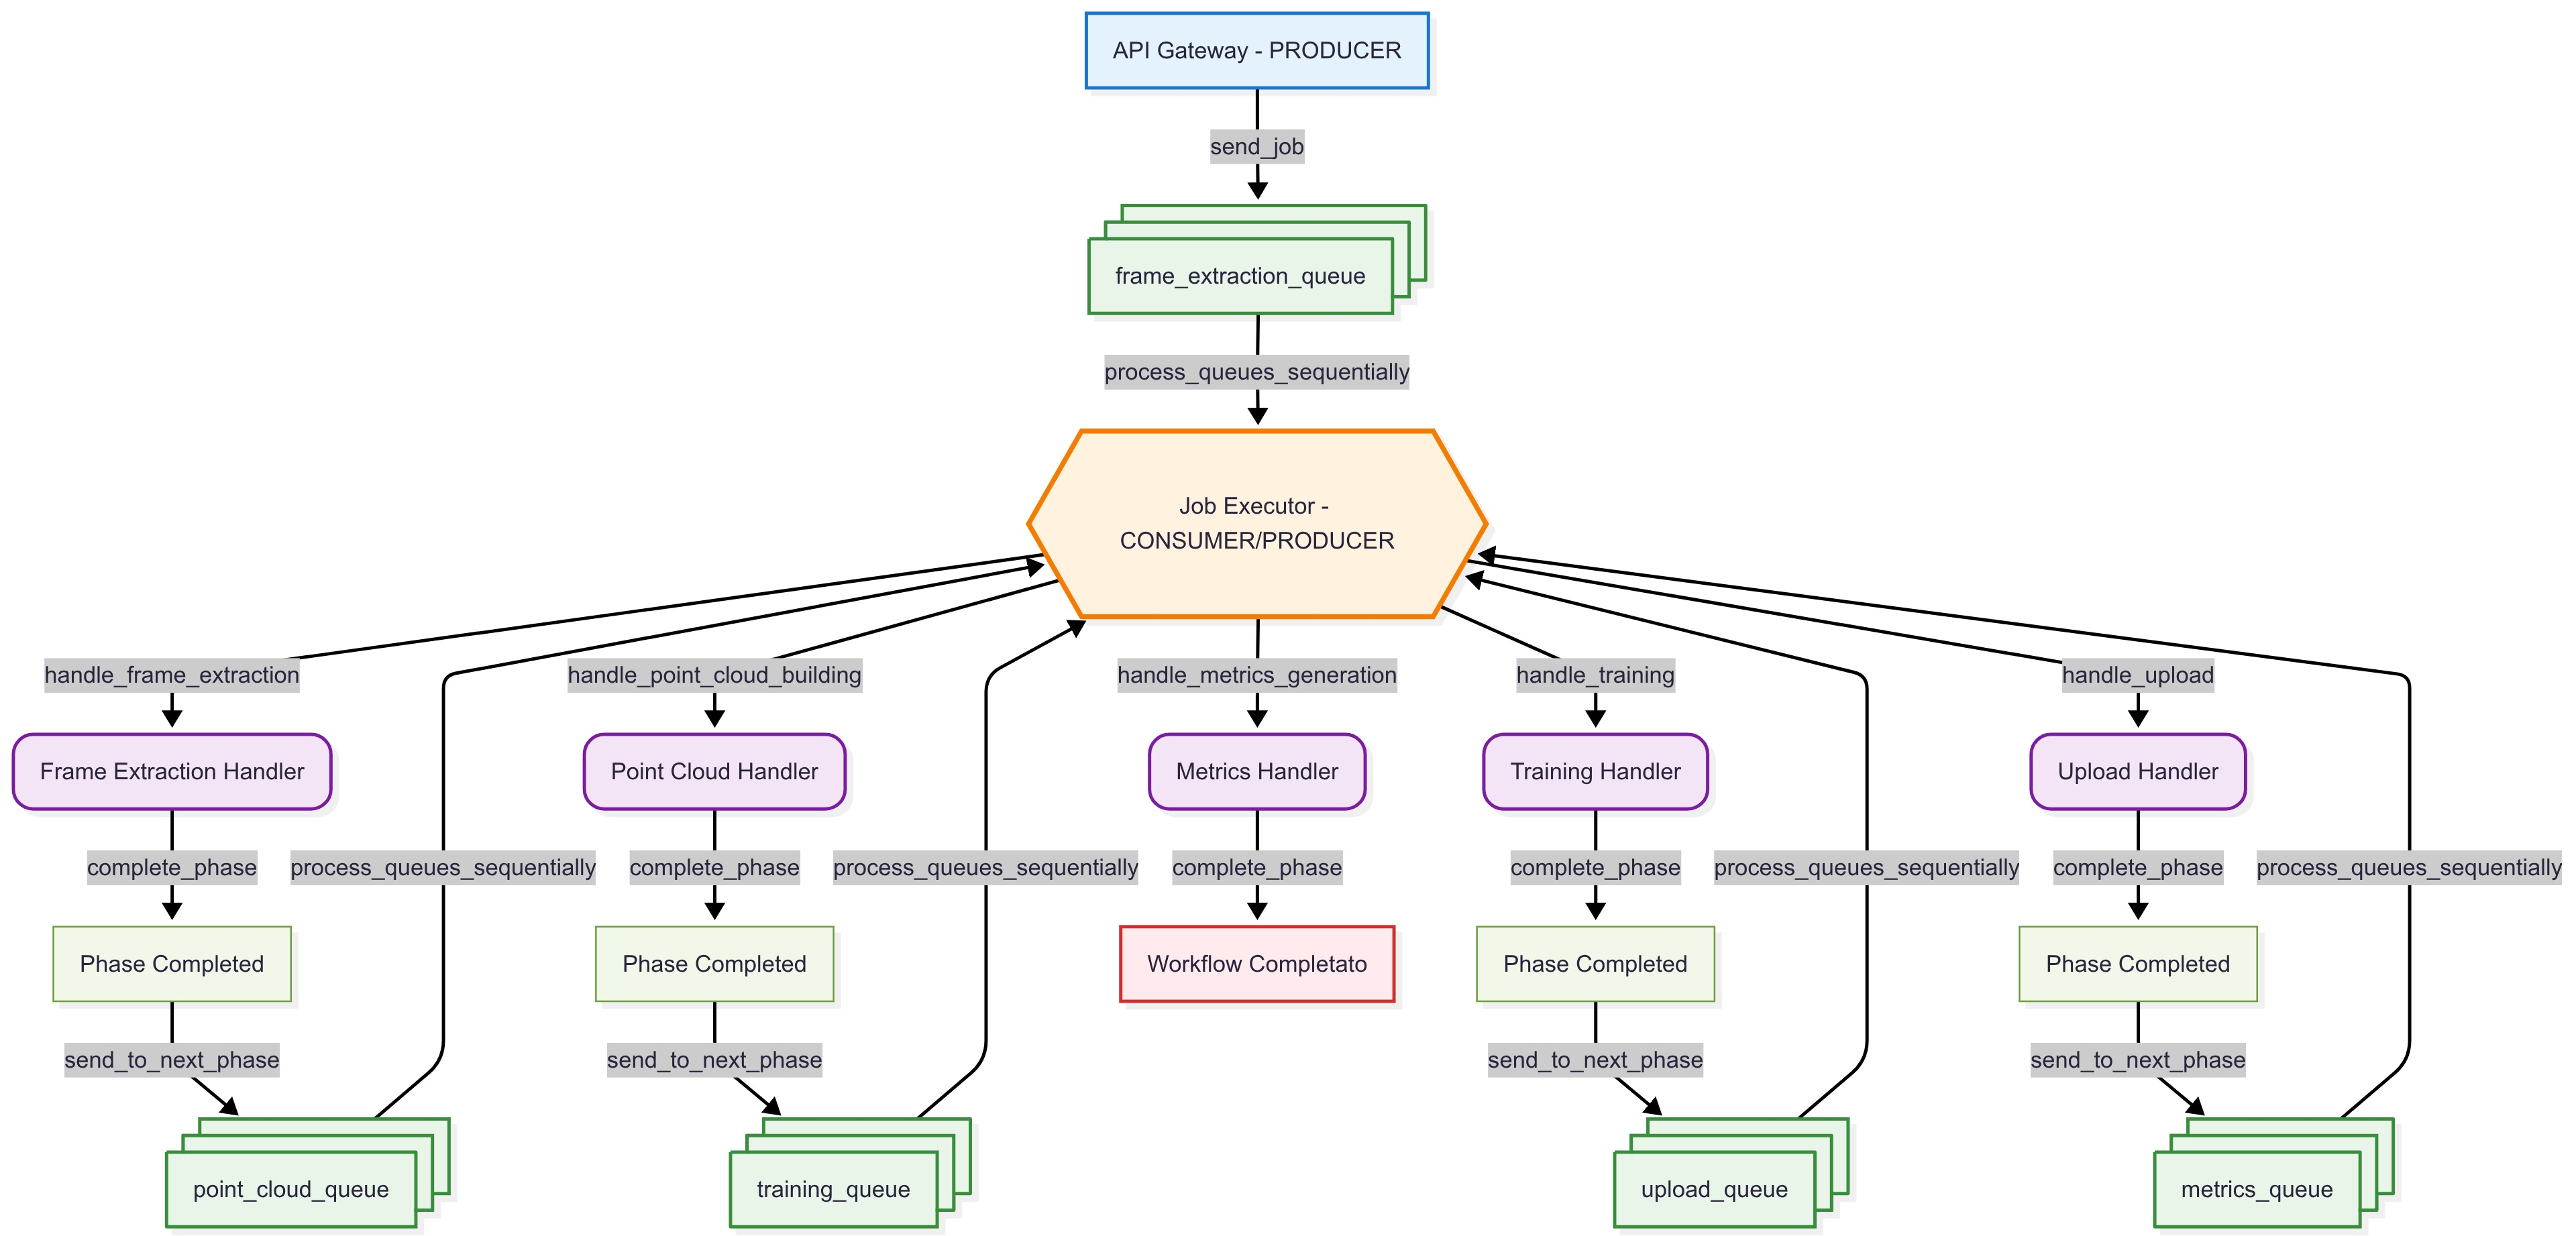
\includegraphics[width=\textwidth]{images/producer_consumer_schema.jpg}
	\caption{Schema del pattern Producer-Consumer ibrido implementato dal Job Executor}
	\label{fig:producer_consumer_schema}
\end{figure}
\newpage
\subsection{Persistenza stati intermedi}

\subsubsection{Pattern di gestione dati intermedi}

Le prime tre fasi del workflow (Frame Extraction, Point Cloud Reconstruction, Training) implementano un pattern specializzato per la gestione dei dati intermedi che abilita funzionalità avanzate di fork e retry.
\newline
Ogni fase salva i propri risultati in archivi compressi standardizzati su Amazon S3, seguendo la convenzione di denominazione \texttt{\{nome\_fase\}\_phase.zip}. Questa struttura permette il recupero selettivo di dati intermedi per operazioni di reprocessing.

\begin{lstlisting}[language=python, caption=Pattern recupero e salvataggio dati intermedi]
	# Recupero dati fase precedente
	success = phase_zip_helper.download_and_extract_phase_zip(
	phase_zip_s3_key, model_dir
	)
	
	# Salvataggio risultati fase corrente
	is_zip_uploaded = phase_zip_helper.create_phase_zip_and_upload(
	model_id, model_dir, PHASE_ZIP_NAME, ['directory_output']
	)
\end{lstlisting}

\subsubsection{Funzionalità di Fork e Retry}
Il pattern dei dati intermedi abilita la \textbf{fork e il retry di modelli} a partire da fasi intermedie, permettendo comparazioni algoritmiche e sperimentazione senza dover ripetere l'intero workflow.

\noindent Ad esempio, un utente potrebbe biforcare un modello completato almeno fino alla fase di Point Cloud Reconstruction per testare un algoritmo di training differente, riutilizzando i la point cloud già generata in precedenza e salvata come dato intermedio su S3. Questo approccio riduce significativamente i tempi di sperimentazione e ottimizza l'utilizzo delle risorse computazionali.

\subsubsection{Gestione fasi secondarie}

Tra le fasi già citate in precedenza, ci sono due fasi che seguono un pattern semplificato per il quale non serve generare dati intermedi persistenti e sono considerate \textbf{secondarie} (seppur fondamentali). Si tratta di:

\begin{itemize}
	\item \textbf{Upload modello finale}: Gestisce la preparazione e il caricamento del modello 3D per la visualizzazione, convertendo i risultati del training in formati ottimizzati per il web viewer.
	
	\item \textbf{Generazione metriche}: Calcola le metriche di qualità (PSNR, SSIM, LPIPS) confrontando rendering di test con immagini ground truth, salvando i risultati direttamente nel database.
\end{itemize}

Separando queste fasi permettiamo la visualizzazione immediata dei modelli 3D generati mentre le metriche vengono calcolate in background: questo migliora l'esperienza utente senza compromettere l'affidabilità del sistema.

\subsection{Resilienza e Fault Tolerance}

Il sistema implementa una strategia di gestione degli errori progettata per garantire continuità operativa attraverso meccanismi di isolamento e persistenza dei dati critici.

\subsubsection{Strategie di Error Handling}

Viene adottato un approccio stratificato per la gestione degli errori, implementando meccanismi di protezione a diversi livelli:

\begin{itemize}
	\item \textbf{Isolamento degli errori}: Il fallimento di un singolo job non compromette l'elaborazione di altri job nel sistema. Ogni workflow opera in modo indipendente, permettendo al sistema di continuare l'elaborazione dei job rimanenti anche in presenza di errori specifici.
	
	\item \textbf{Gestione fallimenti controllata}: Il sistema evita loop infiniti di retry confermando anche i messaggi falliti, delegando la gestione dei retry all'interfaccia utente attraverso funzionalità di restart del modello.
\end{itemize}

\subsubsection{Meccanismi di Persistenza degli Stati}

La resilienza del sistema si basa su diversi meccanismi di persistenza che garantiscono la continuità operativa:

\begin{itemize}
	\item \textbf{Checkpointing degli stati}: Il sistema implementa tracking degli stati di elaborazione attraverso aggiornamenti dei metadati in MongoDB. Il tracking avviene all'inizio e alla fine di ogni fase (\texttt{start\_phase} e \texttt{complete\_phase}), permettendo il monitoraggio del progresso e la gestione dei retry.
	
	\item \textbf{Dati intermedi persistenti}: Le fasi intermedie del workflow vengono salvate come archivi compressi su Amazon S3, abilitando funzionalità di fork e retry senza dover riprocessare l'intero pipeline.
\end{itemize}

\subsubsection{Database Monitoring}

MongoDB fornisce tracking dettagliato dello stato di ogni modello, includendo:

\begin{itemize}
	\item Progressione attraverso le fasi del workflow
	\item Tempi di elaborazione per ogni fase
	\item Metadati completi per troubleshooting e analisi delle performance
	\item Gestione degli stati di errore e recovery
\end{itemize}

Questa architettura di resilienza assicura che il sistema possa operare stabilmente, fornendo meccanismi per il recovery attraverso l'interfaccia utente e mantenendo la visibilità completa sullo stato delle elaborazioni.



\section{Layer di Pre-elaborazione}

Il Layer di Pre-elaborazione rappresenta la fase iniziale critica del workflow, responsabile della trasformazione del contenuto video di input in una rappresentazione geometrica 3D utilizzabile per il training. Questo layer combina due processi sequenziali complementari: l'estrazione intelligente di frame dal video sorgente e la ricostruzione della nuvola di punti 3D attraverso tecniche di Structure from Motion.

\subsection{Architettura del Layer}

Il Layer di Pre-elaborazione è organizzato come pipeline sequenziale che coordina due servizi specializzati:

\begin{enumerate}
	\item \textbf{Video Preprocessing Service}: Trasformazione video in dataset di frame ottimizzato
	\item \textbf{Point Cloud Reconstruction Service}: Ricostruzione geometrica 3D tramite COLMAP
\end{enumerate}

\subsubsection{Strategia di Containerizzazione Differenziata}

Il layer implementa strategie di deployment diverse per i due servizi, basate su considerazioni pragmatiche di complessità e risorse.
\newline
\newline
Il \textbf{Video Preprocessing Service} è mantenuto \textbf{all'interno del container del Job Executor}, a differenza degli altri servizi computazionali che sono containerizzati separatamente.\newpage Questa scelta deriva da valutazioni pragmatiche:

\begin{itemize}
	\item \textbf{Peso computazionale marginale}: Il preprocessing video ha durata contenuta e non impatta l'esecuzione sequenziale dei job
	\item \textbf{Dipendenze leggere}: Utilizzo di librerie esterne facilmente integrabili senza necessità di ambienti dedicati
	\item \textbf{Complessità operativa ridotta}: La separazione introdurrebbe complessità di deploy senza benefici concreti
\end{itemize}

Il \textbf{Point Cloud Reconstruction Service} è implementato come container specializzato basato su PyTorch con supporto CUDA, giustificato da:

\begin{itemize}
	\item \textbf{Complessità computazionale}: Operazioni intensive che richiedono ottimizzazioni specifiche
	\item \textbf{Dipendenze pesanti}: Integrazione di COLMAP e librerie di computer vision specializzate
	\item \textbf{Isolamento computazionale}: Necessità di ambiente dedicato per riproducibilità e gestione risorse
\end{itemize}

\subsection{Video Preprocessing Service}

Il preprocessing video è orchestrato dall'handler \texttt{handle\_frame\_extraction} che funge da punto di connessione tra il sistema di code RabbitMQ e il servizio specializzato. L'handler coordina il flusso di elaborazione delegando le operazioni atomiche al \texttt{VideoFrameExtractionService}, garantendo isolamento delle responsabilità e gestione robusta degli errori.

Il \texttt{VideoFrameExtractionService} implementa tutte le operazioni di preprocessing come servizio atomico, assicurando consistenza e tracciabilità completa del processo attraverso un'unica interfaccia pubblica \texttt{extract\_frames}.

\subsubsection{Pipeline di Preprocessing Video}


\paragraph{1) Download e Validazione}
\mbox{}\\
La pipeline inizia con il recupero del video sorgente dal storage S3 utilizzando il sistema di cache intelligente del \texttt{RepositoryService}, seguito da controlli rigorosi implementati dal metodo \texttt{\_validate\_inputs} per garantire integrità e accessibilità del file video.

\paragraph{2) Analisi Metadati Video}
Il sistema esegue un'analisi completa delle caratteristiche del video attraverso il metodo \texttt{\_analyze\_video}:

\begin{lstlisting}[language=python, caption=Analisi metadati video completa]
	def _analyze_video(self, video_path: str) -> Dict[str, Any]:
	cap = cv2.VideoCapture(video_path)
	original_width = int(cap.get(cv2.CAP_PROP_FRAME_WIDTH))
	original_height = int(cap.get(cv2.CAP_PROP_FRAME_HEIGHT))
	video_fps = cap.get(cv2.CAP_PROP_FPS)
	total_frames = int(cap.get(cv2.CAP_PROP_FRAME_COUNT))
	duration = total_frames / video_fps if video_fps > 0 else 0
	
	# Determinazione orientamento
	is_portrait = original_height > original_width
	
	return {
		'original_width': original_width,
		'original_height': original_height,
		'video_fps': video_fps,
		'duration_seconds': duration,
		'is_portrait': is_portrait,
		'orientation': 'Portrait' if is_portrait else 'Landscape'
	}
\end{lstlisting}

\paragraph{3) Adattamento Orientamento}
Una delle ottimizzazioni più importanti riguarda la gestione intelligente dell'orientamento video:

\begin{lstlisting}[language=python, caption=Logica di adattamento orientamento]
	# Per portrait, target_height diventa la width effettiva
	final_width = target_height if is_portrait else target_width
\end{lstlisting}

I parametri di qualità sono configurati assumendo orientamento landscape standard. Per video portrait, il sistema utilizza \texttt{target\_height} come dimensione principale per mantenere la qualità visiva desiderata.

\paragraph{4) Calibrazione FPS per Target Frame}
Il cuore del preprocessing è la calibrazione intelligente del frame rate di estrazione:

\begin{lstlisting}[language=python, caption=Algoritmo di calibrazione FPS]
	if duration > 0:
		extraction_fps = target_frame_count / duration
		extraction_fps = min(extraction_fps, video_fps)  # Vincolo hardware
		extraction_fps = max(0.5, extraction_fps)        # Soglia qualità minima
	else:
		extraction_fps = 1.0  # Fallback sicuro
\end{lstlisting}

Sebbene il numero di frame target sia teoricamente parametrizzabile attraverso il sistema di parametrizzazione adattiva, la configurazione attuale fissa questo valore a 200 frame, identificato come ottimale per bilanciare qualità della ricostruzione e efficienza computazionale.

\paragraph{5) Estrazione Frame con Sharp-Frames}
L'estrazione utilizza il tool specializzato Sharp-Frames con configurazione ottimizzata per la pipeline COLMAP:

\begin{lstlisting}[language=python, caption=Configurazione Sharp-Frames ottimizzata]
	cmd = [
	"sharp-frames",
	video_path,
	output_directory,
	"--selection-method", "best-n",
	"--min-buffer", "1",
	"--fps", str(optimized_params['extraction_fps'])
	]
	
	# Aggiunta parametro width se necessario
	final_width = optimized_params.get('final_width')
	if final_width is not None:
	cmd.extend(["--width", str(final_width)])
\end{lstlisting}

La scelta del metodo \texttt{best-n} prioritizza la qualità dei singoli frame, aspetto critico per il successo delle fasi successive di feature matching in COLMAP.

\paragraph{6) Finalizzazione e Persistenza}
Il processo conclude con validazione output, generazione thumbnail per il layer di presentazione, creazione archivio fase per supportare fork/retry, e generazione metadati dettagliati per tracciabilità completa.

\begin{figure}[htbp]
	\centering
	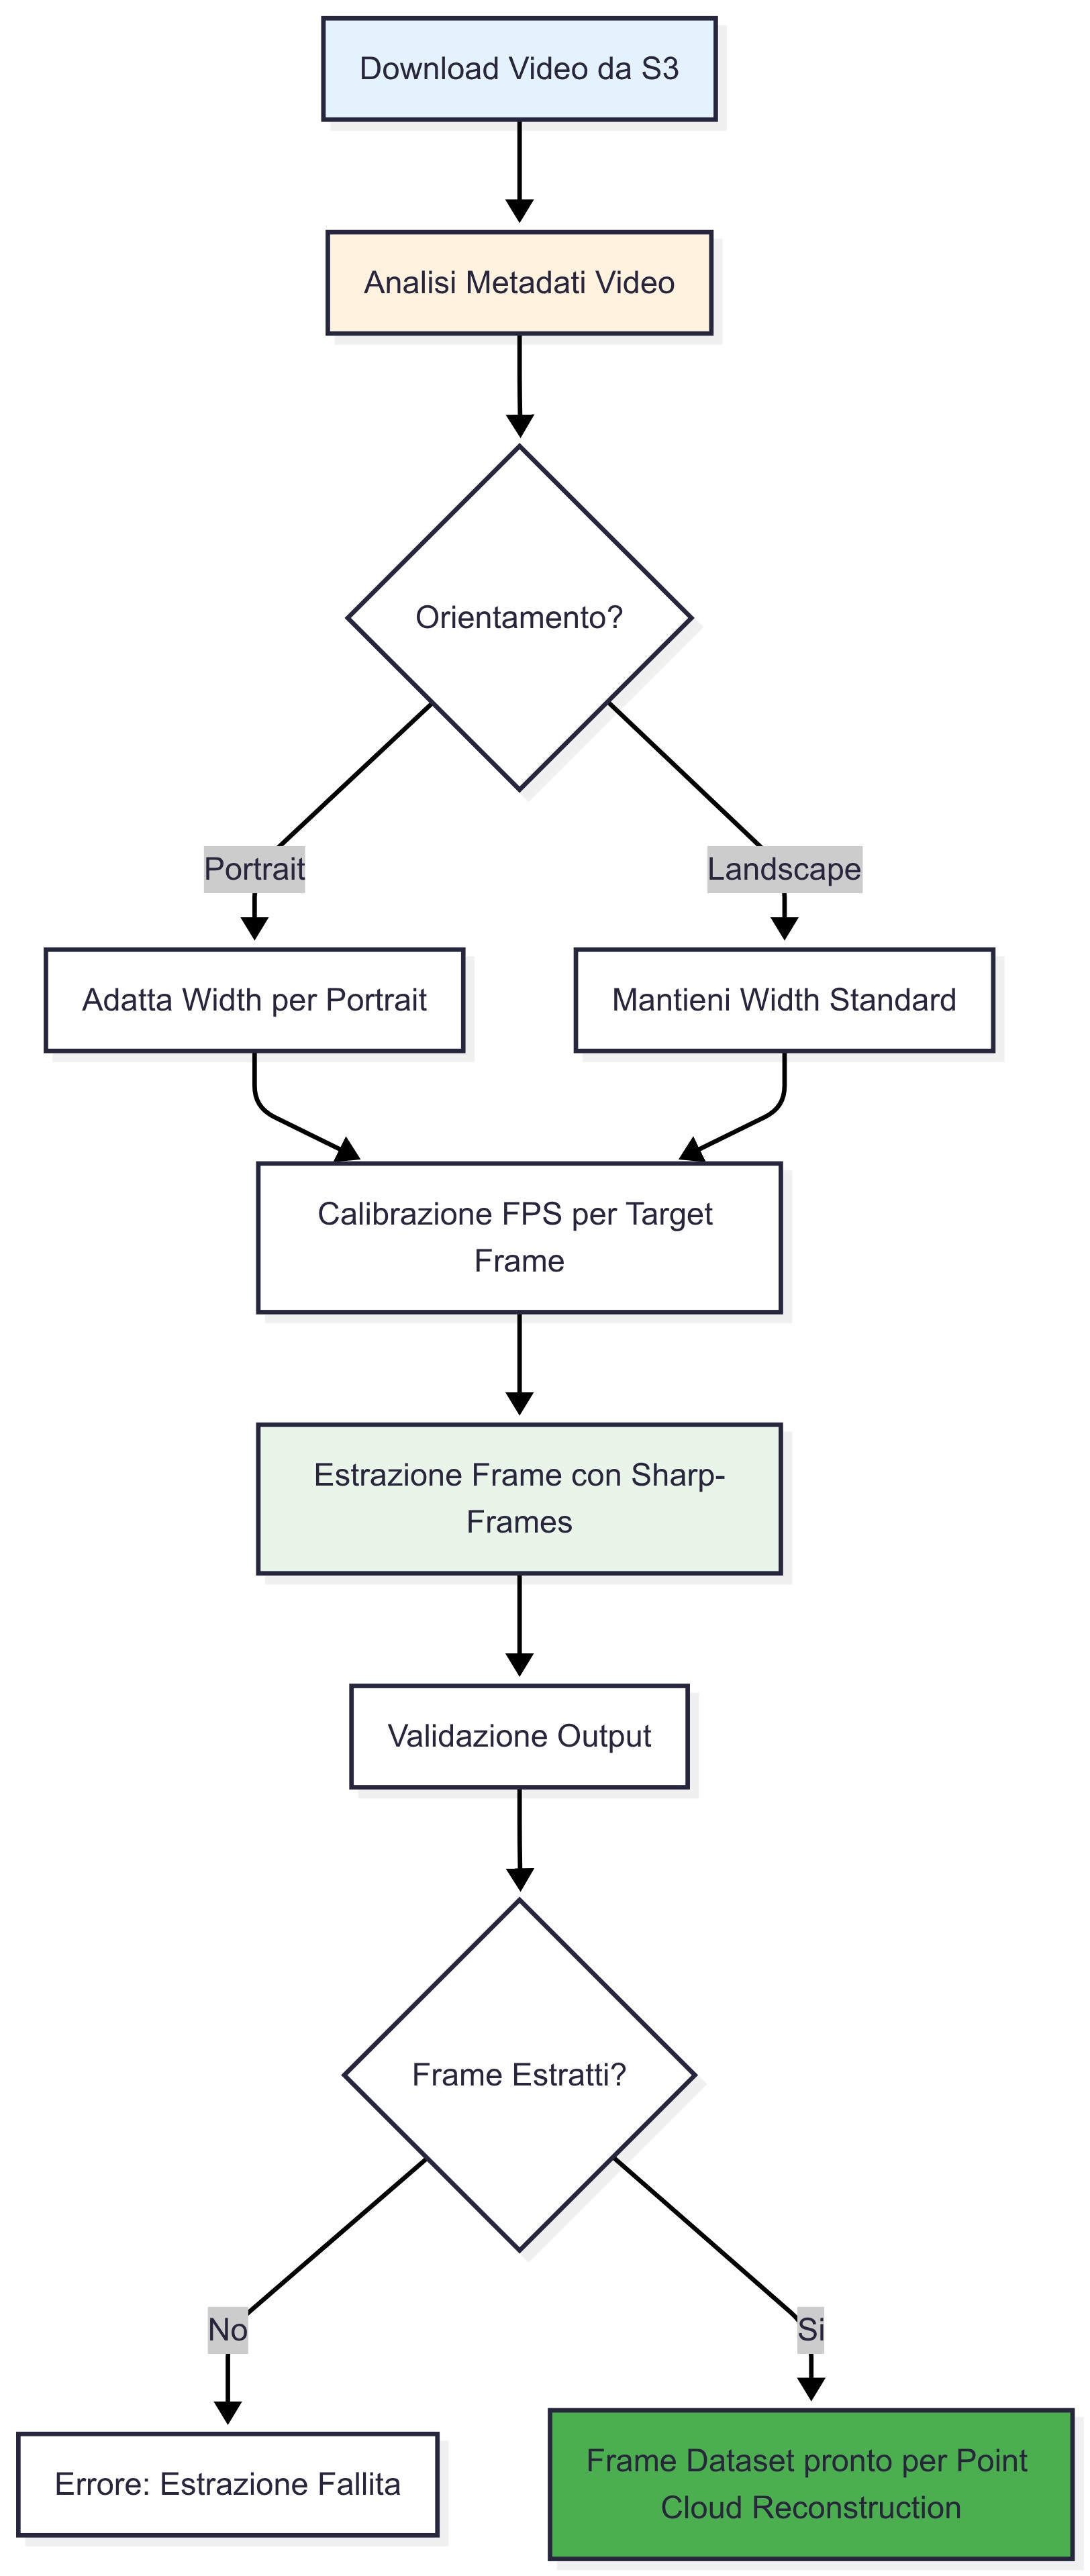
\includegraphics[width=0.6\textwidth]{images/frame_extraction_diagram.jpg}
	\caption{Schema del estrazione frames da video}
	\label{fig:frame_extraction_diagram}
\end{figure}
\newpage
\subsection{Point Cloud Reconstruction Service}

\subsubsection{Handler Point Cloud Building}
La Point Cloud Reconstruction è orchestrata dall'handler \texttt{handle\_point\_cloud\_building} che coordina la ricostruzione della nuvola di punti 3D a partire dal dataset di frame ottimizzato.

\paragraph{Recupero Dataset e Validazione}
Il sistema recupera il dataset di frame dalla fase precedente, gestendo automaticamente diverse fonti tramite il pattern di dati intermedi.

\paragraph{Generazione Point Cloud via COLMAP}
La ricostruzione avviene tramite chiamata al servizio COLMAP containerizzato con analisi automatica della strategia ottimale:

\begin{lstlisting}[language=python, caption=Generazione point cloud con monitoraggio performance]
	sparse_dir = os.path.join(model_dir, 'sparse')
	
	colmap_start_time = datetime.utcnow()
	
	# COLMAP API call con analisi automatica strategia
	convert_request = {"input_dir": model_dir}
	response = requests.post(COLMAP_API_URL + "/convert", json=convert_request)
	
	colmap_duration_seconds = (datetime.utcnow() - colmap_start_time).total_seconds()
	
	# Verifica output e raccolta statistiche
	generated_points = job_utils.get_colmap_reconstruction_stats(model_dir)
\end{lstlisting}

\subsubsection{Strategie di Feature Matching: Analisi Comparativa}

\begin{itemize}
\item \textbf{Exhaustive Matching}: la strategia exhaustive confronta ogni immagine con tutte le altre nel dataset, con \textbf{complessità O(n²)}. Garantisce qualità massima per dataset fino a diverse centinaia di immagini, ha tempi di elaborazione che variano da 2 a 5 minuti per scene rappresentate da circa 200 immagini a seconda della loro complessità.

\item \textbf{Sequential Matching}:
la strategia sequential sfrutta l'ordine temporale dei frame video, con \textbf{complessità O(n × overlap)}. Offre efficienza temporale significativa ma produce point cloud meno dense che richiedono maggiore sforzo durante le fasi di pruning e densification del training Gaussian Splatting.

\item \textbf{Vocabulary Tree Matching}:
la strategia vocabulary tree utilizza un albero di vocabolario precompilato, con \textbf{complessità O(n log n)}. È ottimale per grandi dataset (migliaia di immagini) e offre una qualità molto vicina a quella dela strategia exhaustive quando la quantità di feature media è bassa.
\end{itemize}	
\subsubsection{Pipeline di Ricostruzione Ottimizzata}

Il processo include feature extraction parametrizzata, bundle adjustment ottimizzato con tolleranze specifiche, e generazione di statistiche dettagliate per tracciabilità e debugging.

\subsection{Integrazione e Coordinamento}

\subsubsection{Flusso di Dati tra Servizi}

Il layer implementa un flusso di dati efficiente attraverso il pattern di archivi intermedi:

\begin{enumerate}
	\item \textbf{Video Preprocessing}: Genera archivio \texttt{point\_cloud\_building\_phase.zip} contenente frame estratti
	\item \textbf{Point Cloud Reconstruction}: Consuma frame e genera archivio \texttt{training\_phase.zip} con nuvola di punti
	\item \textbf{Handoff al Training}: Fornisce dataset completo per gli algoritmi Gaussian Splatting
\end{enumerate}

\subsubsection{Gestione Metadati e Performance}

Entrambi i servizi generano metadati dettagliati che documentano:

\begin{itemize}
	\item \textbf{Parametri di elaborazione}: Configurazioni utilizzate per riproducibilità
	\item \textbf{Statistiche quantitative}: Conteggi frame, punti 3D generati, tempi di elaborazione
	\item \textbf{Performance data}: Metriche per analisi e ottimizzazioni future
	\item \textbf{Versioning}: Tracciabilità delle versioni software utilizzate
\end{itemize}

Il Layer di Pre-elaborazione rappresenta quindi un componente critico e sofisticato che, attraverso l'integrazione intelligente di algoritmi di preprocessing video e ricostruzione geometrica 3D, trasforma contenuti video grezzi in rappresentazioni geometriche ottimizzate per il training Gaussian Splatting, garantendo qualità, efficienza e tracciabilità completa del processo.

\section{Layer di Training}

Il motore di training rappresenta il cuore computazionale del sistema, responsabile dell'esecuzione degli algoritmi di Gaussian Splatting. L'implementazione adotta un approccio containerizzato che isola ogni algoritmo in un ambiente dedicato, esponendo le funzionalità attraverso API REST standardizzate.

\subsection{Architettura containerizzata multi-algoritmo}

Il sistema implementa tre container specializzati, ciascuno dedicato a un algoritmo specifico:

\begin{itemize}
	\item \textbf{gaussian-splatting}: Implementazione di riferimento del paper originale
	\item \textbf{3dgs-mcmc}: Variante con campionamento MCMC per ottimizzazione stocastica  
	\item \textbf{taming-3dgs}: Versione ottimizzata per scene complesse
\end{itemize}

Ogni container segue una strategia di build multi-stage per ottimizzare le dimensioni e i tempi di compilazione:

\subsection{Handler Training}

L'handler di training coordina l'esecuzione degli algoritmi di Gaussian Splatting, gestendo la configurazione dei parametri e le funzionalità specifiche come la depth regularization per il motore standard.

\subsubsection{Recupero Dataset e Configurazione}

Il sistema recupera la point cloud e le immagini processate dalla fase precedente, configurando dinamicamente i parametri in base all'algoritmo selezionato:

\begin{lstlisting}[language=python, caption=Inizializzazione e configurazione training]
	model_service.start_phase(model_id, "training")
	model = model_service.get_model_by_id(model_id)
	
	model_dir = os.path.join(WORKING_DIR, f"{model_id}")
	image_dir = os.path.join(model_dir, "images")
	sparse_dir = os.path.join(model_dir, "sparse")
	
	# Recupera ZIP dalla fase point cloud building se necessario
	if not (os.path.exists(image_dir) and os.path.exists(sparse_dir)):
	training_zip_s3_key = f"{S3_STAGING_PREFIX}/{model.parent_model_id}/{TRAINING_PHASE_ZIP_NAME}"
	success = phase_zip_helper.download_and_extract_phase_zip(
	training_zip_s3_key, model_dir
	)
	
	# Configurazione parametri tramite TrainingParamsService
	engine = model.training_config.get('engine')
	quality_level = model.training_config.get('quality_level')
	
	generated_params = training_params_service.generate_params(
	Engine(engine), QualityLevel(quality_level)
	)
\end{lstlisting}

\subsubsection{Depth Regularization per Gaussian Splatting standard}

Per il motore \textit{Gaussian Splatting} standard, viene implementata una fase di \textbf{depth regularization}, come suggerito dalla documentazione ufficiale, al fine di migliorare la qualità della ricostruzione nelle scene real-world.
Questa tecnica vincola le gaussiane a disporsi lungo superfici coerenti con le stime di profondità ottenute dalle immagini, riducendo la presenza di artefatti e gaussiane fluttuanti nello spazio 3D, tipiche delle scene acquisite dal mondo reale.

Nel caso delle varianti \textbf{MCMC} e \textbf{Taming}, invece, non viene impiegata depth regularization esplicita.
Queste versioni adottano strategie di ottimizzazione alternative — rispettivamente, tramite sampling stocastico e controlli specifici sulla crescita e la fusione delle gaussiane — che mitigano la formazione di outlier e favoriscono la distribuzione regolare delle gaussiane nello spazio, rendendo la regularizzazione sulla profondità meno necessaria.

È importante sottolineare che la presenza della depth regularization, pur migliorando la plausibilità geometrica della scena, \textbf{può in alcuni casi limitare le performance su metriche quantitative come il PSNR}, poiché impone vincoli aggiuntivi rispetto all’ottimizzazione puramente basata sulla ricostruzione delle immagini.

\begin{lstlisting}[language=python, caption=Endpoint depth regularization]
	@app.post("/depth_regularization")
	async def make_depth_regularization(request: DepthRegularizationRequest):
	logger.info(f"Starting depth generation - Input directory: {request.input_dir}")
	
	images_dir = os.path.join(request.input_dir, 'images')
	depths_dir = os.path.join(request.input_dir, 'depths')
	
	# STEP 1: Genera depth maps con Depth Anything V2
	depth_command = (
	f"cd /workspace/Depth-Anything-V2 && "
	f"python3 run.py --encoder vitl --pred-only --grayscale "
	f"--img-path {images_dir} --outdir {depths_dir}"
	)
	
	# Esecuzione depth generation con logging multi-thread
	depth_process = subprocess.Popen(
	depth_command, shell=True, stdout=subprocess.PIPE, 
	stderr=subprocess.PIPE, text=True, bufsize=1
	)
	
	# [Thread management per logging real-time]
	
	# STEP 2: Genera depth_params.json con scaling automatico
	params_command = (
	f"python3 /workspace/gaussian-splatting/utils/make_depth_scale.py "
	f"--base_dir {request.input_dir} --depths_dir {depths_dir}"
	)
	
	# [Esecuzione simile con thread management]
	
	return {
		"message": "Depth generation and params completed successfully",
		"depth_maps_count": depth_count,
		"depth_maps_dir": depths_dir
	}
\end{lstlisting}

\subsubsection{Esecuzione Training}

Il sistema seleziona dinamicamente l'API dell'engine containerizzato corrispondente e avvia il processo di training:

\begin{lstlisting}[language=python, caption=Esecuzione training con engine selezionato]
	# Selezione API engine dalla mappatura
	api_url = engine_map.get(engine, {}).get('api-url')
	if not api_url:
	self.fail(model_id, "training", f"Error: No api url found for engine {engine}")
	return False
	
	# Costruzione richiesta di training
	train_request = {
		"input_dir": model_dir,
		"output_dir": train_output_folder,
		"params": generated_params.final_params,  # Parametri ottimizzati
	}
	
	print(f"🎯 Starting training with engine: {engine}")
	training_start_time = datetime.utcnow()
	
	# Chiamata API training containerizzato
	response = requests.post(f"{api_url}/train", json=train_request)
	
	training_end_time = datetime.utcnow()
	training_duration = training_end_time - training_start_time
	training_duration_seconds = training_duration.total_seconds()
	
	if response.status_code != 200:
	self.fail(model_id, "training", f"Training failed: {response.text}")
	return False
\end{lstlisting}

\subsubsection{Finalizzazione e Metadati}

La fase si conclude con l'aggiornamento dei metadati, includendo statistiche di performance e informazioni sulla depth regularization:

\begin{lstlisting}[language=python, caption=Finalizzazione training con metadati estesi]
	# Aggiorna metadati con statistiche complete
	phase_metadata = {
		"training_duration_seconds": round(training_duration_seconds, 2),
		"depth_regularization_seconds": round(depth_duration_seconds, 2),
		"training_start_time": training_start_time.isoformat(),
		"training_end_time": training_end_time.isoformat(),
		"training_parameters": {
			"engine": engine,
			"quality_level": quality_level,
			"final_params": generated_params.final_params,
			"depth_regularization_enabled": engine == Engine.INRIA.value
		}
	}
	
	model_service.complete_phase(model_id, "training", metadata=phase_metadata)
\end{lstlisting}

\subsection{Interfaccia API REST unificata}

\subsubsection{Standardizzazione degli endpoint}

Ogni container espone un'interfaccia REST standardizzata che astrae le specificità implementative degli algoritmi sottostanti:

\begin{lstlisting}[language=python, caption=Definizione modelli dati per API REST]
	from fastapi import FastAPI, HTTPException
	from pydantic import BaseModel, Field
	import subprocess
	import threading
	import queue
	import logging
	from typing import Dict, Any
	
	app = FastAPI()
	
	class TrainRequest(BaseModel):
	input_dir: str  
	output_dir: str
	params: Dict[str, Any] = Field(
	default_factory=dict, 
	description="Parametri specifici dell'algoritmo"
	)
	
	class RenderRequest(BaseModel):
	output_dir: str  
	
	class MetricsRequest(BaseModel):
	output_dir: str
	
	class DepthRegularizationRequest(BaseModel):
	input_dir: str
\end{lstlisting}

\subsubsection{Gestione parametri dinamica}

La gestione dei parametri di training è implementata attraverso un sistema dinamico che costruisce automaticamente gli argomenti della command line:

\begin{lstlisting}[language=python, caption=Costruzione dinamica comando di training]
	@app.post("/train")
	async def run_train(request: TrainRequest):
	logger.info(f"Starting training - Input: {request.input_dir}")
	
	# Costruzione dinamica del comando
	command = ["python3", "/workspace/gaussian-splatting/train.py"]
	depths_dir = os.path.join(request.input_dir, 'depths')
	
	# Parametri obbligatori con depth regularization
	command.extend([
	"--resolution", "1",
	"-s", request.input_dir,
	"-m", request.output_dir,
	"-d", depths_dir  # Directory depth maps per regularization
	])
	
	# Parametri dinamici dall'utente
	boolean_flags = {"eval"}
	
	for param_key, value in request.params.items():
		if param_key in boolean_flags:
			if value:
				command.append(f"--{param_key}")
			elif param_key != 'resolution':
				command.extend([f"--{param_key}", str(value)])
	
	# Flag antialiasing automatico
	command.append(f"--antialiasing")
	
	# Esecuzione con logging real-time multi-thread
	# [Implementazione gestione processo e thread]
\end{lstlisting}

\subsubsection{Endpoint Specializzati}

Oltre al training principale, ogni container espone endpoint per le fasi complementari del workflow:

\begin{itemize}
	\item \textbf{\texttt{/train}}: Esecuzione dell'algoritmo di training principale
	\item \textbf{\texttt{/render}}: Generazione delle immagini di test per validazione
	\item \textbf{\texttt{/metrics}}: Calcolo delle metriche di qualità (PSNR, SSIM, LPIPS)
	\item \textbf{\texttt{/depth\_regularization}}: Generazione depth maps (solo gaussian-splatting standard)
\end{itemize}

\subsection{Handler Metrics Generation}
L'handler di metrics generation rappresenta la fase finale del workflow, responsabile della valutazione quantitativa del modello addestrato attraverso metriche standard di qualità visiva. Come per l'upload, questa fase è stata isolata strategicamente per permettere al modello di essere disponibile per il rendering mentre le metriche vengono calcolate in background.
\subsubsection{Inizializzazione e Validazione Output}
Il sistema verifica la disponibilità dell'output di training e prepara l'ambiente per la generazione delle metriche di valutazione:
\begin{lstlisting}[language=python, caption=Inizializzazione e validazione output training]
	model_service.start_phase(model_id, "metrics_evaluation")
	model = model_service.get_model_by_id(model_id)
	model_dir = os.path.join(WORKING_DIR, f"{model_id}")
	Verifica esistenza output del training
	output_dir = os.path.join(model_dir, 'output')
	if not os.path.exists(output_dir):
	self.fail(model_id, "metrics_evaluation", f"No folder output found")
	return False
	engine = model.training_config.get('engine', 'INRIA')
\end{lstlisting}
\subsubsection{Generazione render e calcolo metriche}
Il sistema utilizza lo stesso engine containerizzato del training per generare render di valutazione e calcolare le metriche standard di qualità visiva (SSIM, PSNR, LPIPS):
\begin{lstlisting}[language=python, caption=Generazione render e calcolo metriche]
	engine = model.training_config.get('engine', 'INRIA')
	Generazione render per valutazione
	render_request = {"output_dir": output_dir}
	response = requests.post(engine_map.get(engine).get('api-url') + "/render", json=render_request)
	response.raise_for_status()
	Calcolo metriche di qualità
	metrics_request = {"output_dir": output_dir}
	response = requests.post(engine_map.get(engine).get('api-url') + "/metrics", json=metrics_request)
	response.raise_for_status()
	Verifica generazione del file risultati
	results_json_path = os.path.join(output_dir, "results.json")
	if not os.path.exists(results_json_path):
	raise FileNotFoundError("Il file 'results.json' non è stato trovato.")
	with open(results_json_path, 'r') as f:
	results_data = json.load(f)
\end{lstlisting}
\newpage
\subsubsection{Finalizzazione e Persistenza Metriche}
La fase si conclude con la persistenza delle metriche calcolate nei metadati del modello, rendendo immediatamente disponibili per visualizzazione nel frontend:
\begin{lstlisting}[language=python, caption=Persistenza metriche e completamento workflow]
	Salvataggio metriche nei metadati del modello
	model_service.complete_phase(
	model_id,
	"metrics_evaluation",
	overall_status="COMPLETED",
	metadata={"metrics": results}
	)
	print(f"✅ Metriche generate e salvate per model {model_id}")
\end{lstlisting}

La gestione intelligente delle chiavi del file JSON è fondamentale perché il nome delle sezioni include il numero di iterazioni specificato nella parametrizzazione (es. \texttt{ours\_30000} per 30.000 iterazioni). Questo collegamento diretto tra parametri di training e struttura delle metriche garantisce che la valutazione sia sempre coerente con la configurazione utilizzata per l'addestramento. L'isolamento di questa fase permette all'utente di visualizzare il modello 3D immediatamente dopo l'upload, mentre le metriche vengono calcolate in background e aggiornate progressivamente nell'interfaccia.

\section{Layer Backend-for-Frontend}

\subsection{Architettura e Funzionalità Principali}

Il layer Backend-for-Frontend (API Gateway) funge da punto di accesso unico e sicuro per tutte le operazioni sui modelli 3D, orchestrando la comunicazione tra frontend, database MongoDB, sistema di code RabbitMQ e storage S3 (Fig. \ref{fig:bff_architecture}).

\begin{figure}[H]
	\centering
	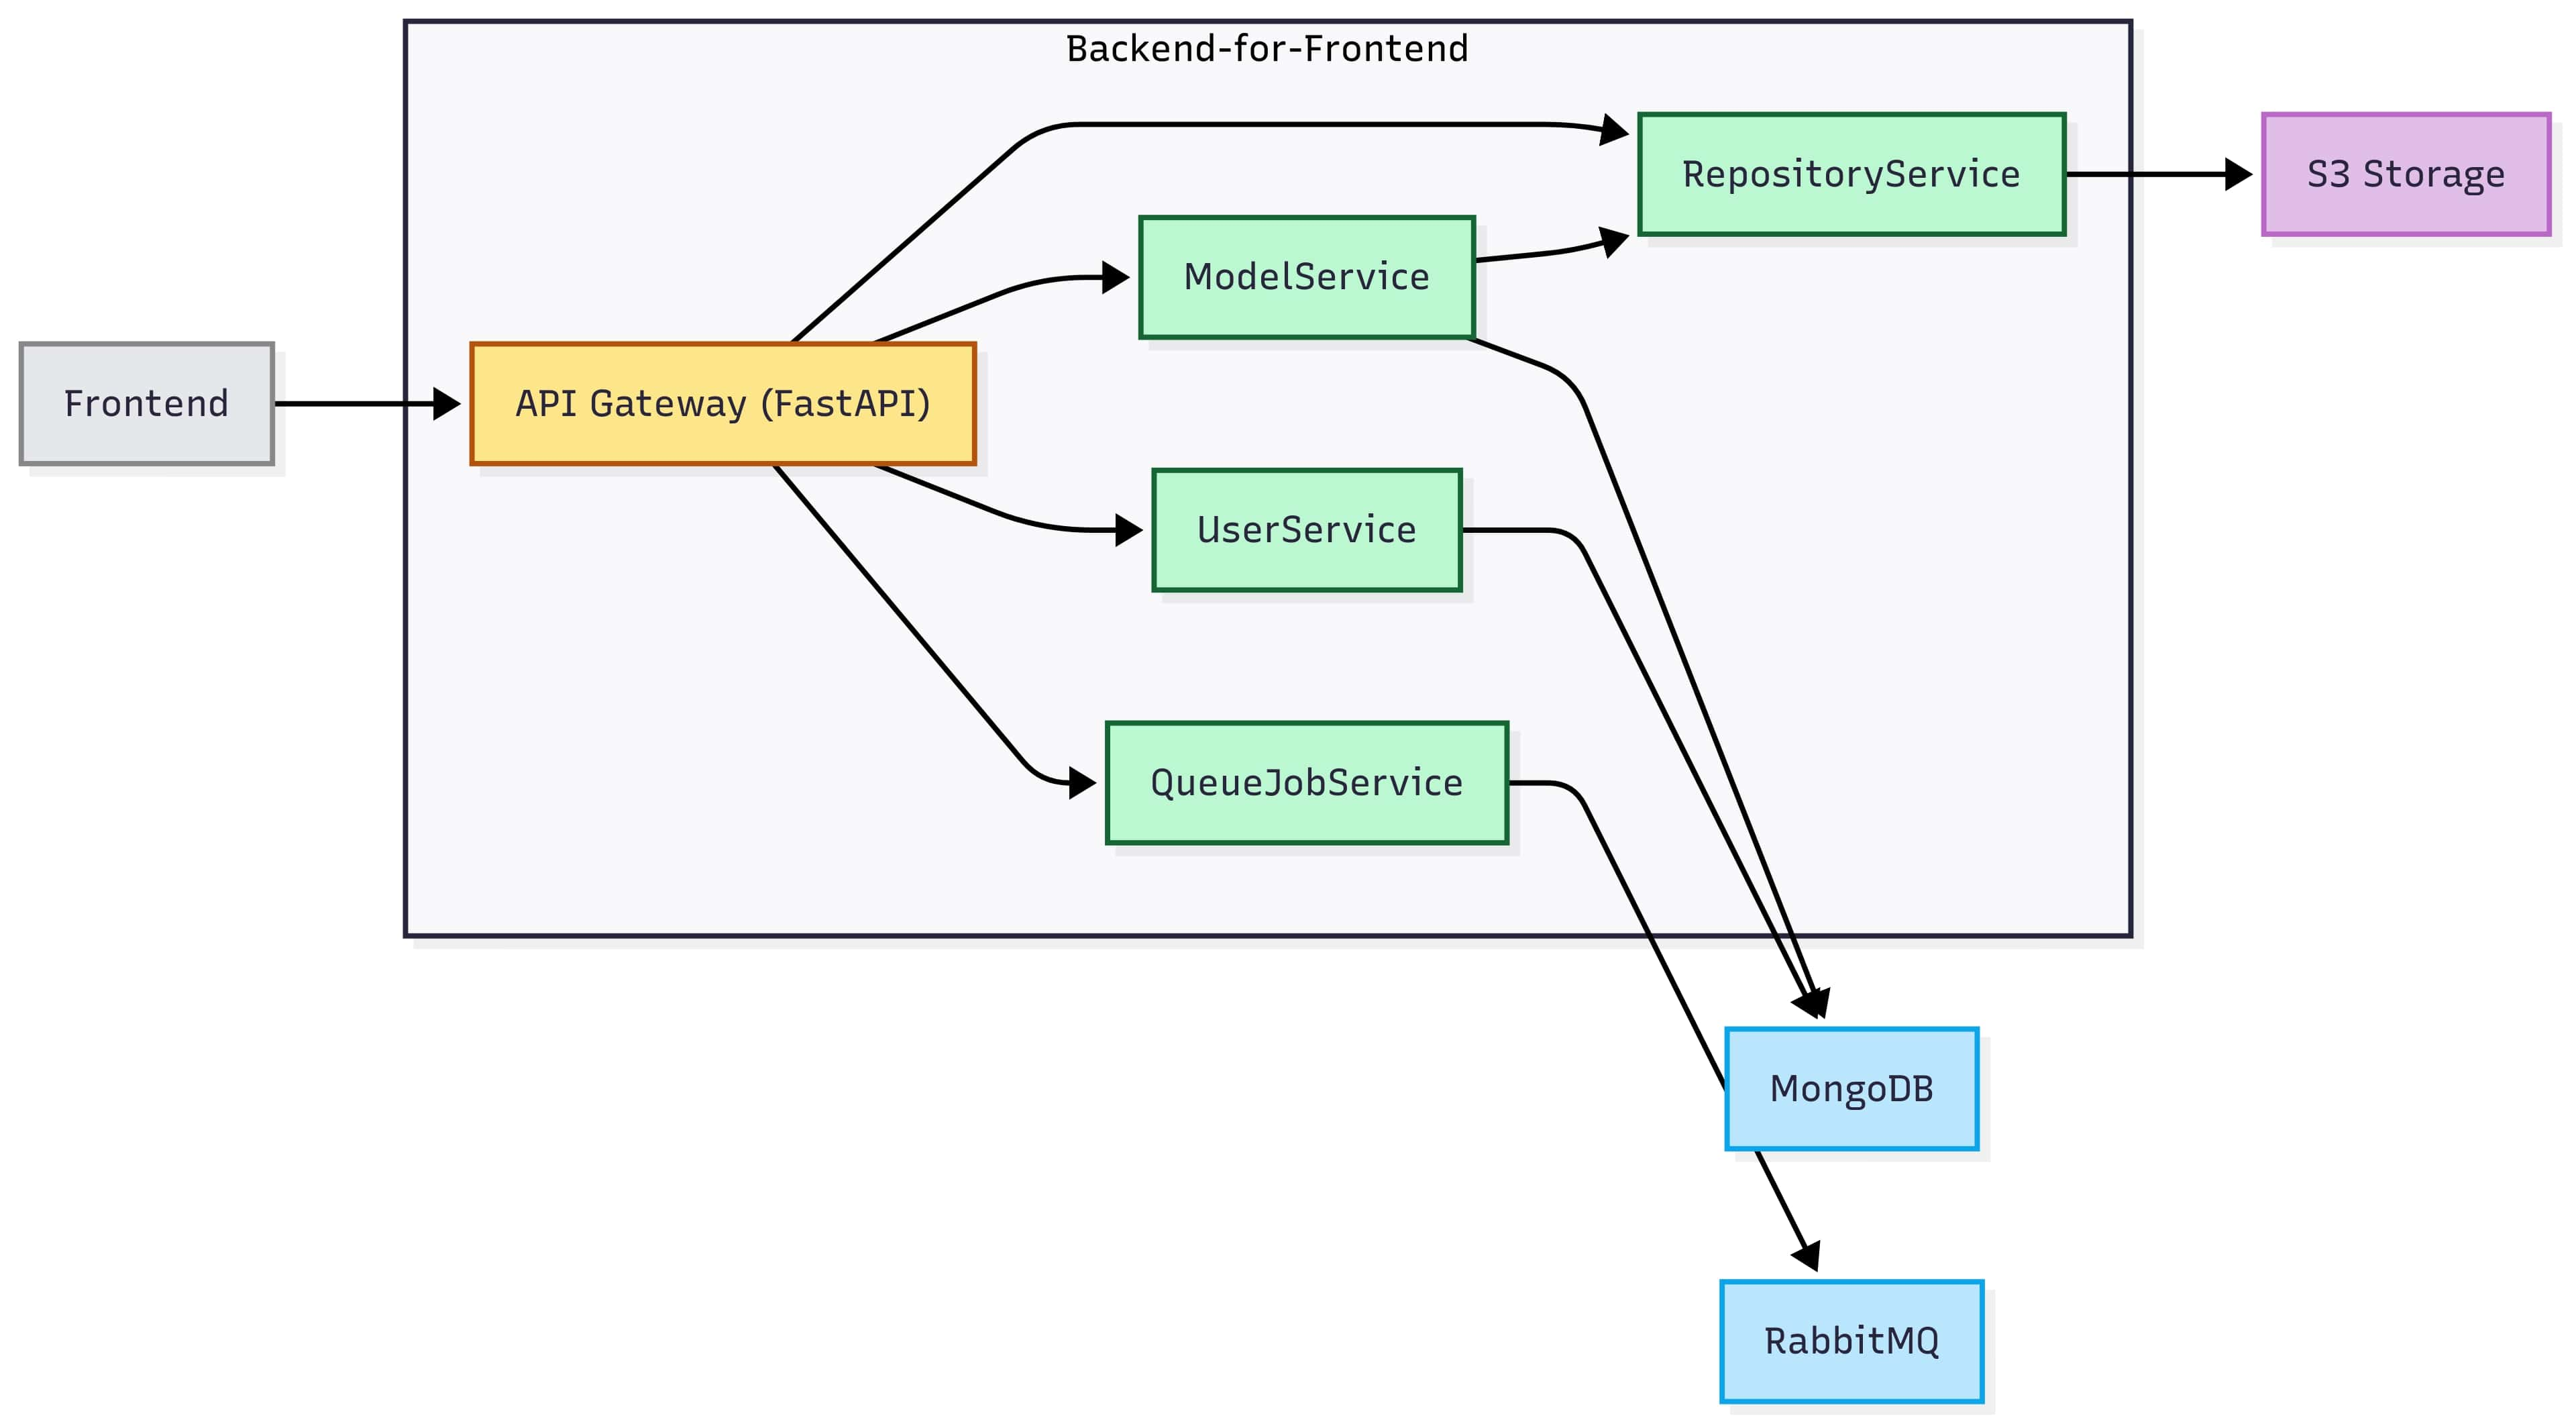
\includegraphics[width=0.9\textwidth]{images/bff_architecture.jpg}
	\caption{Architettura del layer Backend-for-Frontend}
	\label{fig:bff_architecture}
\end{figure}

\subsection{Riepilogo Endpoint REST e WebSocket}

La Tabella~\ref{tab:endpoint_bff} riepiloga i principali endpoint esposti dall'API Gateway.

\begin{table}[H]
	\centering
	\begin{tabular}{|l|l|l|l|}
		\hline
		Metodo & Endpoint & Descrizione & Autenticazione \\
		\hline
		POST & /register & Registrazione utente admin & Basic Auth \\
		POST & /token & Login e rilascio JWT & Nessuna \\
		POST & /models/ & Creazione nuovo modello & Basic Auth \\
		GET & /models/ & Elenco modelli & Basic Auth \\
		GET & /models/\{id\} & Dettaglio modello & Basic Auth \\
		POST & /models/\{id\}/retry & Retry modello fallito & Basic Auth \\
		DELETE & /models/\{id\} & Eliminazione modello & Basic Auth \\
		POST & /s3/upload-url/ & Generazione presigned URL S3 & Basic Auth \\
		GET & /health & Health check API & Nessuna \\
		WS & /ws/notifications & Notifiche real-time & -- \\
		\hline
	\end{tabular}
	\caption{Principali endpoint esposti dall’API Gateway}
	\label{tab:endpoint_bff}
\end{table}

\subsection{Logica e Flussi Principali degli Endpoint}

\subsubsection{Registrazione e Autenticazione}

\begin{itemize}
	\item \textbf{Registrazione} (\texttt{POST /register}): Consente la creazione di nuovi utenti admin, protetta tramite HTTP Basic Authentication.
	\item \textbf{Login} (\texttt{POST /token}): Permette agli utenti di autenticarsi tramite username e password e ricevere un JWT per l’accesso alle altre API.
\end{itemize}

\subsubsection{Gestione Modelli 3D}

\begin{itemize}
	\item \textbf{Creazione modello} (\texttt{POST /models/}): Permette la creazione di un nuovo modello 3D (ex novo o fork). Il servizio:
	\begin{enumerate}
		\item Valida la richiesta e crea il modello su MongoDB.
		\item Invia un job di elaborazione su RabbitMQ.
		\item Restituisce le informazioni del nuovo modello.
	\end{enumerate}
	\item \textbf{Elenco modelli} (\texttt{GET /models/}): Restituisce una lista di modelli 3D con supporto a paginazione, filtri (per nome e stato) e ordinamento.
	\item \textbf{Dettaglio modello} (\texttt{GET /models/\{id\}}): Recupera tutti i dettagli di un modello tramite il suo identificatore unico.
	\item \textbf{Retry modello} (\texttt{POST /models/\{id\}/retry}): Permette di riavviare l’elaborazione di un modello che ha subito un errore in una delle fasi.
	\item \textbf{Eliminazione modello} (\texttt{DELETE /models/\{id\}}): Consente di rimuovere un modello dal database (implementazione futura).
\end{itemize}

\subsubsection{Gestione Upload Video}

\begin{itemize}
	\item \textbf{Generazione presigned URL} (\texttt{POST /s3/upload-url/}): Genera un URL presigned che consente l’upload sicuro di file video direttamente su S3, riducendo il carico sull’API Gateway.
\end{itemize}

\subsubsection{Notifiche Real-time}

\begin{itemize}
	\item \textbf{WebSocket notifiche} (\texttt{/ws/notifications}): Permette ai client di ricevere aggiornamenti in tempo reale sullo stato dei modelli tramite WebSocket, grazie all’integrazione con i listener del database.
\end{itemize}

\subsubsection{Endpoint di Servizio}

\begin{itemize}
	\item \textbf{Health check} (\texttt{GET /health}): Verifica lo stato di salute dell’API.
\end{itemize}

\subsection{Autenticazione e Sicurezza}

Il sistema implementa due modalità di autenticazione:
\begin{itemize}
	\item \textbf{HTTP Basic Auth}: utilizzata per endpoint amministrativi e di registrazione.
	\item \textbf{JWT Bearer Token}: utilizzata per la maggior parte delle operazioni utente.
\end{itemize}

Le password degli utenti vengono gestite tramite hashing sicuro (\texttt{bcrypt}). I token JWT vengono firmati con una chiave segreta e prevedono una scadenza per garantire la sicurezza delle sessioni.

\subsection{Creazione, fork e retry di un modello}
Le fasi di creazione e rilancio di un modello sono illustrate nelle Figure~\ref{fig:create_or_fork_diagram} e~\ref{fig:retry_diagram}, che mostrano le interazioni tra i principali componenti del sistema, dal gateway alle risorse di storage e messaggistica.

\begin{figure}[ht]
	\centering
	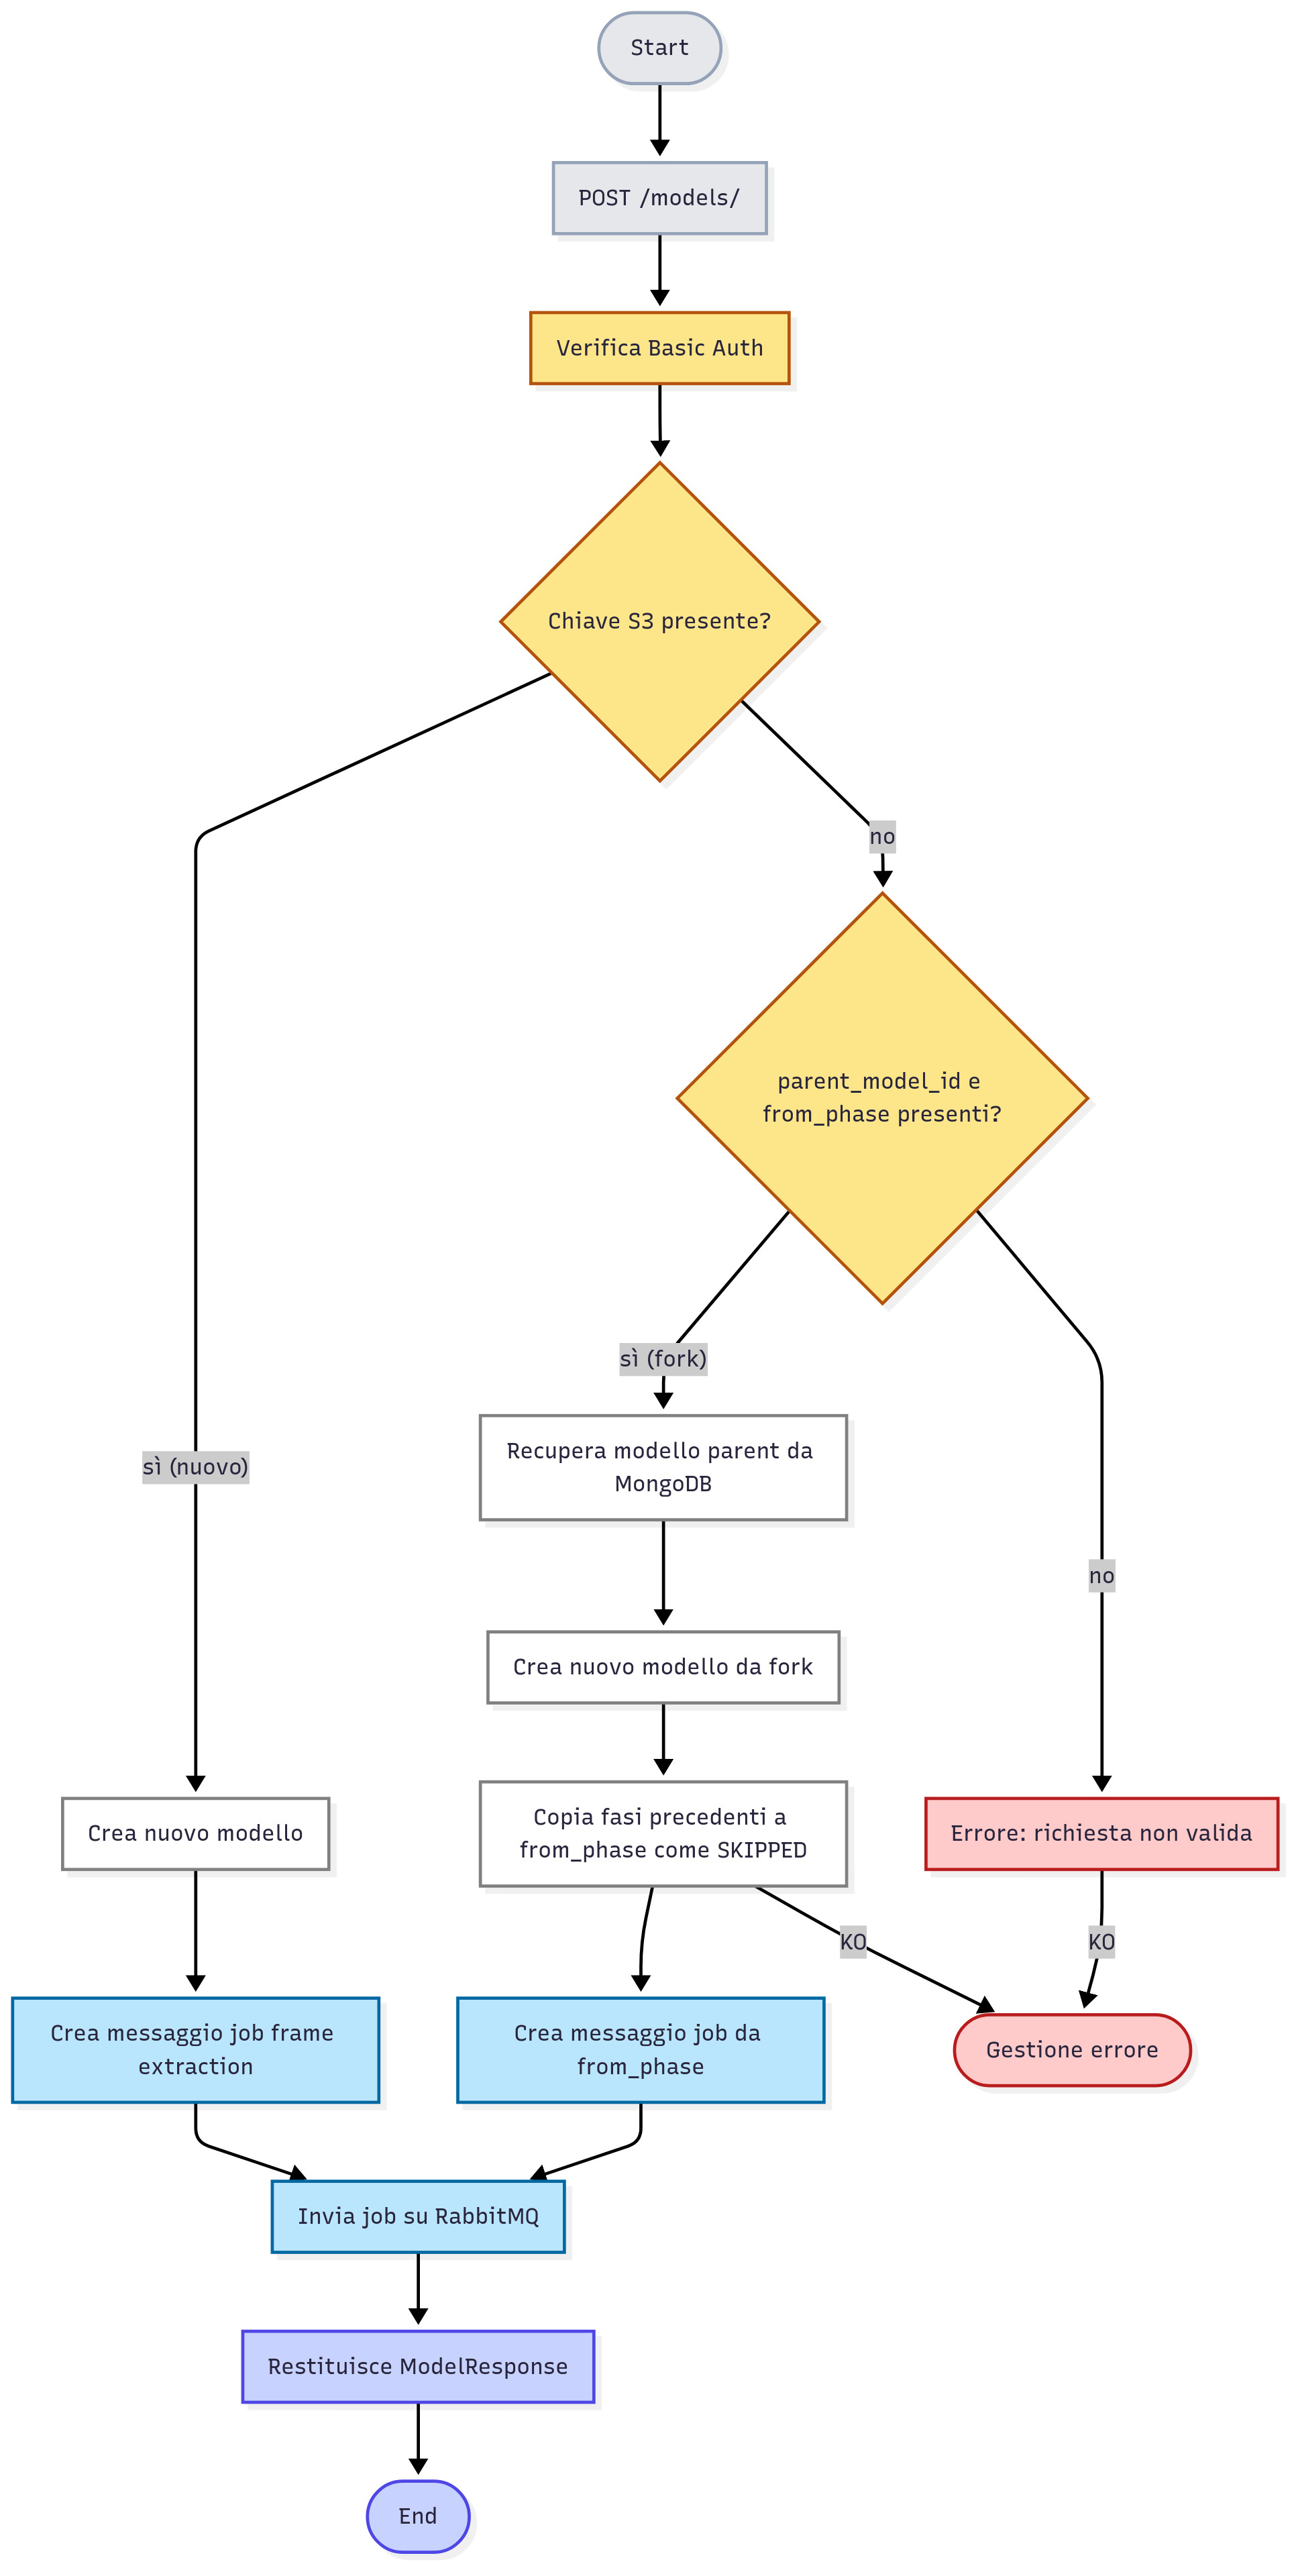
\includegraphics[width=0.5\textwidth]{images/create_or_fork_diagram.jpg}
	\caption{Diagramma per creazione e fork modello}
	\label{fig:create_or_fork_diagram}
\end{figure}

\begin{figure}[p]
	\centering
	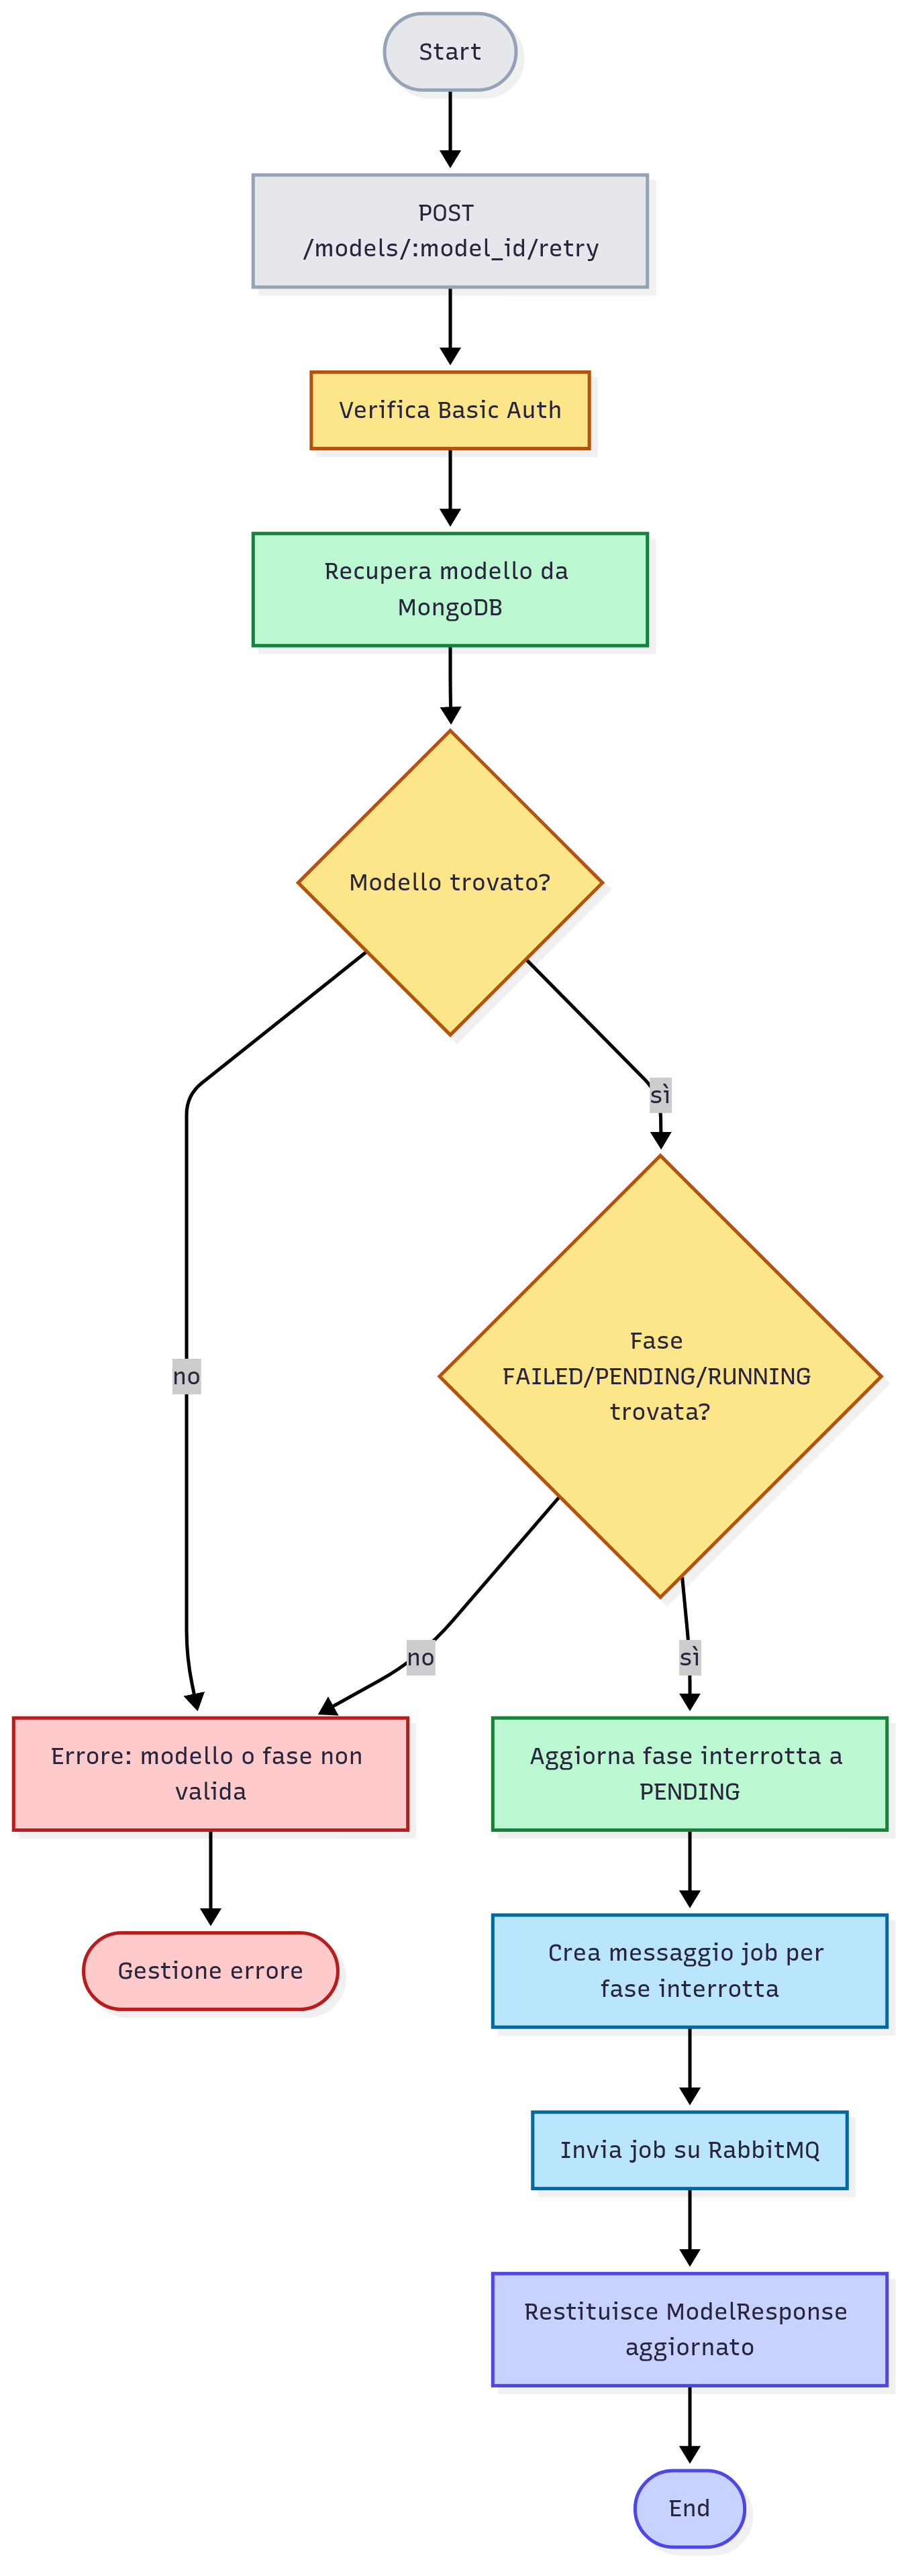
\includegraphics[width=0.5\textwidth]{images/retry_model_diagram.jpg}
	\caption{Diagramma per retry del modello}
	\label{fig:retry_diagram}
\end{figure}

\newpage
\subsection{Notifiche push in real-time}
Ogni volta che avviene un cambiamento rilevante nello stato dei modelli all’interno del database, il sistema è in grado di propagare in tempo reale una notifica ai client connessi. Dopo l’apertura della connessione WebSocket, il frontend riceve aggiornamenti direttamente dall’API Gateway, garantendo all’utente informazioni sempre aggiornate sull’avanzamento delle elaborazioni, senza la necessità di refresh manuali o polling periodico.

\begin{figure}[ht]
	\centering
	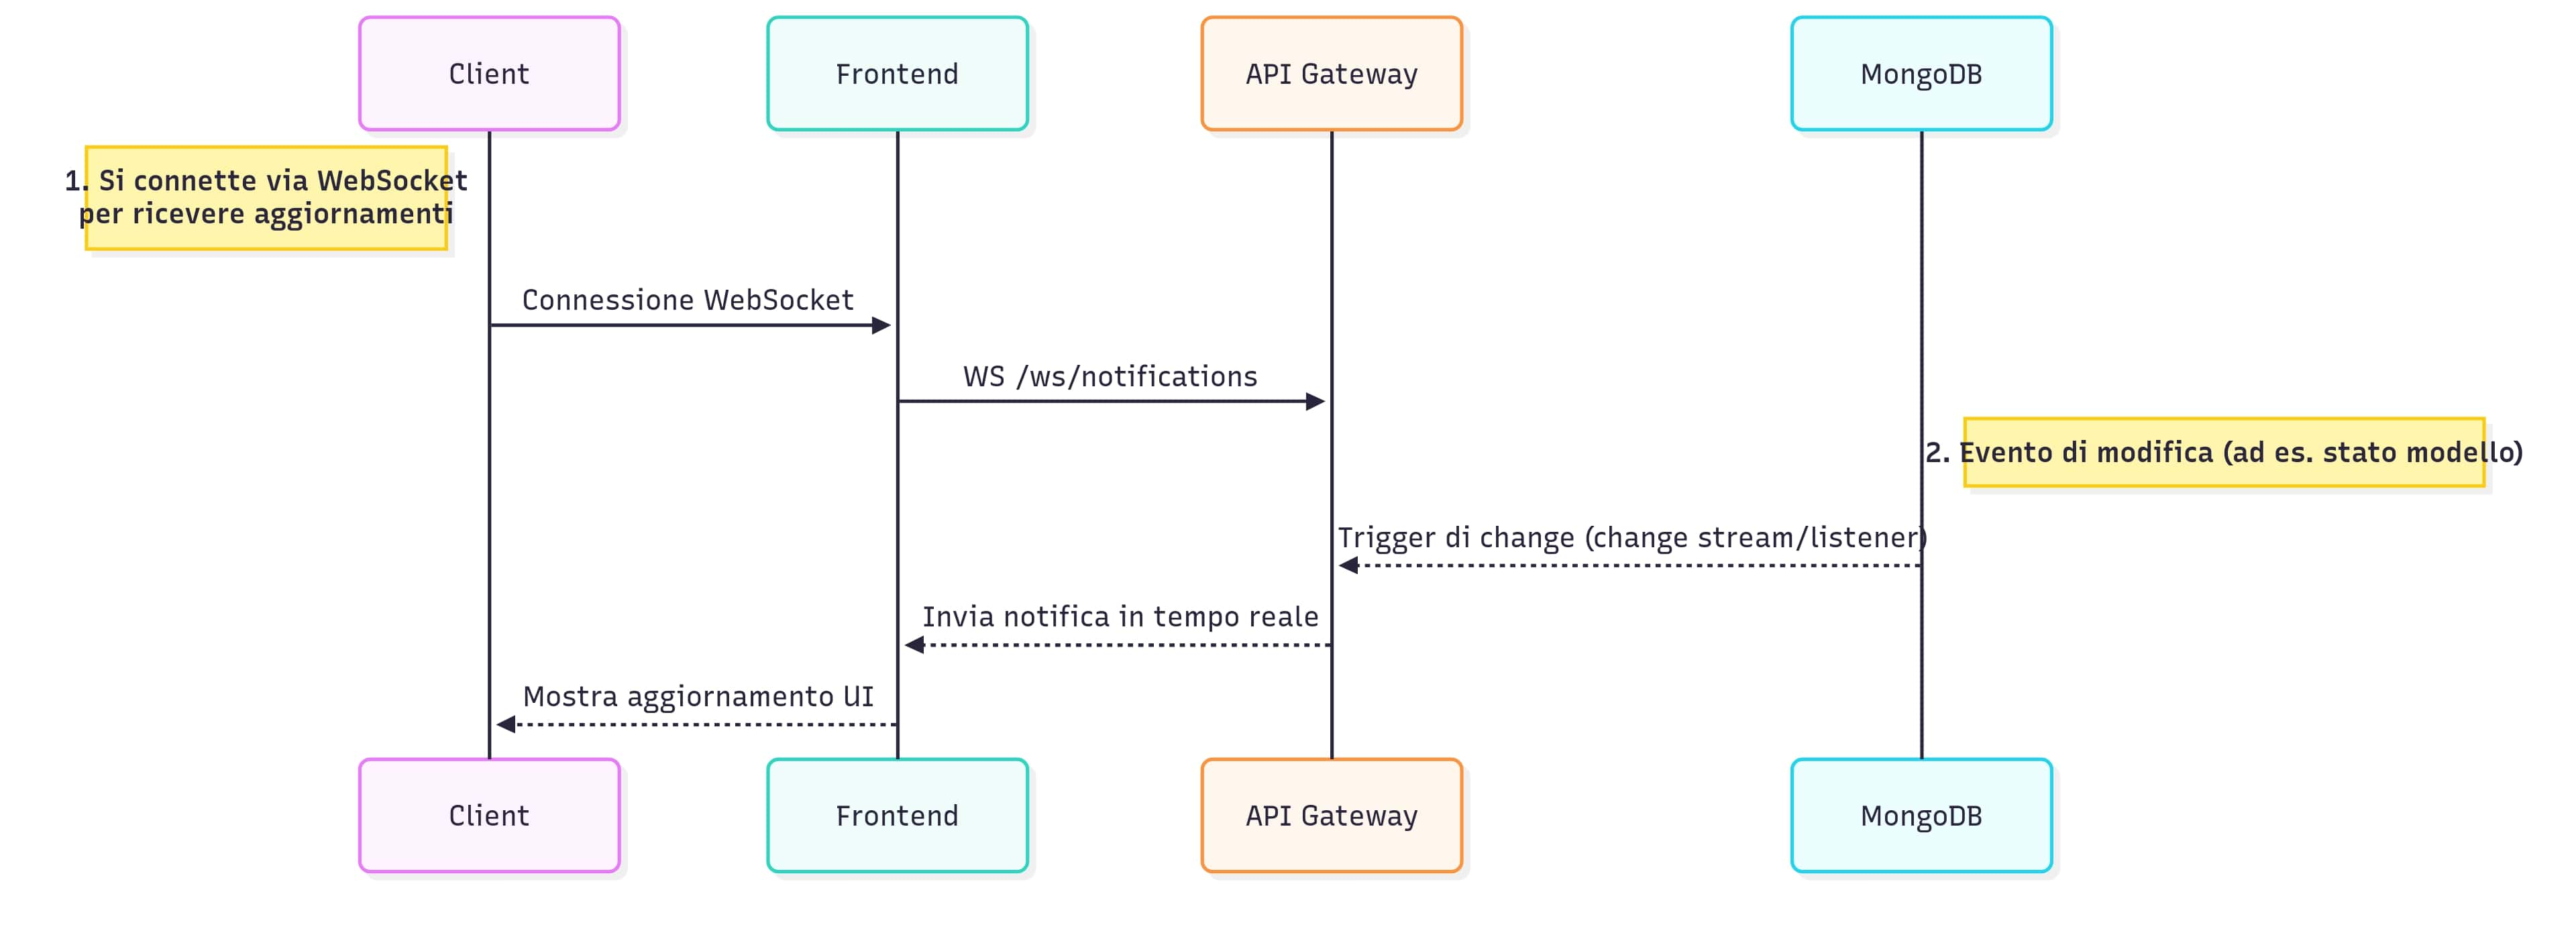
\includegraphics[width=0.9\textwidth]{images/push_notification_flow.jpg}
	\caption{Flusso per notifiche push in real-time}
	\label{fig:push_notification}
\end{figure}
\subsection{Considerazioni e Best Practice}

Il design di questo API Gateway consente di centralizzare la logica di business e la gestione della sicurezza, semplificando l’interazione tra frontend e servizi backend. La scelta di endpoint RESTful chiari, l’uso di WebSocket per le notifiche e l’integrazione di presigned URL per gli upload garantiscono \textbf{scalabilità, sicurezza e facilità d’integrazione}.


		


\section{Layer di Presentazione}

\subsection{Architettura dell'interfaccia utente}

Il frontend del sistema implementa un'interfaccia web moderna e responsiva progettata per rendere accessibile la tecnologia del 3D Gaussian Splatting a utenti non tecnici. L'applicazione, sviluppata con Vue.js 3 e Vuetify\footnote{https://vuetifyjs.com/en/}, offre un'esperienza utente coerente e intuitiva attraverso componenti Material Design ottimizzati per la gestione di workflow complessi.

\subsubsection{Dashboard Principale}

La dashboard rappresenta il punto di ingresso principale del sistema, organizzata secondo principi di information architecture che privilegiano la scansione rapida e l'accesso immediato alle funzionalità chiave. L'interfaccia adotta un layout a griglia responsivo che visualizza i modelli come card informative, ciascuna contenente:

\begin{itemize}
	\item \textbf{Preview thumbnail} del modello renderizzato, generata automaticamente alla conclusione della prima fase del workflow (estrazione dei frame).
	\item \textbf{Badge informativi} che comunicano immediatamente engine utilizzato (INRIA, MCMC, TAMING) e livello di qualità (Fast, Balanced, Quality)
	\item \textbf{Status indicator} con codifica cromatica per identificare rapidamente lo stato di elaborazione
	\item \textbf{Timeline di processing} che visualizza le cinque fasi del workflow con tempi di esecuzione individuali
	\item \textbf{Metriche di qualità} (PSNR, SSIM, LPIPS) presentate in formato espandibile per non sovraccaricare l'interfaccia
\end{itemize}

\begin{figure}[htbp]
	\centering
	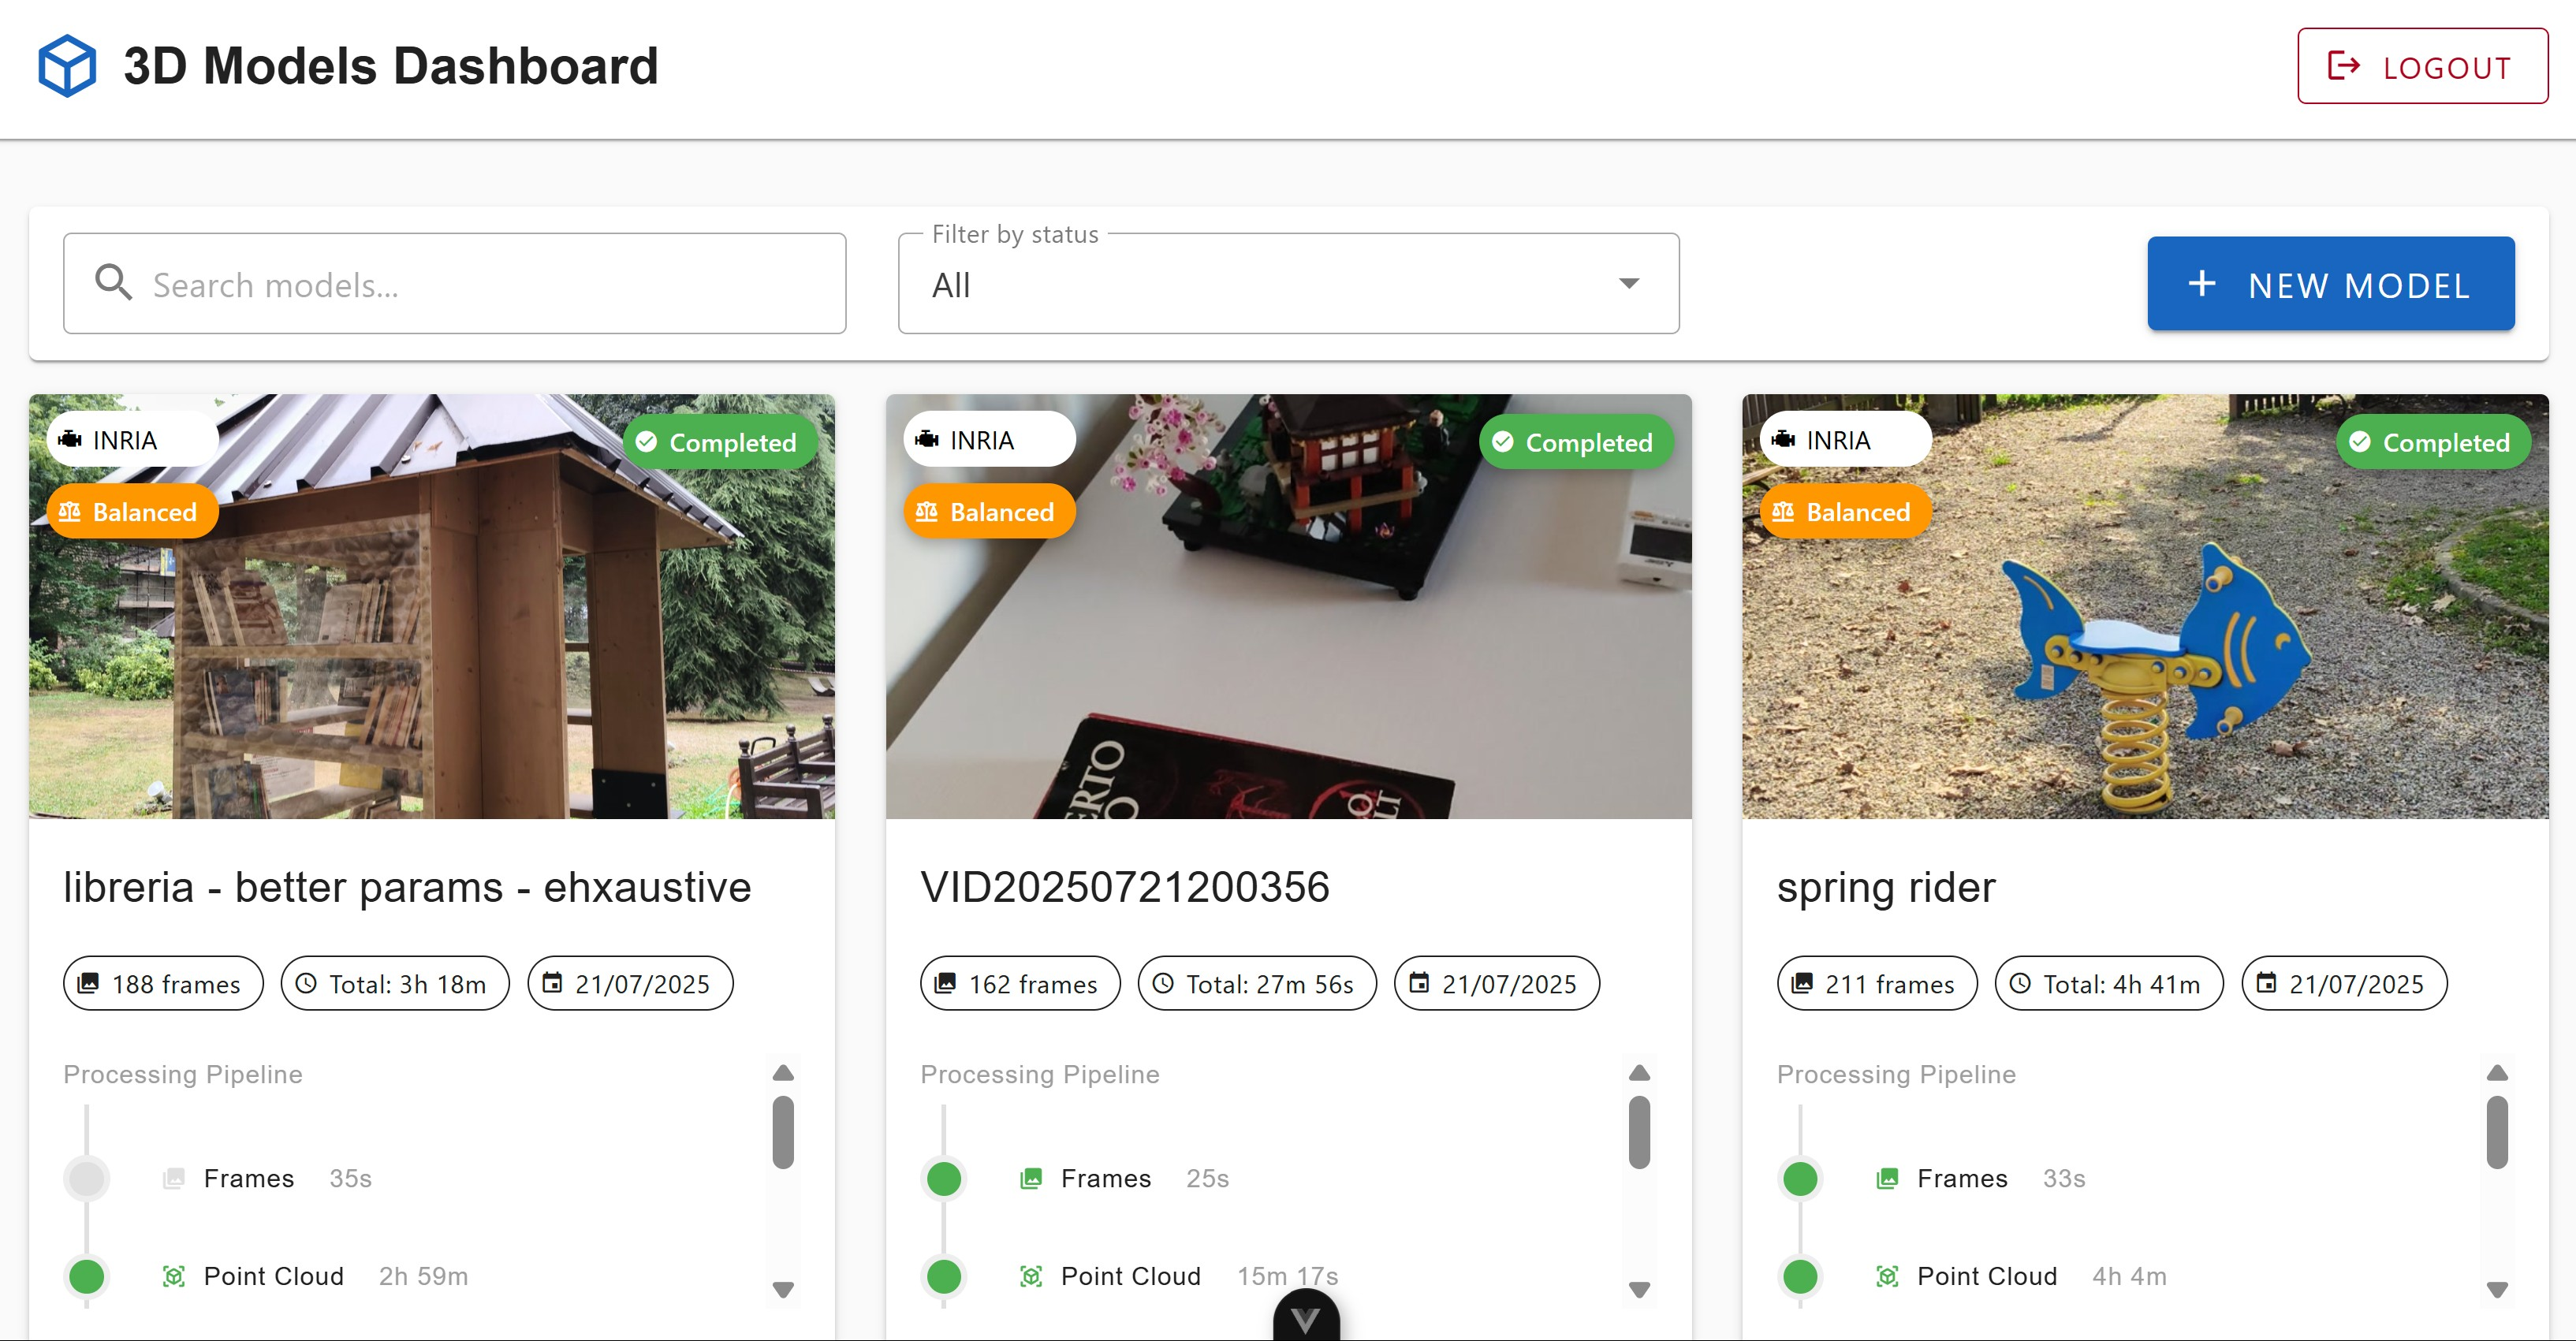
\includegraphics[width=\textwidth]{images/fronted_list.jpg}
	\caption{Dashboard principale con vista a griglia dei modelli, filtri di ricerca e indicatori di stato}
	\label{fig:dashboard_main}
\end{figure}

Il sistema di \textbf{filtraggio e ricerca} permette agli utenti di navigare efficacemente anche in presenza di centinaia di modelli, con filtri per stato, ricerca testuale e paginazione server-side che garantisce performance costanti indipendentemente dal volume di dati.

\subsubsection{Gestione del Workflow Utente}

L'interfaccia implementa tre modalità principali di creazione modelli, ciascuna ottimizzata per specifici scenari d'uso:

\paragraph{Creazione di un nuovo modello}
Il dialog di creazione nuovo modello guida l'utente attraverso un processo step-by-step che include:
\begin{itemize}
	\item Upload diretto del video tramite drag-and-drop o selezione file
	\item Configurazione intuitiva dei parametri attraverso slider visuali e card informative
	\item Preview real-time della pipeline di elaborazione che verrà eseguita
	\item Sistema di rating visuale per comunicare l'impatto delle scelte su velocità, qualità e requisiti hardware
\end{itemize}

\begin{figure}[htbp]
	\centering
	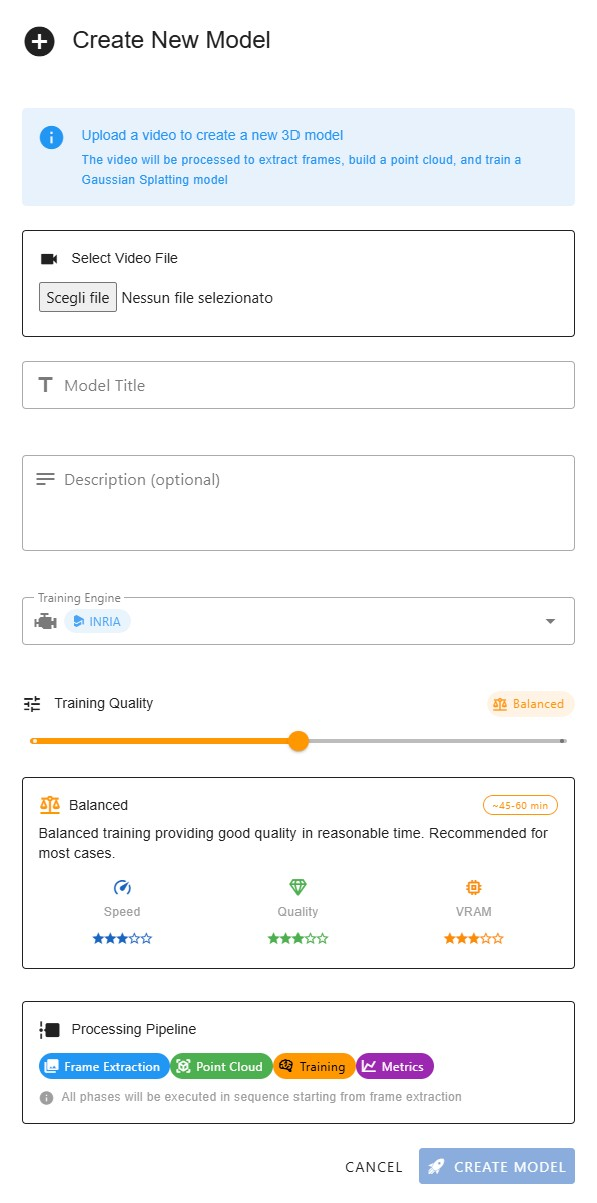
\includegraphics[width=0.7\textwidth]{images/fronted_new.jpg}
	\caption{Dialog di creazione nuovo modello con selezione engine e configurazione qualità tramite slider interattivo}
	\label{fig:new_model_dialog}
\end{figure}

\paragraph{Fork di un modello preesistente}
La funzionalità di fork permette di creare varianti di modelli esistenti riutilizzando fasi già completate. L'interfaccia visualizza chiaramente:
\begin{itemize}
	\item Quali fasi verranno riutilizzate (indicate con icona di cache)
	\item Da quale punto ripartirà l'elaborazione
	\item Stima del risparmio temporale rispetto a una nuova elaborazione completa
\end{itemize}

\begin{figure}[htbp]
	\centering
	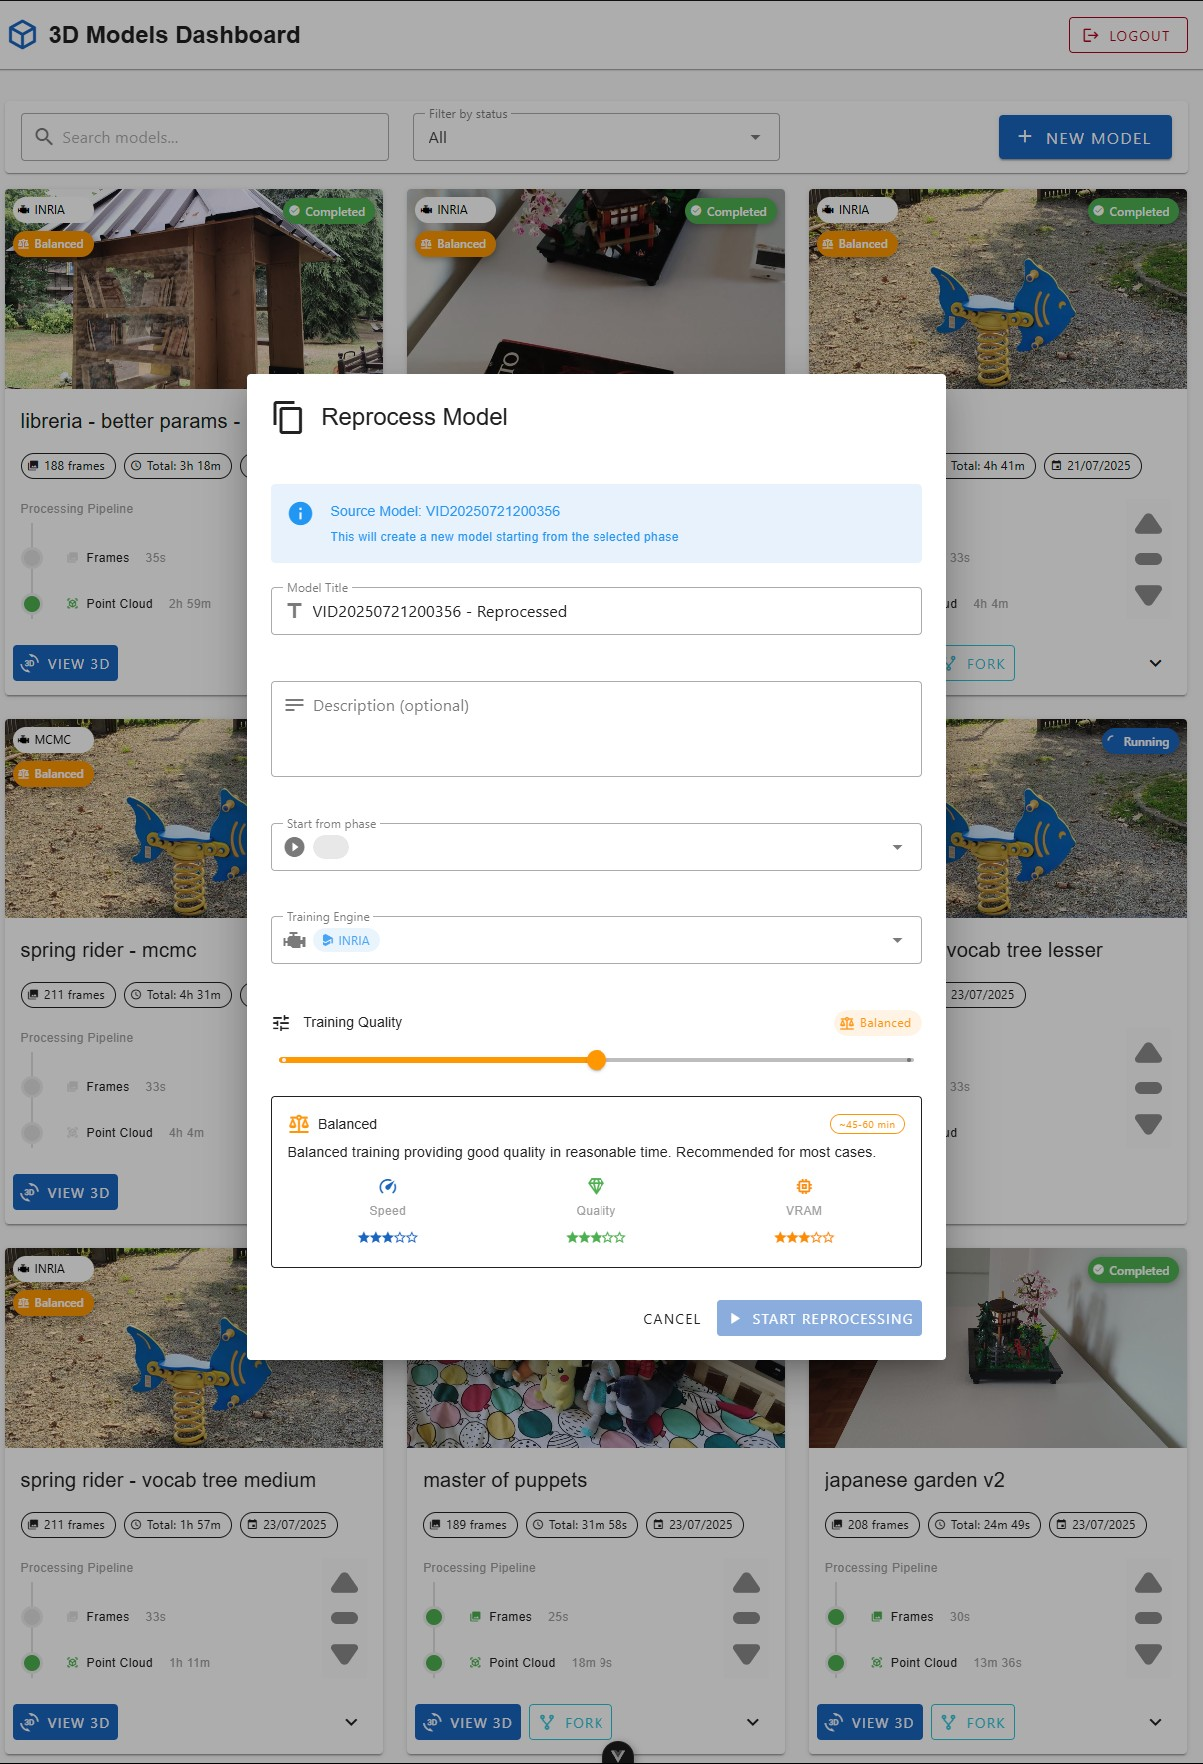
\includegraphics[width=0.8\textwidth]{images/frontend_fork.jpg}
	\caption{Dialog di reprocessing che mostra la selezione della fase di partenza e le fasi che verranno riutilizzate}
	\label{fig:fork_dialog}
\end{figure}

\paragraph{Retry intelligente}
Per modelli con elaborazione fallita, il sistema identifica automaticamente l'ultima fase completata con successo e propone di riprendere da quel punto, preservando il lavoro computazionale già svolto.

\subsection{Sistema di notifiche real-time}

Il frontend implementa un sofisticato sistema di notifiche basato su WebSocket che mantiene gli utenti informati sull'avanzamento delle elaborazioni senza richiedere refresh manuali della pagina.

\subsubsection{Architettura delle Notifiche}

Il sistema utilizza un approccio multi-livello per la gestione delle notifiche composto da:

\begin{itemize}
\item Toast Notifications: messaggi temporanei non invasivi che appaiono nell'angolo superiore destro per eventi chiave come completamento fasi o cambiamenti di stato. Ogni notifica è contestualizzata con icone e colori appropriati al tipo di evento.

\item  Notification Drawer:
un pannello laterale accessibile tramite FAB (Floating Action Button) che mantiene uno storico delle notifiche recenti. Il drawer implementa:
\begin{itemize}
	\item Raggruppamento intelligente per modello
	\item Indicatori di lettura/non lettura
	\item Timestamp relativi ("2 ore fa") per immediata comprensione temporale
	\item Azioni rapide per navigare al modello correlato
\end{itemize}

\begin{figure}[htbp]
	\centering
	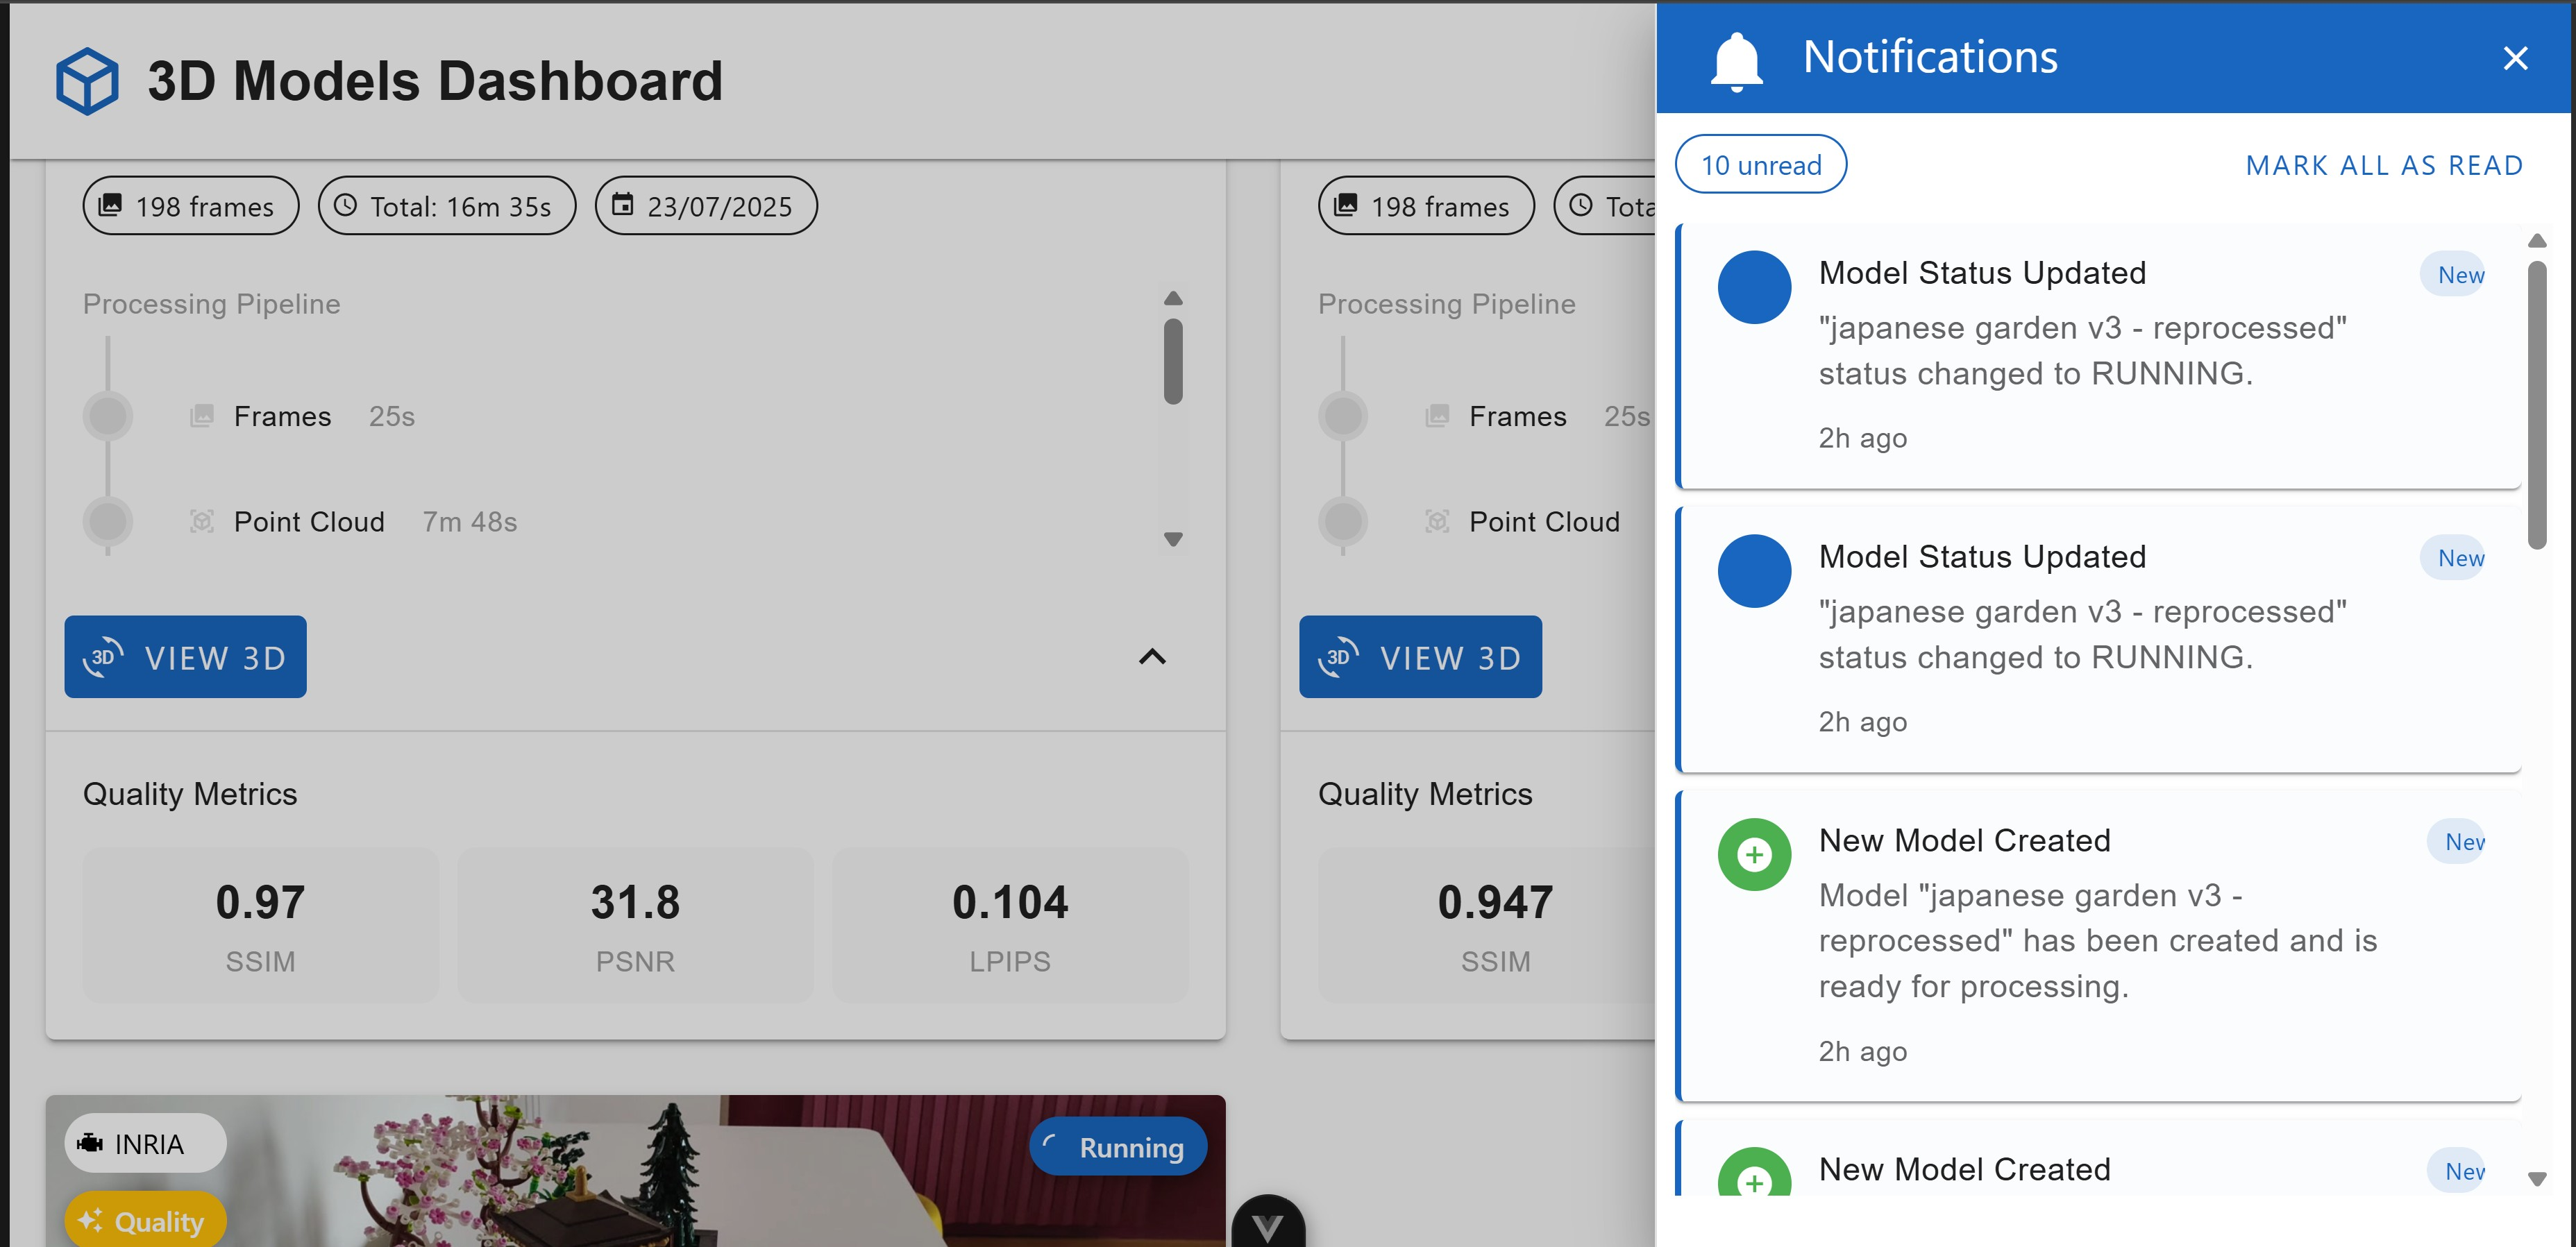
\includegraphics[width=0.9\textwidth]{images/frontend_notifications.jpg}
	\caption{Sistema di notifiche con drawer laterale che mostra lo storico degli eventi e badge per notifiche non lette}
	\label{fig:notification_drawer}
\end{figure}

\item Live Updates
La dashboard si aggiorna automaticamente quando arrivano notifiche relative a modelli visibili nella pagina corrente, eliminando la necessità di polling manuale e garantendo che le informazioni visualizzate siano sempre aggiornate.
\end{itemize}
\subsubsection{Gestione stati di connessione}
Il sistema monitora costantemente lo stato della connessione WebSocket, fornendo feedback visuale quando la connessione viene persa e implementando meccanismi di riconnessione automatica con backoff esponenziale per gestire interruzioni temporanee di rete.

\begin{figure}[htbp]
	\centering
	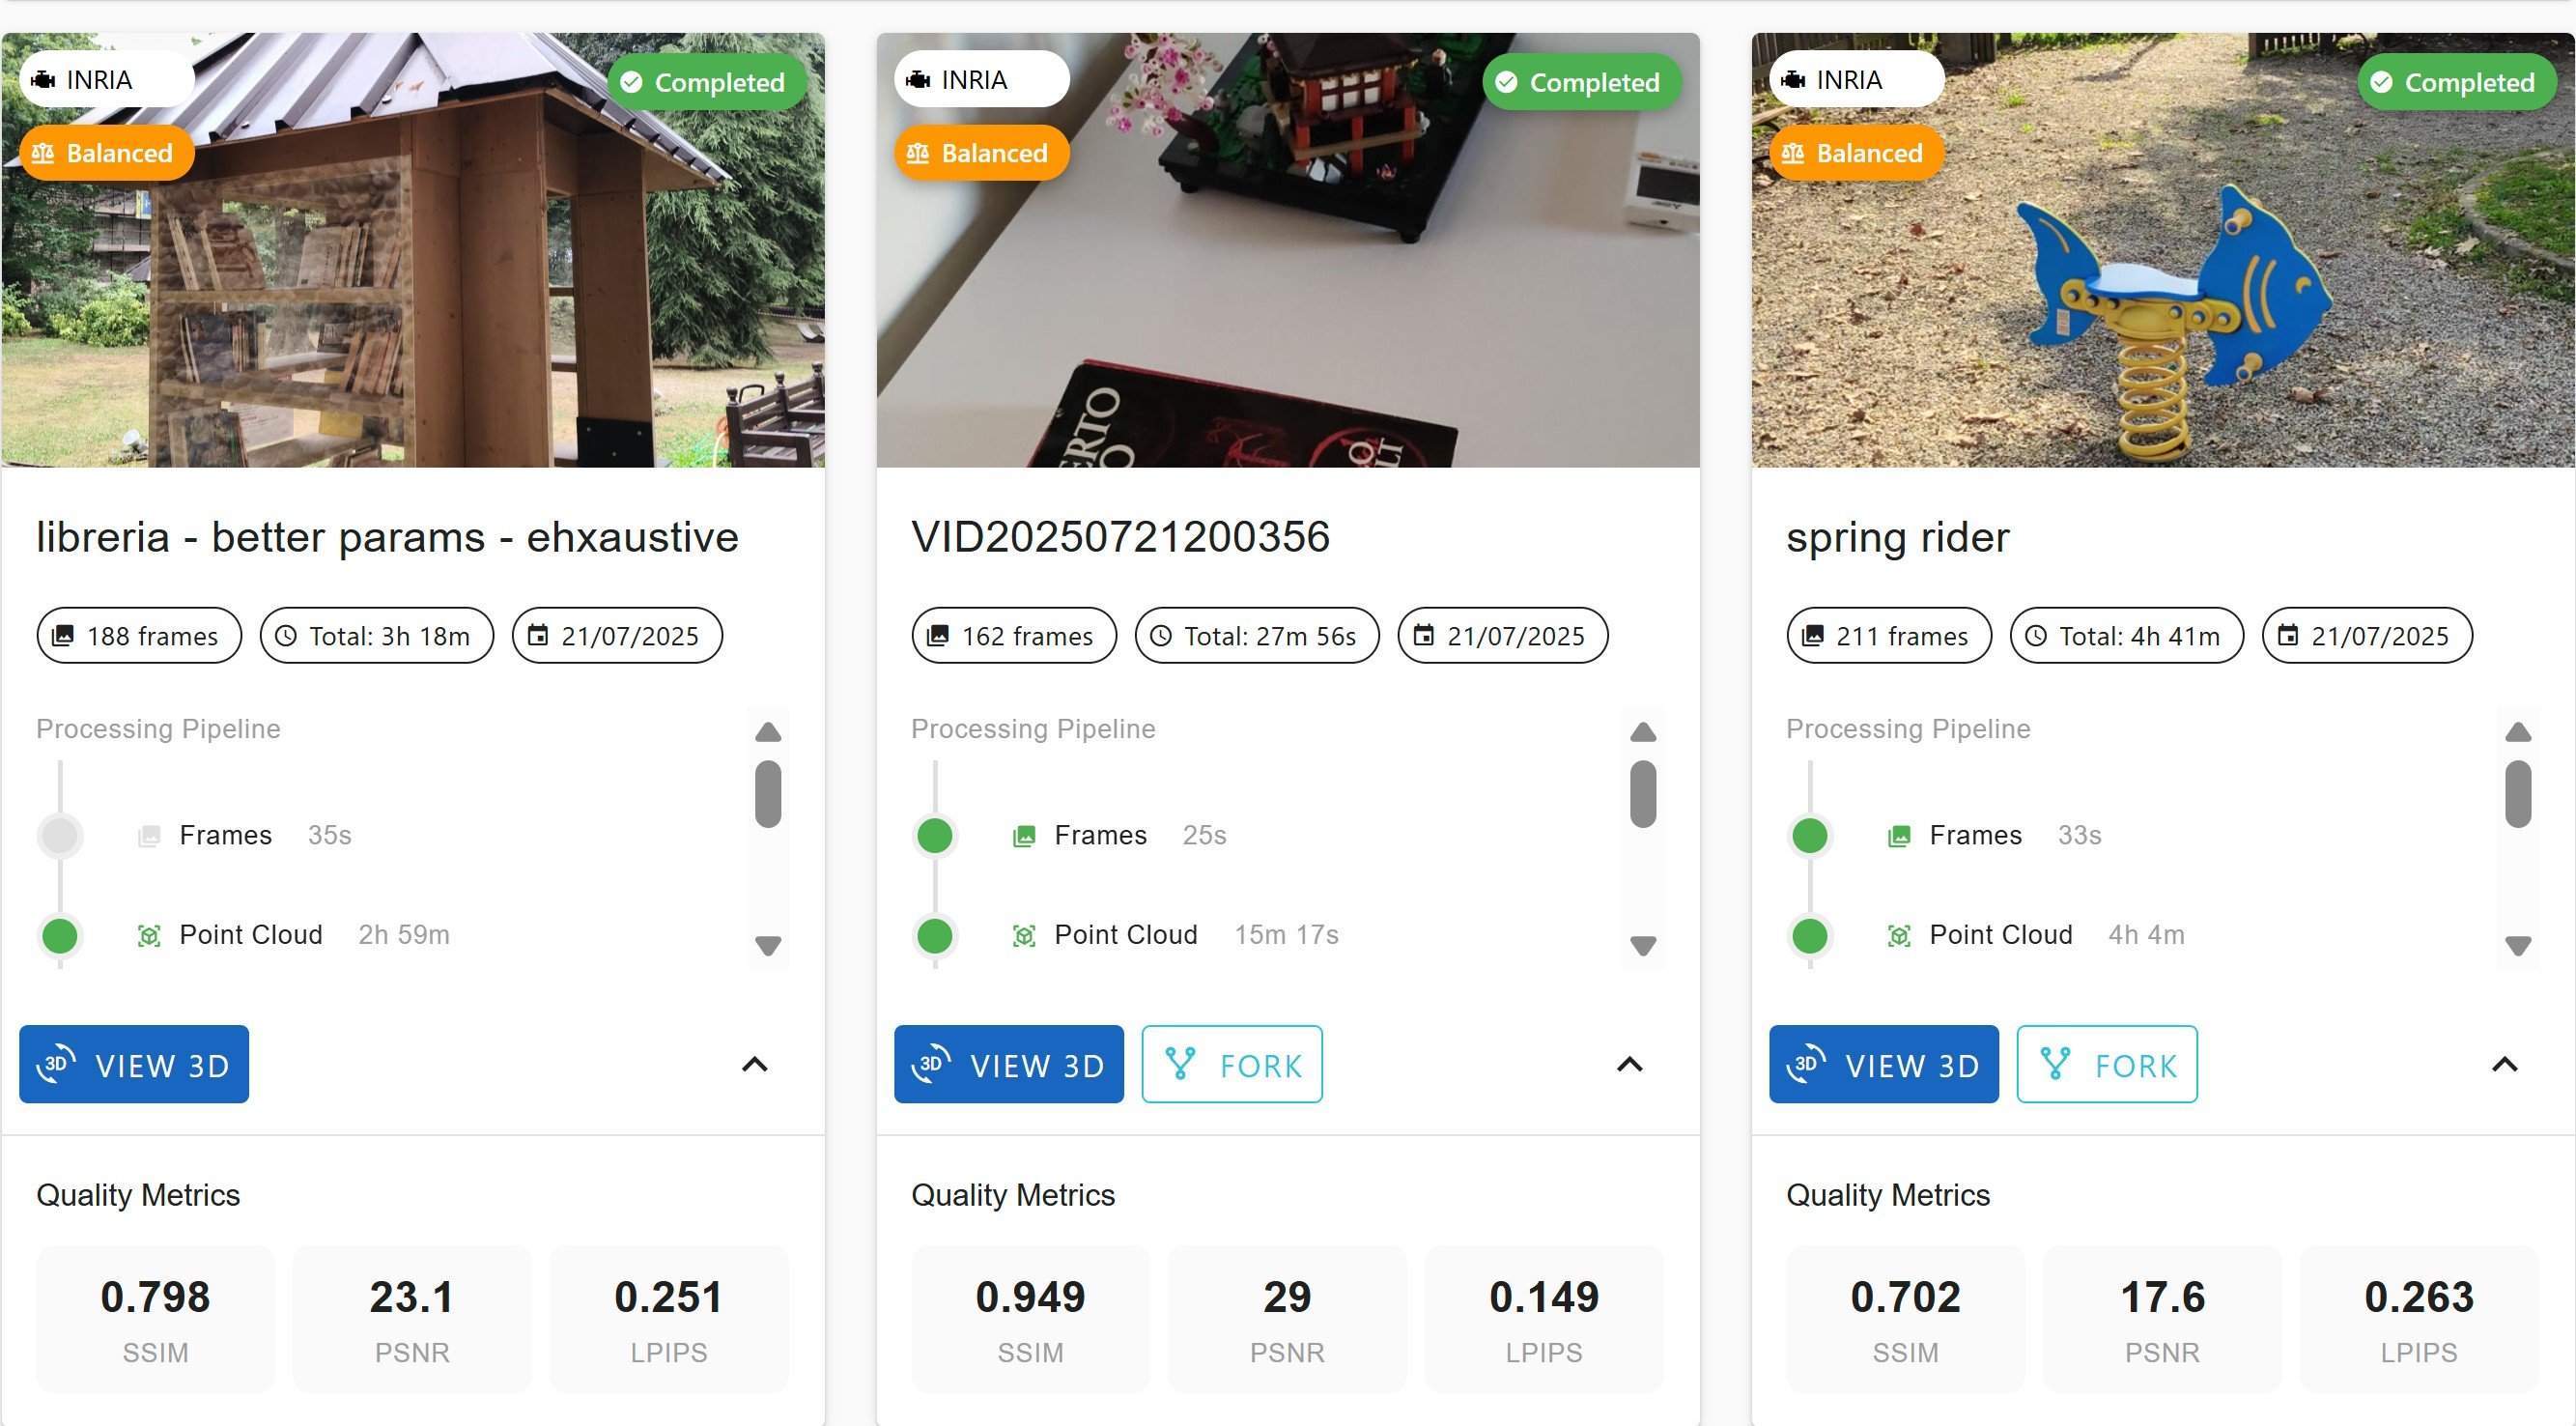
\includegraphics[width=\textwidth]{images/frontend_show_metrics.jpg}
	\caption{Vista espansa delle metriche di qualità (SSIM, PSNR, LPIPS) per confronto rapido tra modelli}
	\label{fig:dashboard_metrics}
\end{figure}

\subsection{Visualizzatore 3D Integrato}

Il componente di visualizzazione 3D rappresenta il culmine dell'esperienza utente, permettendo l'esplorazione interattiva dei modelli generati direttamente nel browser.

\subsubsection{Tecnologia di Rendering}

Il viewer utilizza la libreria \textbf{GaussianSplats3D} basata su Three.js, specificamente ottimizzata per il rendering efficiente di primitive gaussiane. Questa scelta tecnologica garantisce:

\begin{itemize}
	\item \textbf{Performance real-time}: Rendering a 60 FPS anche per modelli con centinaia di migliaia di splat
	\item \textbf{Compatibilità cross-platform}: Funzionamento su qualsiasi dispositivo con supporto WebGL
	\item \textbf{Interattività fluida}: Controlli camera intuitivi per rotazione, zoom e pan
\end{itemize}

\subsubsection{Interfaccia del Viewer}

Il viewer 3D implementa un'interfaccia minimalista che massimizza l'area di visualizzazione mantenendo accessibili le informazioni essenziali:

\paragraph{Overlay Informativo}
Un pannello semi-trasparente nell'angolo superiore sinistro visualizza:
\begin{itemize}
	\item Statistiche di rendering (FPS, numero di splat)
	\item Metriche di qualità del modello
	\item Engine e parametri utilizzati per il training
\end{itemize}

\begin{figure}[htbp]
	\centering
	\begin{subfigure}[b]{0.49\textwidth}
		\centering
		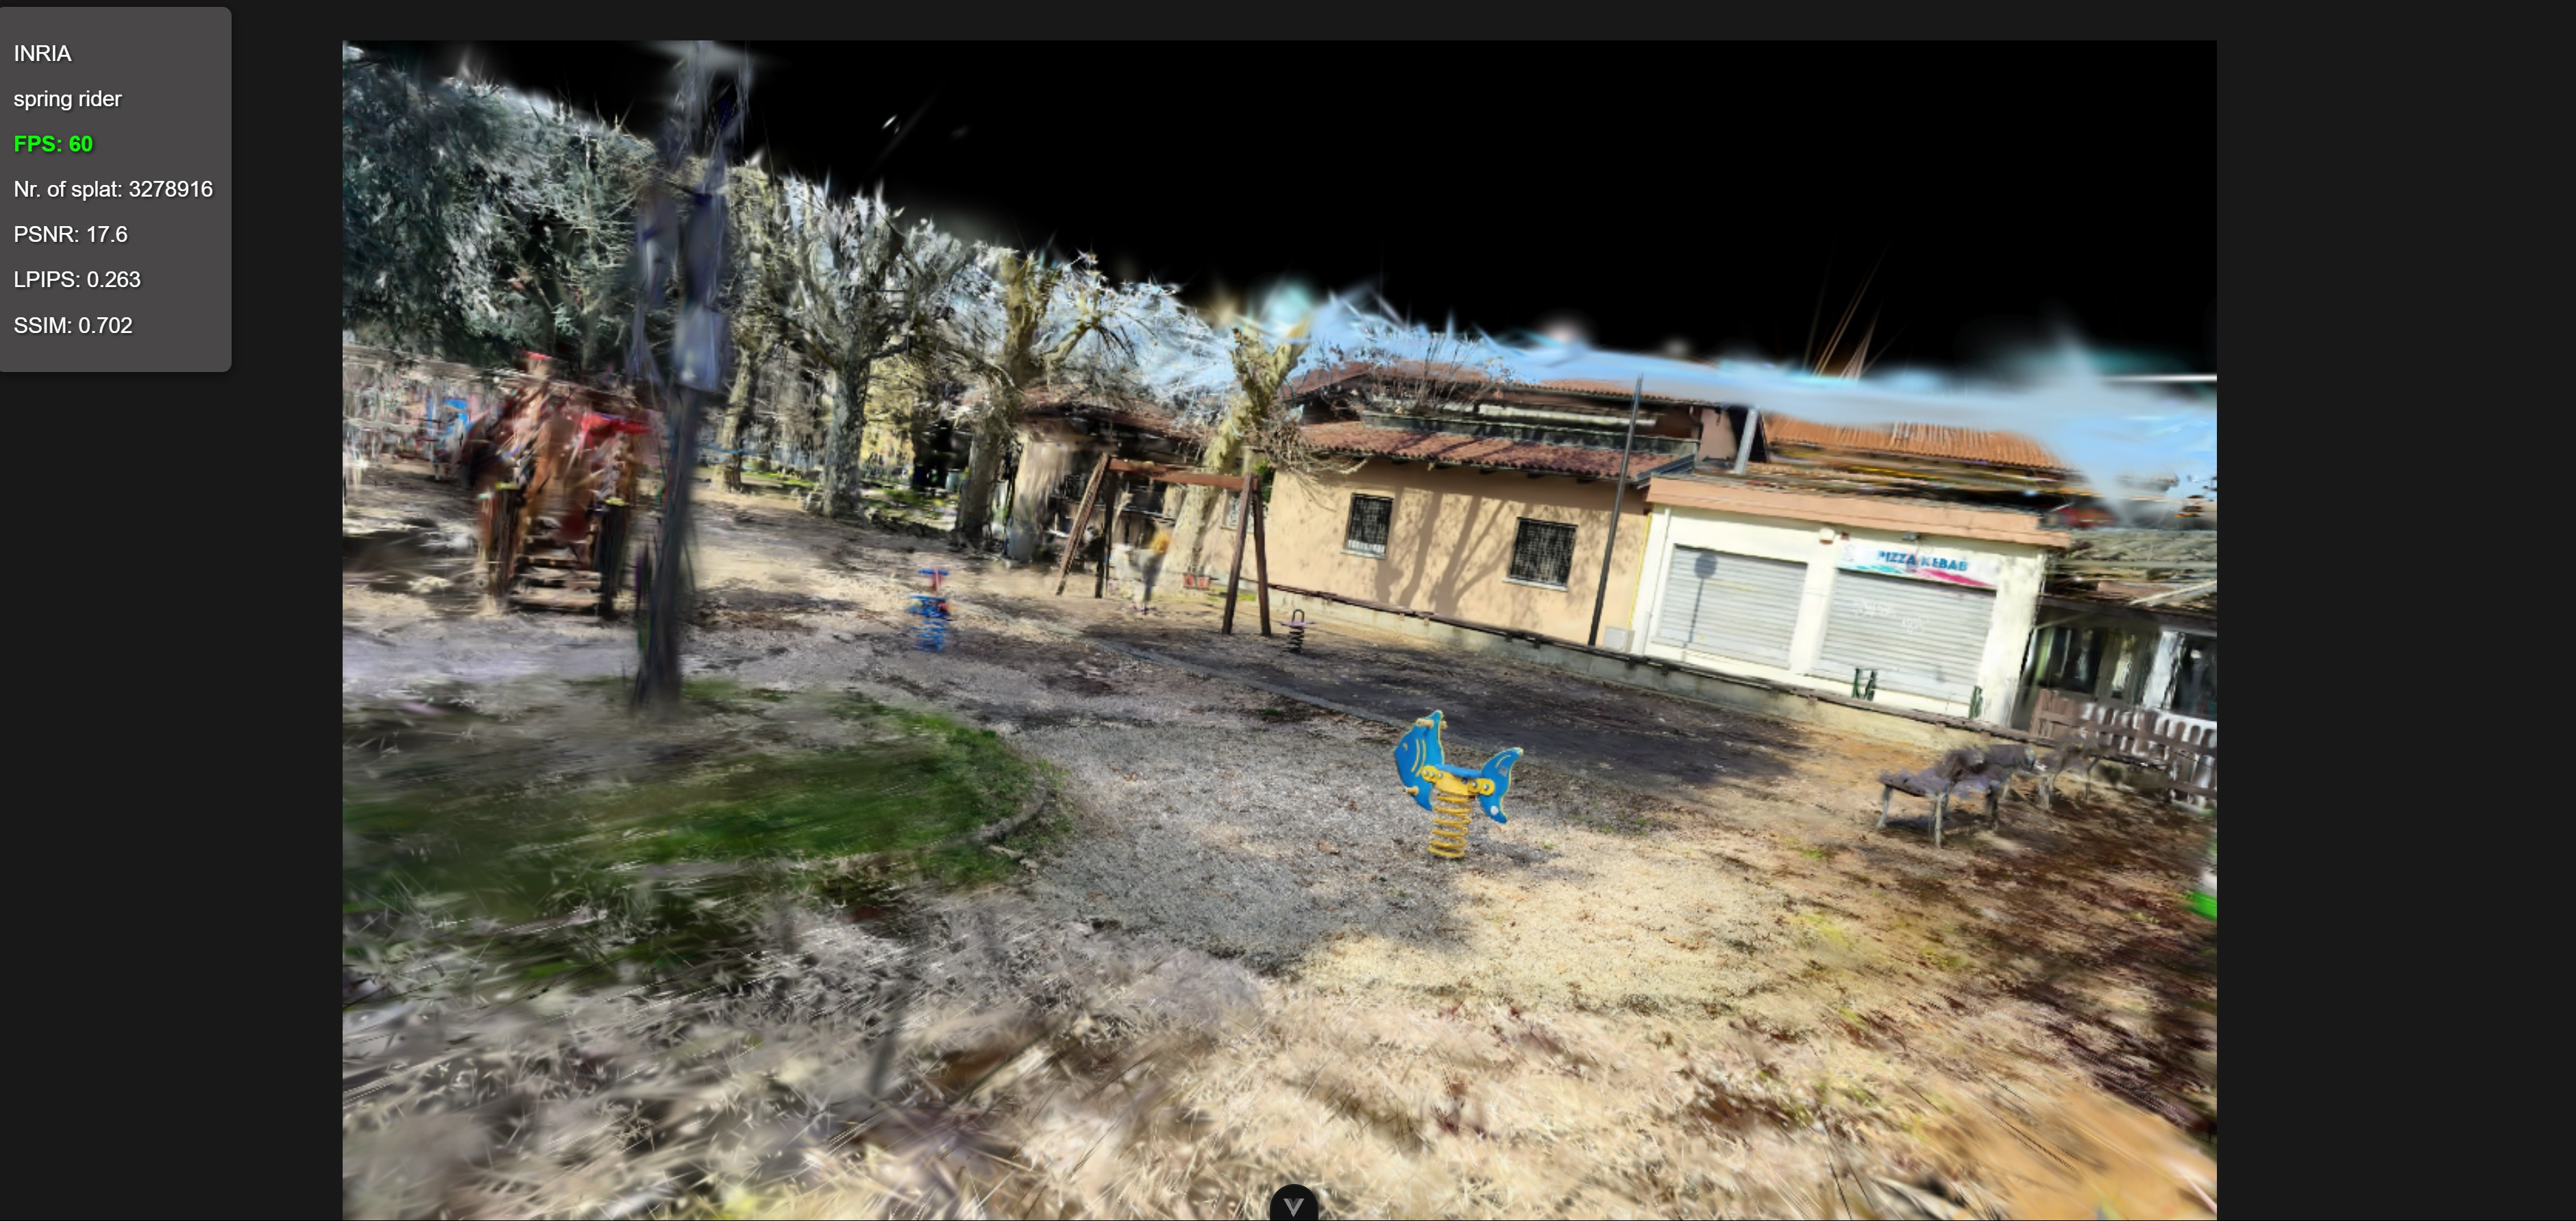
\includegraphics[width=\textwidth]{images/frontend_viewer.jpg}
		\caption{Spring rider - 327k splats}
	\end{subfigure}
	\hfill
	\begin{subfigure}[b]{0.49\textwidth}
		\centering
		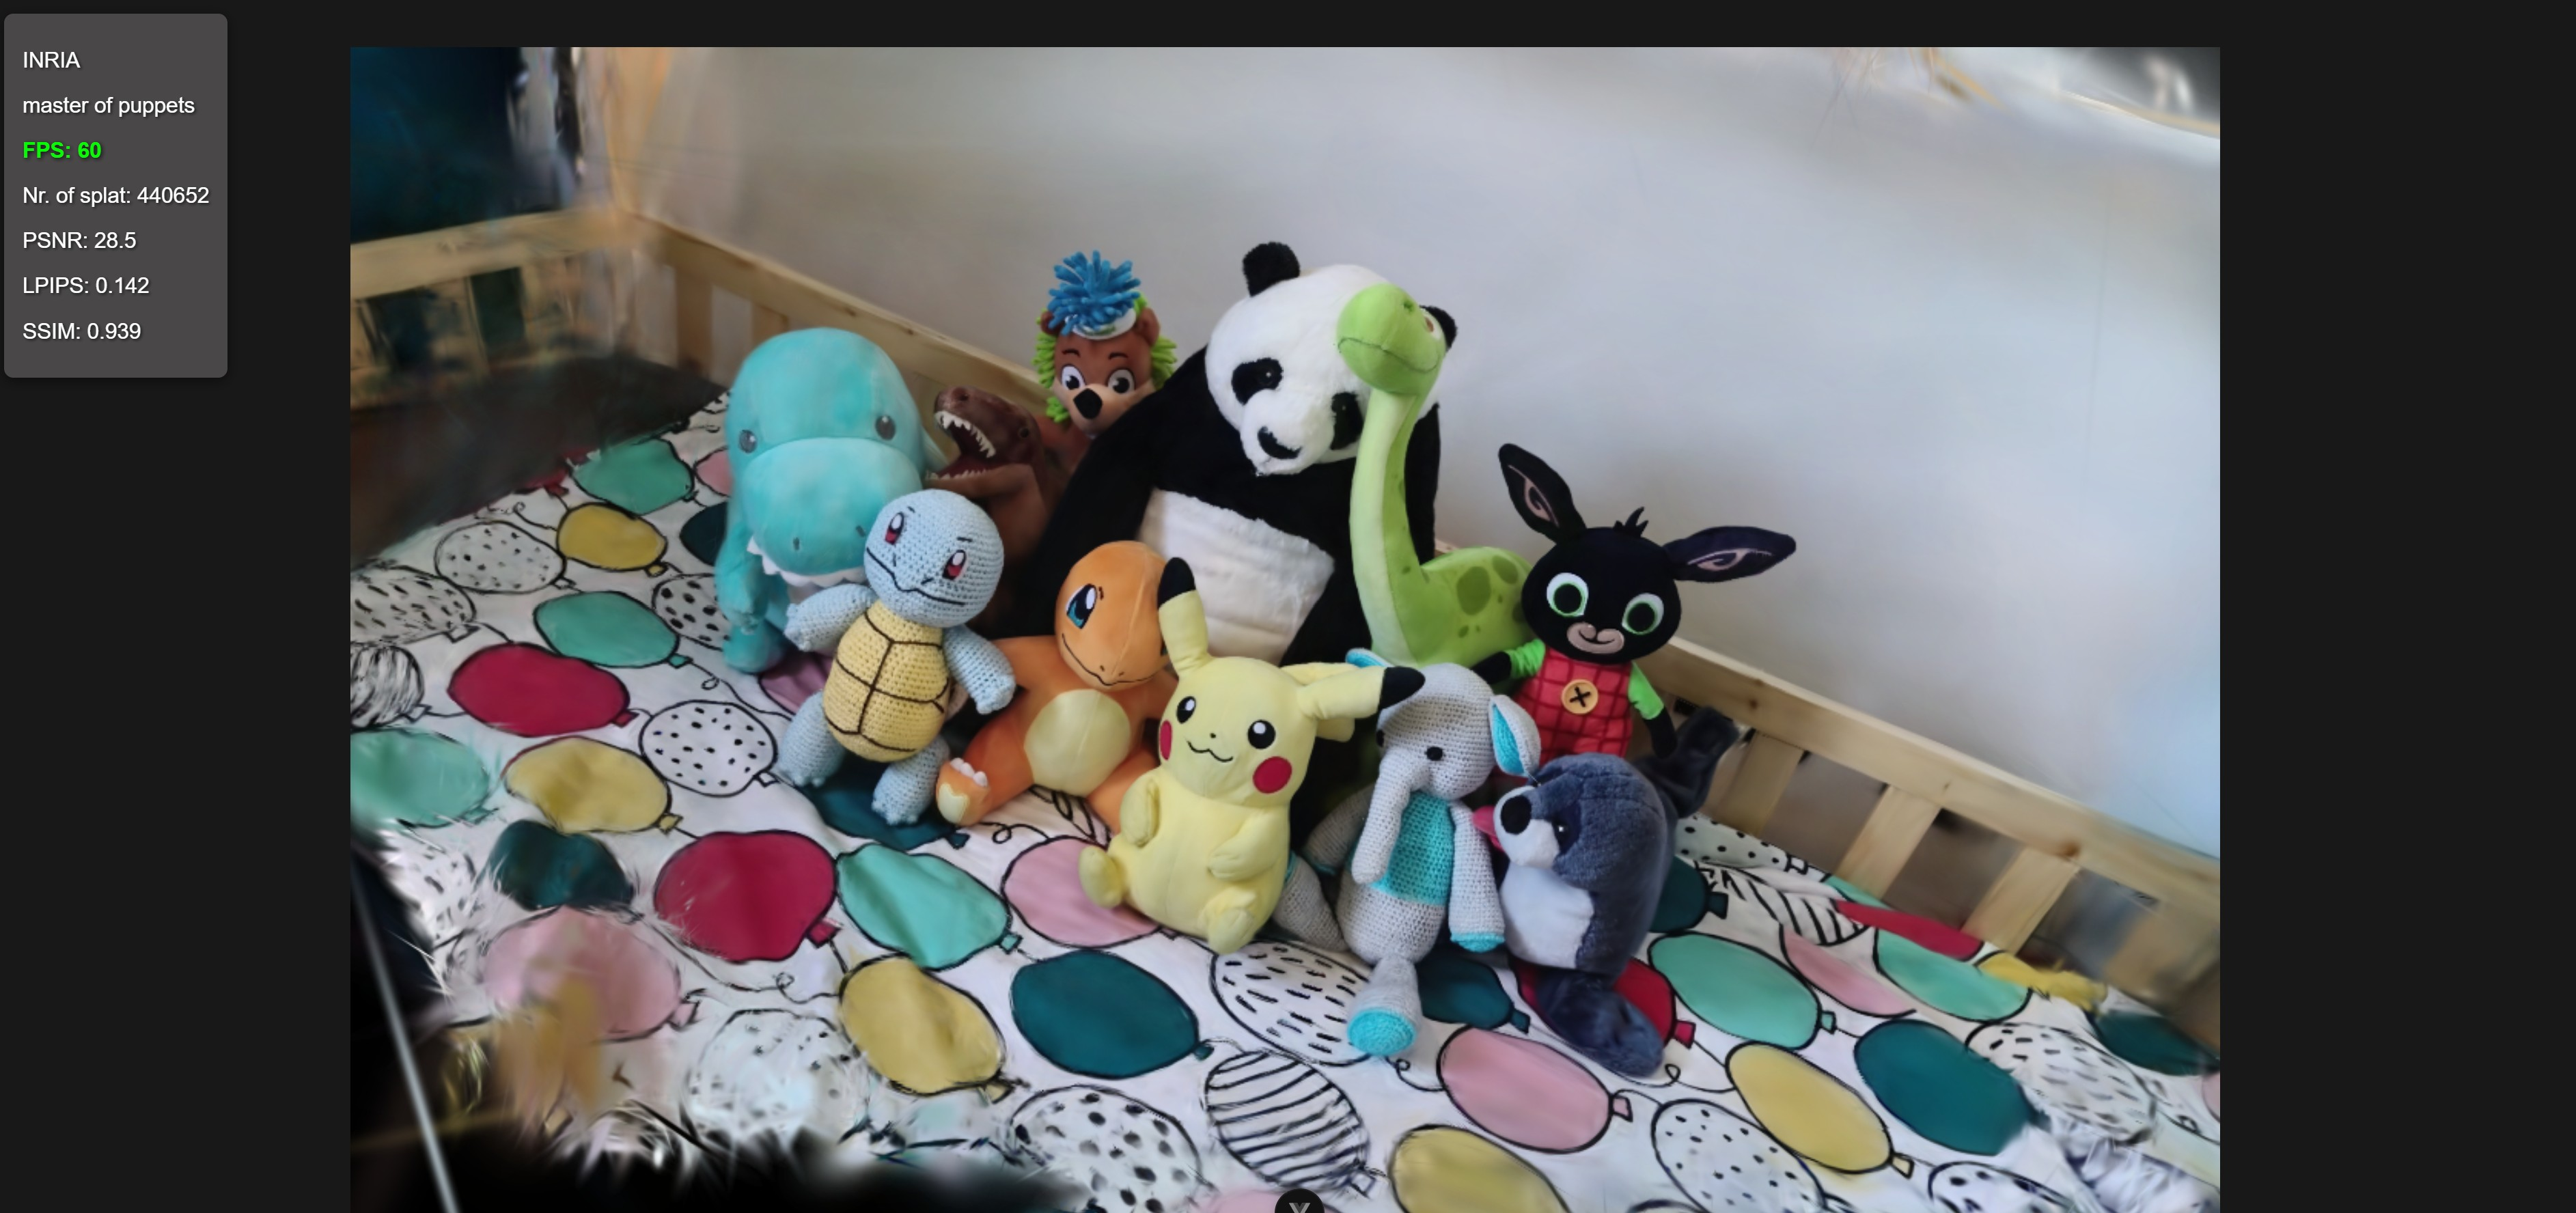
\includegraphics[width=\textwidth]{images/frontend_viewer_2.jpg}
		\caption{Master of puppets - 440k splats}
	\end{subfigure}
	\caption{Visualizzatore 3D integrato con overlay informativo mostrante FPS, numero di splat e metriche di qualità}
	\label{fig:viewer3d_examples}
\end{figure}

\paragraph{Controlli Camera}
Il sistema recupera automaticamente la posizione camera ottimale dal dataset di training, garantendo che il modello sia presentato dalla prospettiva più favorevole al primo caricamento. Gli utenti possono poi esplorare liberamente utilizzando controlli standard di navigazione 3D.

\paragraph{Gestione formati}
Il viewer gestisce trasparentemente la conversione tra formati, accettando sia file PLY che SPLAT ottimizzati e applicando le trasformazioni necessarie per la corretta visualizzazione, incluse conversioni di opacità specifiche per diversi algoritmi di training.

\begin{figure}[htbp]
	\centering
	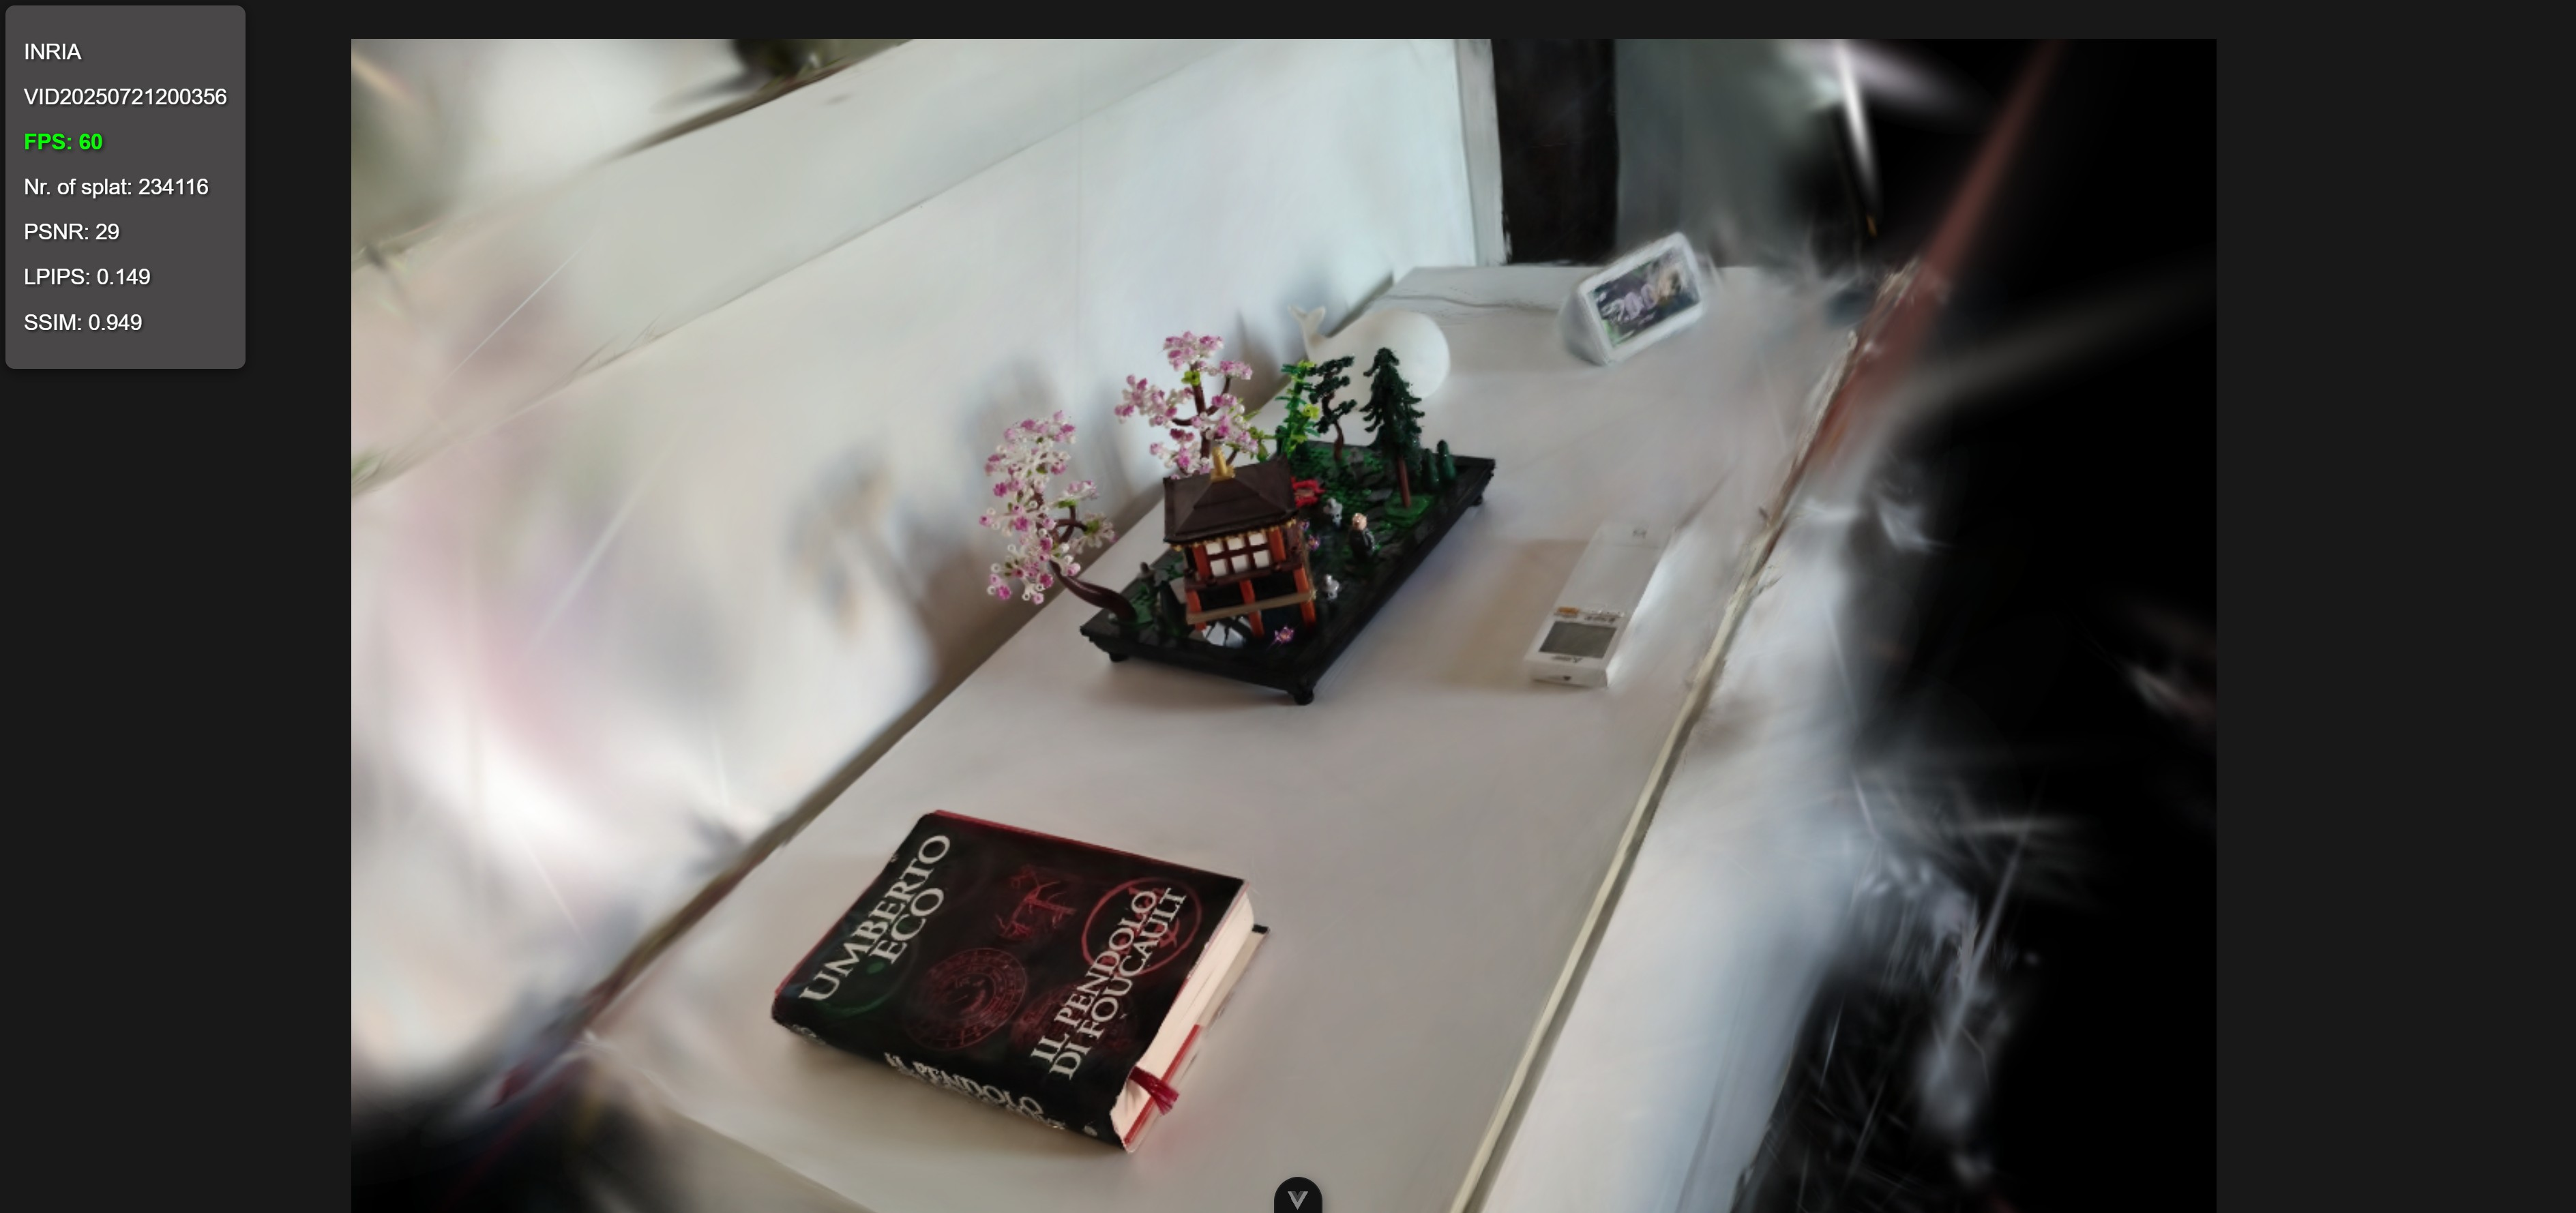
\includegraphics[width=\textwidth]{images/frontend_viewer_3.jpg}
	\caption{Visualizzazione di un modello complesso (Japanese garden) con rendering real-time a 60 FPS}
	\label{fig:viewer3d_complex}
\end{figure}
\newpage
\subsection{Ottimizzazione performance e UX}

Il frontend implementa diverse strategie per garantire un'esperienza utente fluida anche con dataset di grandi dimensioni:

\paragraph{Lazy Loading}
Le thumbnail e i dati dei modelli vengono caricati progressivamente durante lo scroll, riducendo il tempo di caricamento iniziale della dashboard.

\paragraph{Caching intelligente}
I modelli 3D visualizzati recentemente vengono mantenuti in cache del browser, permettendo switching istantaneo tra modelli già caricati.

\paragraph{Responsive Design}
Layout adattivi garantiscono usabilità ottimale su dispositivi desktop, tablet e mobile, con breakpoint specificamente ottimizzati per i pattern di utilizzo tipici del sistema.

\subsection{Integrazione con il Backend}

Il frontend mantiene una separazione netta tra logica di presentazione e business logic attraverso l'utilizzo di \textbf{Pinia} per lo state management. Questo approccio centralizzato permette:

\begin{itemize}
	\item \textbf{Sincronizzazione automatica} tra componenti che visualizzano gli stessi dati
	\item \textbf{Gestione consistente degli errori} con retry automatici per operazioni di rete fallite
	\item \textbf{Persistenza locale} di preferenze utente e stati di navigazione
	\item \textbf{Ottimizzazione delle chiamate API} attraverso batching e deduplicazione delle richieste
\end{itemize}

Il sistema di autenticazione JWT è integrato trasparentemente, con refresh automatico dei token e redirect intelligenti che preservano il contesto di navigazione dell'utente durante le operazioni di login/logout.\newline\newline

L'architettura complessiva del frontend riflette l'obiettivo primario del progetto: rendere la tecnologia del 3D Gaussian Splatting accessibile attraverso un'interfaccia che nasconde la complessità tecnica sottostante, guidando l'utente attraverso workflow ottimizzati che bilanciano automaticamente qualità dei risultati e risorse computazionali disponibili.